\documentclass[12pt,a4paper,oneside]{book} % twoside for draft

\usepackage{hyperref}
%\usepackage{babel}
\usepackage[utf8]{vietnam}
\usepackage[english]{babel}
%\usepackage{times}
%\usepackage{graphicx}
\usepackage{tabularray}
\usepackage{mathptmx}	% same Time New Roma
%\renewcommand{\rmdefault}{phv} % Arial
%\renewcommand{\sfdefault}{phv} % Arial
\usepackage{longtable}
\usepackage{fancyhdr}
\usepackage{algorithm2e}
\usepackage{graphicx}
\usepackage{float}
\usepackage{bkthesis}
\usepackage{multirow}
\usepackage{listings}
\usepackage{setspace}
\usepackage[table,xcdraw]{xcolor}

\linespread{1.25}

\definecolor{lightgray}{rgb}{0.94, 0.94, 0.94}

\lstset{
	frame=tb,
	backgroundcolor = \color{lightgray},
  breaklines=true,
  showstringspaces=false,
  columns=flexible,
  numbers=none,
  commentstyle=\color{dkgreen},
  stringstyle=\color{mauve},
  tabsize=3
}


% \csdeptname{KHOA ĐIỆN ĐIỆN TỬ}
\crname{CAPSTONE PROJECT REPORT}
% \crname{BÁO CÁO TIỂU LUẬN}
\title{DEVELPOP AN ONLINE PET ADOPTION PLATFORM}

\cstuname{STUDENT 1: BUI NGOC DUC ANH (2052832)
\\STUDENT 2:	NGUYEN MINH HUNG	(2052504)
\\STUDENT 3:	HUYNH VO TUAN	(2053558)}


\csCouncil{COMPUTER SCIENCE}

\csSupervise{TRUONG TUAN ANH, Ph.D.}

\csReviewer{MAI DUC TRUNG, M.Eng.}

\cttime{6/2024}

\thesislayout

\begin{document}
%-	Bìa cứng - màu xanh dương, chữ mạ vàng (xem mẫu đính kèm)
%-	Trang tên (tờ lót): chất liệu giấy, nội dung giống như bìa LV
%-	Ở gáy LV: in nhan đề LV (có thể in tóm tắt nếu nhan đề quá dài), size 15 – 17
%-	Phiếu Nhiệm vụ LV, chấm điểm Hướng dẫn & Phản biện (đã ký): nhận từ GVHD & GVPB sau khi bảo vệ (theo lịch hẹn).
%-	Lời cam đoan
%-	Lời cảm ơn/ Lời ngỏ
%-	Tóm tắt LV
%-	Mục lục
%-	Danh mục, bảng biểu, hình ảnh, ... (nếu có)
%-	Nội dung LV
%-	Danh mục TL tham khảo
%-	Phụ lục (nếu có)

\coverpage

\frontmatter

% add content here
%-	Lời cảm ơn/ Lời ngỏ
\begin{acknowledgment}
  To complete this specialized project, we express deep gratitude to Prof. Truong Tuan Anh for his dedicated guidance throughout the research process. We sincerely thank the professors in the Faculty of Computer Science and Engineering at Ho Chi Minh City University of Technology for imparting knowledge during our years of study at the university. The accumulated knowledge acquired during our academic journey not only forms the foundation for our research but also serves as a confident stepping stone into the future.

Finally, we wish the esteemed professors abundant health and success in their noble careers.

\end{acknowledgment}


%-	Lời cam đoan
\begin{commitment}
  We guarantee that this project, which includes a report and a software system, is our own and conducted under the supervision and guidance of Prof. Truong Tuan Anh. The result of our research is legitimate and has not been published in any form before this. All materials used within this research are collected by ourselves, from various sources, and are appropriately listed in the references section. In addition, within this research, we also used the results of several other authors and organizations. They have all been aptly referenced. In any case of plagiarism, we stand by our actions and are to be responsible for it. Ho Chi Minh City University of Technology, therefore, is not responsible for any copyright infringements conducted within our research.
\end{commitment}


%-	Tóm tắt LV
\begin{abstract}
  The “Petopia - Pet Adoption Platform” project is a comprehensive initiative aimed at improving the process of pet adoption. This online platform serves as a bridge, connecting potential pet adopters with animal shelters and rescue groups in Ho Chi Minh City. The primary goal is to streamline the adoption process, making it easier for people to find their perfect pet companion and also creating a hub where pet enthusiasts can access information and gain knowledge about pet care.

The platform provides detailed profiles of each pet available for adoption. This allows potential adopters to gain a thorough understanding of the pet. One of the key features of the platform is its advanced search functionality. Users can search for pets based on various criteria such as breed, size, age, and pictures with the support of AI technology. This feature is designed to help users find a pet that fits their lifestyle and preferences, thereby increasing the rate of successful adoption.

In addition, the platform also offers a wealth of resources for pet lovers. These resources cover a wide range of topics, from the adoption process itself to pet care tips and advice. The aim is to equip new pet owners with the knowledge they need to provide their new pets with a loving and caring home.

In conclusion, by applying the knowledge of programming and software engineering, this capstone project hopes to create a solution that benefits both animals in need and potential pet owners. It aims to reduce the number of animals in shelters and rescue groups by increasing the rate of successful adoptions. At the same time, it seeks to bring joy and companionship to families and individuals looking to adopt a pet.

\end{abstract}

\tableofcontents

\listoftables

\listoffigures

\newpage

\begin{abbreviations}
  \begin{longtblr}[
    caption = {List of Acronyms},
    label = {tblr:acronyms},
  ]{
    vline{1-3} = {-}{},
    hline{-} = {1-2}{},
    colspec={X[2,l] X[5,l]},
  }
  \textbf{Acronym} & \textbf{Definition} \\
  \textbf{AI} & Artificial intelligence \\
  \textbf{API} & Application Programming interface \\
  \textbf{CI/CD} & Continuous integration/Continuous delivery \\
  \textbf{CSS} & Cascading style sheets \\
  \textbf{ERD} & Entity-relationship diagram \\
  \textbf{HPA} & Hanoi Pet Adoption \\
  \textbf{HTML} & Hypertext markup language \\
  \textbf{HTTP} & Hypertext transfer protocol \\
  \textbf{ID} & Identifier \\
  \textbf{JWT} & Json web token \\
  \textbf{LINQ} & Language-integrated query \\
  \textbf{LRU} & Last recently used \\
  \textbf{ORM} & Object-relational mapping \\
  \textbf{OS} & Operating system \\
  \textbf{RDBMS} & Relational database management system \\
  \textbf{SDK} & Software development kits \\
  \textbf{SEO} & Search engine optimization \\
  \textbf{SGT} & Saigon Time \\
  \textbf{SQL} & Structured query language \\
  \textbf{TLS} & Secure socket layer \\
  \textbf{UI/UX} & User interface/User experience \\
\end{longtblr}

\end{abbreviations}


\mainmatter

\fancyhead{}  % Clears all page headers and footers
%\rhead{\thepage}  % Sets the right side header to show the page number
%\lhead{}  % Clears the left side page header
%\fancyfoot[positions]{footer}
\renewcommand{\footrulewidth}{0.4pt}

\pagestyle{fancy}  % Finally, use the "fancy" page style to implement the FancyHdr headers


\chapter{INTRODUCTION}
\section{Context}
In recent years, Vietnam, and Ho Chi Minh City, in particular, have seen a significant surge in the demand for pet adoption. This growing trend underscores the increasing necessity for organizations involved in pet adoption to enhance their systems and operational procedures. This will ensure they can effectively meet the escalating demand and continue to provide excellent service to those seeking to adopt pets.

Established in 2015, Saigon Time (SGT) has earned a reputation as one of the leading stray pet organizations in Ho Chi Minh City. The organization has been instrumental in providing care and treatment for numerous abandoned dogs and cats, successfully finding them new homes. Like many pet rescue and adoption organizations in the city, SGT primarily operates through a Facebook fan page. Recognizing the need for more effective management and a professional pet adoption process, as well as the desire to expand the organization’s operations, SGT has decided to develop a dedicated software system.

\section{Problems}

As previously noted, Saigon Time operates exclusively on Facebook. However, with the growing user base and the organization’s desire to expand its operational capabilities, several challenges have emerged:
\begin{itemize}
    \item \textbf{User Experience}: Users are finding it difficult to search for and identify suitable pets for adoption. The current process does not effectively accommodate the extensive information about each pet that needs to be considered before adoption.
    \item \textbf{Pet Giving Process}: Currently, the pets in SGT’s system are those physically present at their operating location. In the future, SGT aims to allow individuals wishing to give their pets to proactively post about their pets for adoption. This development necessitates the implementation of a system capable of managing the adoption process between users.
    \item \textbf{System Management}: The increasing number of users and pets has made it challenging for SGT administrators to manage the system. Information such as the number of pets, number of users, etc., is currently managed using office tools. This situation underscores the need for a centralized management solution for pet posting, adoption, data management, and system operations.
\end{itemize}

\section{Goals}

A software system can serve as a solution to the mentioned issues by establishing a platform that bridges the gap between pet shelters, rescues, pet owners, and potential adopters. This system can be tailored to assist individuals in finding pets that align with their preferences and lifestyle, offering insights into the pet’s health, temperament, and background. It can also simplify the adoption process by enabling users to submit adoption applications online, schedule appointments to meet pets, and finalize the adoption process digitally.

Furthermore, the software system can enhance the efficiency of SGT administrators in managing their operations. It can offer tools for handling pet records, monitoring adoptions, and tracking system usage. Additionally, it can assist shelters, rescues, and other businesses in promoting their services.

Lastly, the system is designed to transform SGT into a hub where pet enthusiasts can access information and gain knowledge about pet care.

\section{Scope}

This specialized project aims to develop a comprehensive software system that will streamline the operations of the SGT organization, moving away from its current reliance on a Facebook page. The proposed software system will consist of:
\begin{itemize}
    \item A web application for users who are interested in adopting or giving away pets, as well as for organizations that wish to collaborate with SGT.
    \item	A web application specifically designed for SGT administrators to effectively manage the entire system.
    \item Supporting programs and services to ensure the accuracy and seamless operation of the aforementioned applications.
\end{itemize}

\section{Report structure}
Our specialized project report will be structured into the following chapters:
\begin{enumerate}
    \item \textbf{Introduction}: This chapter will provide essential background information on the project topic and clearly state the project’s objectives.
    \item \textbf{System Analysis}:  This chapter will concentrate on the collection and analysis of business requirements. It will employ a range of techniques to translate these requirements from a common language into a format suitable for system design and implementation.
    \item \textbf{System Design}: This chapter will present detailed designs and methodologies to fulfill the requirements established in the system analysis phase.
    \item \textbf{Technologies}: Introducing the technologies, frameworks, and main libraries used to implement the project.
    \item \textbf{System Implementation}: Outlining the process involved in implementing the system functions, this chapter provides a comprehensive view of how the system was brought to life.
    \item \textbf{System Testing}:  Covering essential aspects related to testing the functionality and performance of your project.
    \item \textbf{Deployment Plan}: Describing the steps needed to successfully introduce our project to end users.
    \item \textbf{Conclusions and Future plan}:  Summarizing the project, this chapter will discuss contributions, limitations, weaknesses, and recommendations for future research.
\end{enumerate}


Each chapter aims to provide a thorough exploration of its respective topic, ensuring a comprehensive understanding of the project.

\chapter{SYSTEM ANAYLYSIS}
\section{Market Survey}
To comprehend the scope and orientation of the system, it’s essential to conduct a market survey of similar systems. Pet adoption systems, each with its unique features and benefits, come in various forms. In Vietnam, however, most organizations in this field operate through social network pages like Facebook and Instagram, rather than standalone software systems. Notably, the only pet adoption system that stands out from the rest is Hanoi Pet Adoption, which warrants further analysis and evaluation.

\subsection{Overview}
The Hanoi Pet Adoption (HPA) system, a web application based in Hanoi, Vietnam, serves as a platform for individuals to find and adopt rescued animals. The primary objective of this system is to aid the HPA group in rescuing and caring for animals, and subsequently finding them loving and responsible homes.

HPA has the following main features:
\begin{itemize}
    \item \textit{Pet profiles:} The system showcases profiles of animals ready for adoption. These profiles include details such as photos, names, genders, ages, colors, and sterilization statuses.
    \item \textit{User Preferences:} Users can filter animals based on their preferences, including gender, age, color, and sterilization status.
    \item \textit{Volunteer Contact Information:} The system provides the contact information of volunteers responsible for each animal, enabling users to inquire further about their animal of interest.
    \item \textit{Adoption Process Guidance:} The system guides users through the adoption process, which includes an interview, a contract, and a fee.
\end{itemize}

\subsection{Evaluation}
HPA provides a comprehensive and effective pet adoption support process. However, its limitation lies in its exclusivity - only system administrators of the organization are permitted to post pet profiles onto the system.

The absence of a messaging system in the current platform can create challenges in the pet adoption process. This lack of direct communication makes it difficult for system administrators and users to contact each other, particularly when issues arise. A messaging system would facilitate smoother interactions and problem resolution, enhancing the overall user experience.

Currently, the system requires manual input for posting, filtering, and searching functions. This can pose challenges for individual users, potentially reducing the efficiency of posting and searching, and negatively impacting the user experience.

Lastly, a significant feature that is absent in the system is a notification system. Such a system would alert users when pets that meet their criteria are posted, ensuring that users are promptly informed about potential matches. This feature could greatly enhance the user experience and effectiveness of the pet adoption process.

\subsection{Potential Improvements}
After a thorough review of the strengths and weaknesses of existing systems, we have identified several potential enhancements that could significantly improve the user experience and functionality of the system.

Firstly, we propose to \textbf{expand the HPA system}. Currently, the pets are only posted by system administrators. However, SGT aims to allow individuals wishing to surrender their pets to proactively post about their pets for adoption. This expansion would not only increase the number of pets available for adoption but also provide a platform for pet owners and organizations to share valuable information and updates about their pets.

Secondly, we suggest the implementation of \textbf{interactive pet profiles}. This feature would allow users to visit and interact with pet profiles and posts. This interaction could include liking, commenting, or sharing a pet’s profile.

Next, we recommend \textbf{applying Artificial Intelligence (AI) technology to enhance the posting and searching} functionality of the system. With this feature, users could simply upload a pet image, and the AI would automatically populate most of the input fields, such as breed, and color. This would not only simplify the process of posting a pet profile but also increase the accuracy and consistency of the pet information in the system.

In addition, we propose the implementation of a \textbf{notification system}. This system would alert users when a pet that matches their preferences becomes available on the system. User criteria for filtering pet profiles(such as breed, age, or size) will be referenced, and then users can receive notifications when a matching pet is posted. This would ensure that users don’t miss out on potential matches and can act quickly to adopt their desired pet.

Lastly, we suggest establishing a \textbf{messaging system} that facilitates communication among pet adopters, pet owners, and system administrators. This system would allow users to ask questions, clarify information, or arrange meetings, enhancing the overall user experience and streamlining the adoption process. By providing a platform for direct communication, we can foster a sense of community among users and promote open and transparent discussions about pet adoption.

In conclusion, these enhancements aim to make the system more user-friendly, efficient, and effective in connecting pets with potential adopters. We believe that by implementing these changes, we can take a significant step toward our goal of finding a loving and suitable home for every pet.

\section{Stakeholders}
Stakeholders for a project focused on creating a pet adoption platform in Vietnam would include a diverse range of individuals, organizations, and groups with an interest in or influence over the project. Here are some key stakeholders:
\begin{itemize}
    \item \textit{Administrator:} The administrator is responsible for managing and overseeing the platform's operations. They have control over user accounts, content moderation, and the overall functionality of the website.
    \item \textit{Pet Adopter:} Pet adopters are individuals looking to provide a loving home to pets available for adoption. They may already own pets or be first-time pet owners. Pet adopters interact with pet owners and adoption agencies through messaging and inquiries about available pets. They can also share their adoption stories and experiences with the platform's community.
    \item \textit{Pet Owner:} Pet owners are individuals who currently own and care for pets, including dogs, cats, or other animals. Or those, for various reasons, have decided to give their pets to new homes. Reasons may include relocation, financial constraints, allergies, or changes in life circumstances.
    \item \textit{Guest:} Guests are individuals who visit the platform without creating an account or logging in. They have limited access to platform features and content. Guests can browse public content, view pet listings, read provided blogs, and explore the platform's resources. They can also choose to create an account to access more features.
    \item \textit{Pet Adoption Agencies and Shelters:} Organizations involved in pet adoption, rescue, and rehoming would benefit from the platform as it could help them find suitable homes for abandoned or rescued animals. They might also contribute content and listings.
    \item \textit{Pet-Related Businesses:} Pet stores, pet food suppliers, grooming salons, veterinary clinics, and other businesses in the pet industry have a stake in the project. They could use the platform to advertise their products and services to a targeted audience.
    \item \textit{Veterinarians:} Veterinarians play a crucial role in pet healthcare. They might use the platform to provide information, answer questions, and offer telehealth services. Their expertise can be valuable to pet owners.
    \item \textit{Investors and Funders:} Individuals or organizations providing funding or investment for the development and scaling of the platform are stakeholders with a financial interest.
\end{itemize}

Understanding and engaging with these stakeholders will be important for the success and sustainability of the project. Each stakeholder group may have different needs, interests, and concerns that should be addressed during the project's planning and execution.

\section{Requirements eliciation}
\subsection{Functional Requirements}


\begin{table}
    \centering
    \begin{tblr}{
            vline{1-3} = {-}{},
            hline{-} = {1-2}{},
        }
        \textbf{Group}                                    & \textbf{Requirements} &   & \\
        \textbf{Authentication and authorization}         & {
                -~~~~~~~
                Users can create new accounts by providing personal information.
        \\-~~~~~~~
                Users can log into the system using Google accounts.
        \\-~~~~~~~
                Users can log into the~ system by
                providing a registered email and password.
        \\-~~~~~~~
                Users can send applications to the system to update their accounts to
                Organization accounts.
        \\-~~~~~~~
                Admins can verify Organizations’ registration and upgrade users’
                accounts.
        \\-~~~~~~~
                Users can reset or recover their account passwords.
        }                                                 &                       &     \\
        \textbf{Pet profile management}                   & {
                -~~~~~~~
                Users can create pet profiles by giving details such as name, species,
                breed, age, color, health status, sterilization status, pictures, and videos
                of pets.
        \\-~~~~~~~
                Users can provide information about breed, species, and color by
                uploading pets’ pictures.
        \\-~~~~~~~
                Pet photos and text inputs must be sensitive-validated before
                uploading.
        \\-~~~~~~~
                Users can edit their pet profiles.
        \\-~~~~~~~
                Users can publish, hide, or remove their pet profiles.
        \\-~~~~~~~
                Admins can remove or hide any pet profiles of the system.
        }                                                 &                       &     \\
        \textbf{Pet profile filter and view}              & {
                -~~~~~~~
                Users can search for pets by providing filtering options such as name,
                species, breed, age, color, health status, and sterilization status.
        \\-~~~~~~~
                Users can search for pets by providing pets’ pictures.
        \\-~~~~~~~
                Users can view pet profiles with detailed information such as name,
                species, breed, age, color, health status, sterilization status, pictures,
                and videos of pets
        }                                                 &                       &     \\
        \textbf{Pet adoption}                             & {
                -~~~~~~~
                Users can submit applications to adopt pets on the system.
        \\-~~~~~~~
                Users can view, decline, or accept adoption applications sent to their
                pets.
        }                                                 &                       &     \\
        \textbf{User interaction and engagement}          & {-~~~~~~~
                Pet
                Adopters can send messages to Pet Owners, Organizations, and Admins.
        \\-~~~~~~~PetAdopters have to update their pets’ status every seven days[1]~ from the date they received the petsby uploading posts in the adopt status section of the pet profile.\\-~~~~~~~
                Pet
                Adopters can set their posts public for all users or just Admins, and Pet
                Owners.
        \\-~~~~~~~
                Admins
                and Pet Owners can view and interact with posts from Pet Adopters.
                All users of the system can view and interact
                with posts from Pet Adopters if the posts are public.
        \\~ ~ ~ ~ ~ ~~}       &                       &     \\
        \textbf{Blog management}                          & {
                -~~~~~~~
                Admins and Organizations can create and publish blogs.
        \\-~~~~~~~
                Organizations can apply advertisements on their blogs.
        \\-~~~~~~~
                Organizations can edit or remove their blogs.
        \\-~~~~~~~
                Admins can hide or remove any blogs of the system.
        }                                                 &                       &     \\
        \textbf{Advertisement and payment}                & {
                -~~~~~~~
                Organizations can choose advertisement duration with different prices.
        \\-~~~~~~~
                Organizations can pay advertisement fees through an online banking
                service.
        \\-~~~~~~~
                Admins can receive advertisement fees through an online banking
                service.
        \\-~~~~~~~
                System provides admins and organizations information like payment
                status and invoices.
        }                                                 &                       &     \\
        \textbf{Notifications}                            & {
                -~~~~~~~
                Users can receive notifications on new pet adoption applications.
        \\-~~~~~~~
                Users can receive notifications on new pets’ status posts uploaded.
        \\-~~~~~~~
                Users can receive notifications on new pet profiles matching their
                criteria.
        }                                                 &                       &     \\
        \textbf{System statistics for administrators}     & -~~~~~~~
        Admins can get statistics about systems usages, such as the number of
        pet profiles, adopted pets; number of users and Organizations; number of
        blogs, and the total amount of advertisement fee. &                       &
    \end{tblr}
\end{table}

\chapter{SYSTEM DESIGN}

\section{System architecture}
With the completion of system analysis, we are now 
focusing on designing the system architecture, how the system is organized and served to the end users. This section will 
discuss the detailed system architecture and services for deploying the system. As we 
can see from \textit{Figure 3.1}, the proposed architecture contains the 
following components:
\begin{figure}[H]
    \centering
    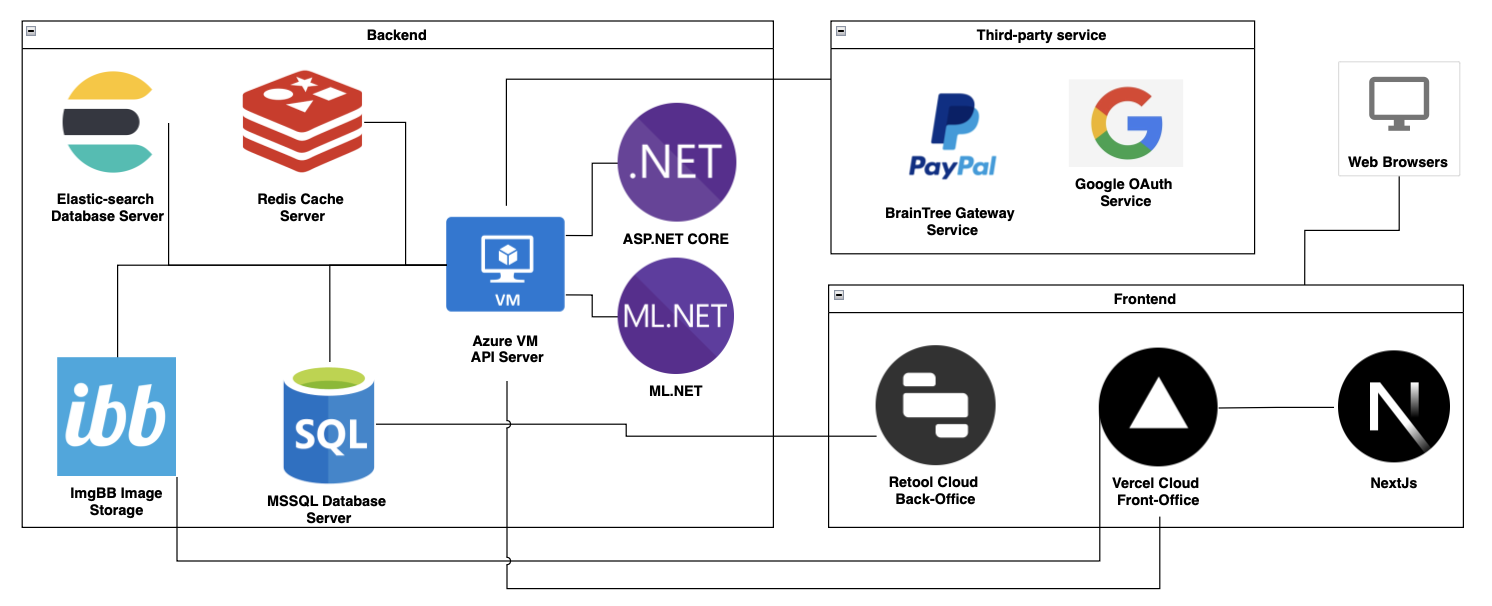
\includegraphics[width=1\textwidth]{Figures/Deployment/architect-report.png}
    \caption{Architecture Diagram}
    \label{fig:deployment-architecture}
\end{figure}
The Frontend component contains the back office and front office website of the system. This component is served to end users through web browsers.
\begin{itemize}
    \item \textit{Front office} handles user events and calls restful APIs from the API Server. It is implemented using Next.js and deployed on Vercel.
    \item \textit{Back office} is implemented using Retool. It interact directly to the MSSQL Database Server.
\end{itemize}

The backend of the system includes components as follows:
\begin{itemize}
    \item \textit{API Server} is the central part of the system, focusing on 
    handling all business logics and flows, serving API for the front office, 
    and interacting with other components of the system. It is implemented by ASP.NET Core and ML.NET and deployed by an Azure Virtual Machine.
    \item \textit{MSSQL Database Server} is the place where the database of the system is served. 
    This server interacts with the API Server and the back office.
    \item \textit{Imgbb Image Server} stores all the static images of the system. Images will 
    be uploaded directly from the front office to the Imgbb Image Server before storing the returned URLs in the SQL Database Server. This component will 
    be served by a free Imgbb cloud service.
    \item Furthermore, we will have two corresponding servers for caching data and optimizing 
    data search speed using a free \textit{Elastic-search cloud} and \textit{Azure Redis Cache Database}.
\end{itemize}

Finally, third-party services for authentication (Google OAuth Service) and payment (BrainTree Gateway Service) purposes are implemented by connecting to the API Server.

\section{UI/UX design}

In this section, we delve into the UI/UX design for our pet adoption website. Each page has been crafted to enhance user engagement and streamline the adoption process. Begins on the homepage, where users are welcomed with an intuitive interface that serves as the gateway to the platform. The login and register pages provide a seamless onboarding experience, ensuring a secure and personalized environment. The pet search page facilitates effortless exploration, allowing users to discover potential companions with ease. Detailed pet profiles showcase comprehensive information, fostering informed decision-making. The user profile page ensures a tailored experience, while the blog homepage and pages provide valuable insights and updates. To navigate this cohesive ecosystem, a diagram illustrates the interconnectedness of each page, illuminating the user's journey from entry to adoption. To enhance clarity, we've included a comprehensive diagram illustrating the intricate connections between these pages
\subsection{Front office}

\begin{figure}[H]
    \centering
    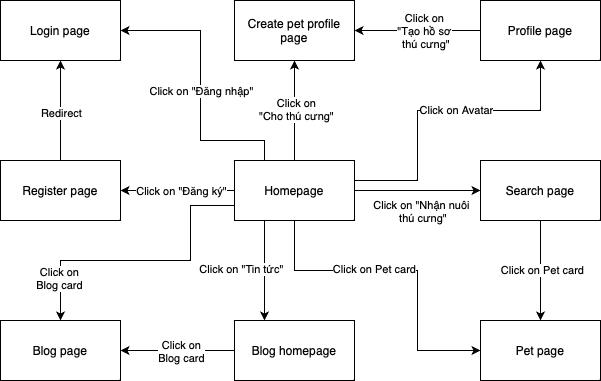
\includegraphics[width=0.8\textwidth]{Figures/wireframe_fo.png}
    \caption{Wireframe for Front office}
\end{figure}

\subsubsection{Homepage}

The homepage serves as the focal point of our pet adoption website, designed with a user-centric approach to ensure an intuitive and engaging experience. The navigation bar stands as a gateway to key functionalities, allowing users to seamlessly register, log in, explore pet profiles, create their pet profiles, access insightful blog content, and manage their user profile. The strategic placement of these navigation options facilitates effortless interaction. The hero section captures attention with visually appealing imagery and succinct messaging, encapsulating the essence of our mission. The "About Us" section provides a deeper understanding of our organization, building trust and connection with our audience. Additionally, the organization section offers insights into our partners and collaborators, fostering a sense of community.

\begin {figure}[H]
\centering
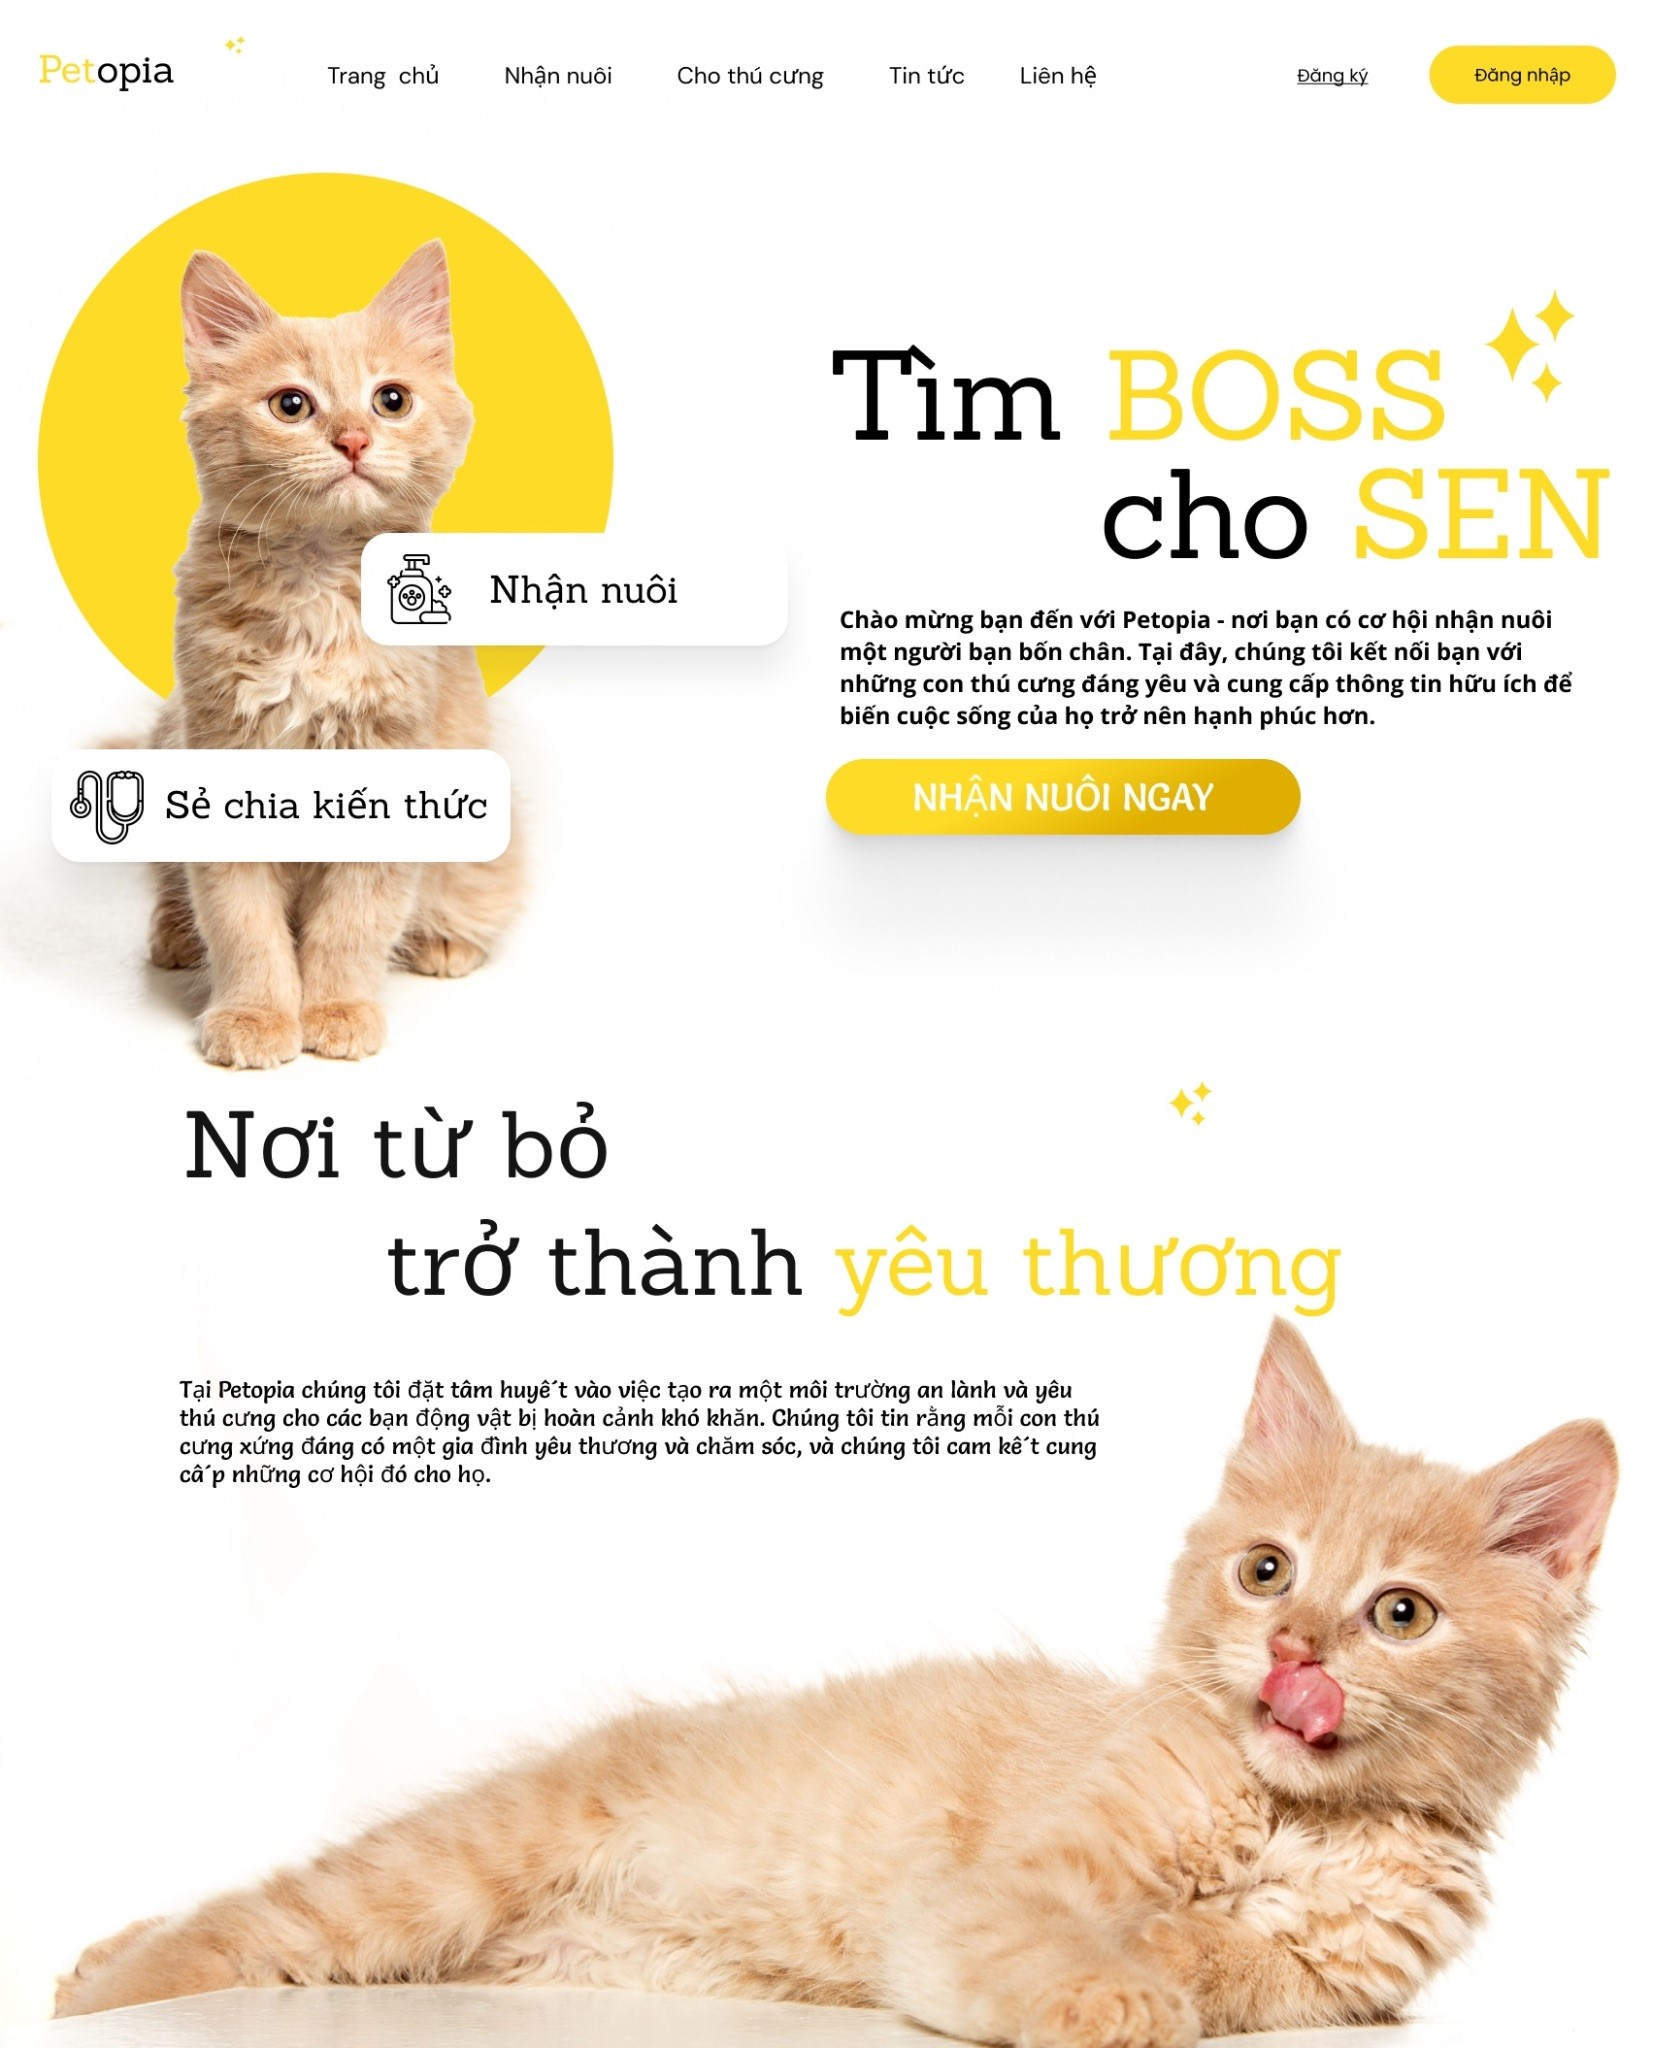
\includegraphics[width=0.8\textwidth]{Figures/UI/home_ui.jpg}
\caption{Homepage of Petopia}
\end{figure}

\subsubsection{Login}

Our homepage's login functionality is designed for simplicity and security, providing a seamless entry into the pet adoption experience. Users can access the login page with a click on the "Đăng nhập" button, where they input their Gmail and password. Error notifications guide users in case of issues, and a convenient register button directs new users to the registration page. For accessibility, users can also log in using their Google account, streamlining the process. A "Forgot Password" option is available for password resets, ensuring a hassle-free and secure experience that accommodates diverse user preferences.

\begin{figure}[H]
    \centering
    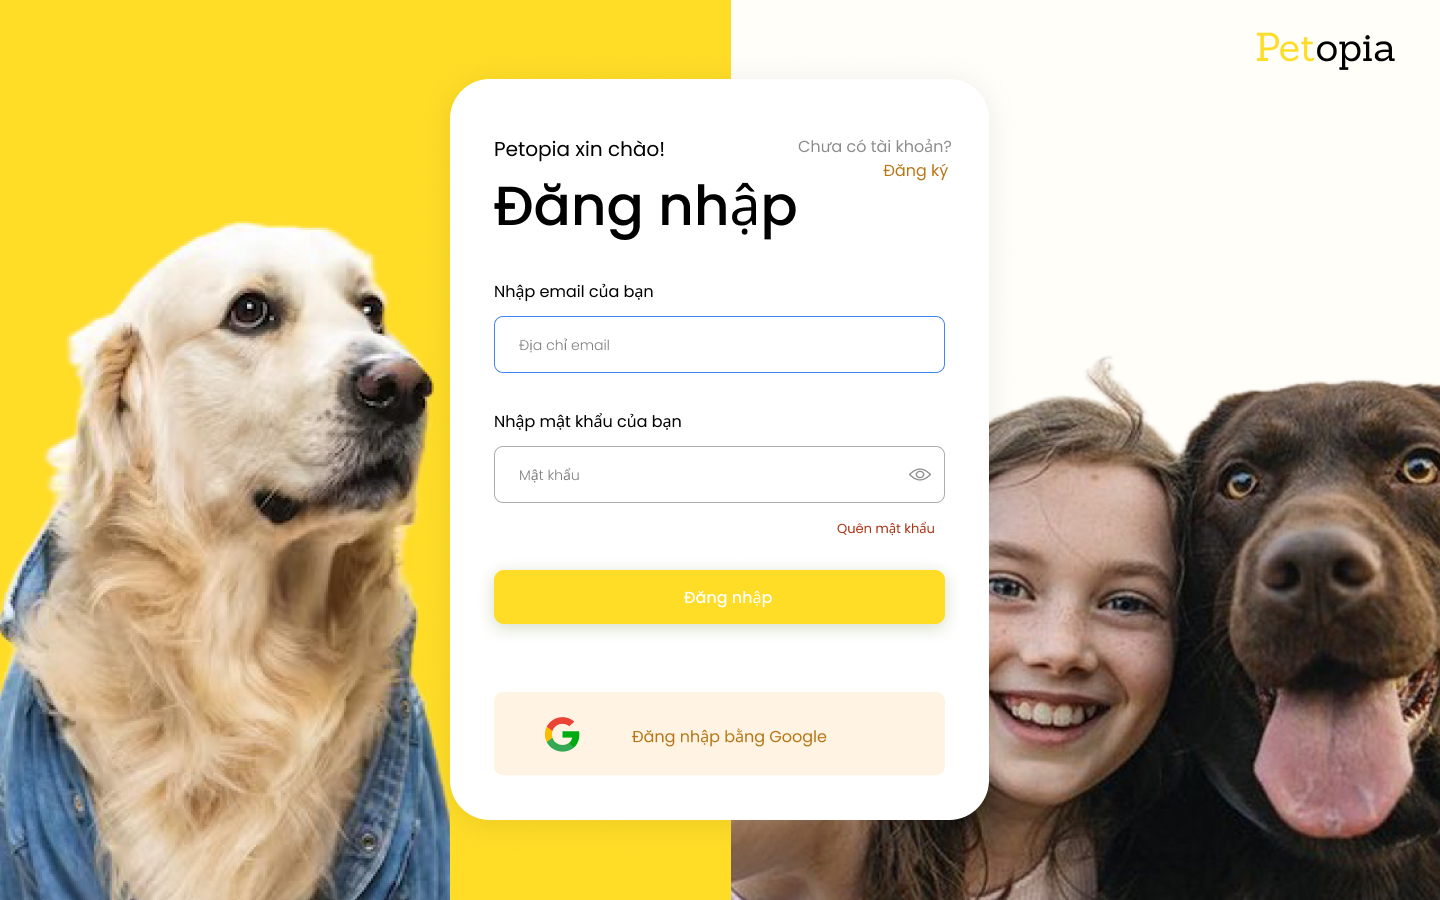
\includegraphics[width=0.8\textwidth]{Figures/UI/login_ui.png}
    \caption{Login form}
\end{figure}

\subsubsection{Register}

The registration process is straightforward, requiring users to input essential information such as first name, last name, Gmail, and password. After clicking "Register," the system verifies the form's completeness and prompts users to check their email for account verification. A verification link enhances security, ensuring authenticity. Clicking the link redirects users to the login page, confirming successful account creation. This two-step process prioritizes security and user-friendly guidance, fostering trust in our platform.

\begin{figure}[H]
    \centering
    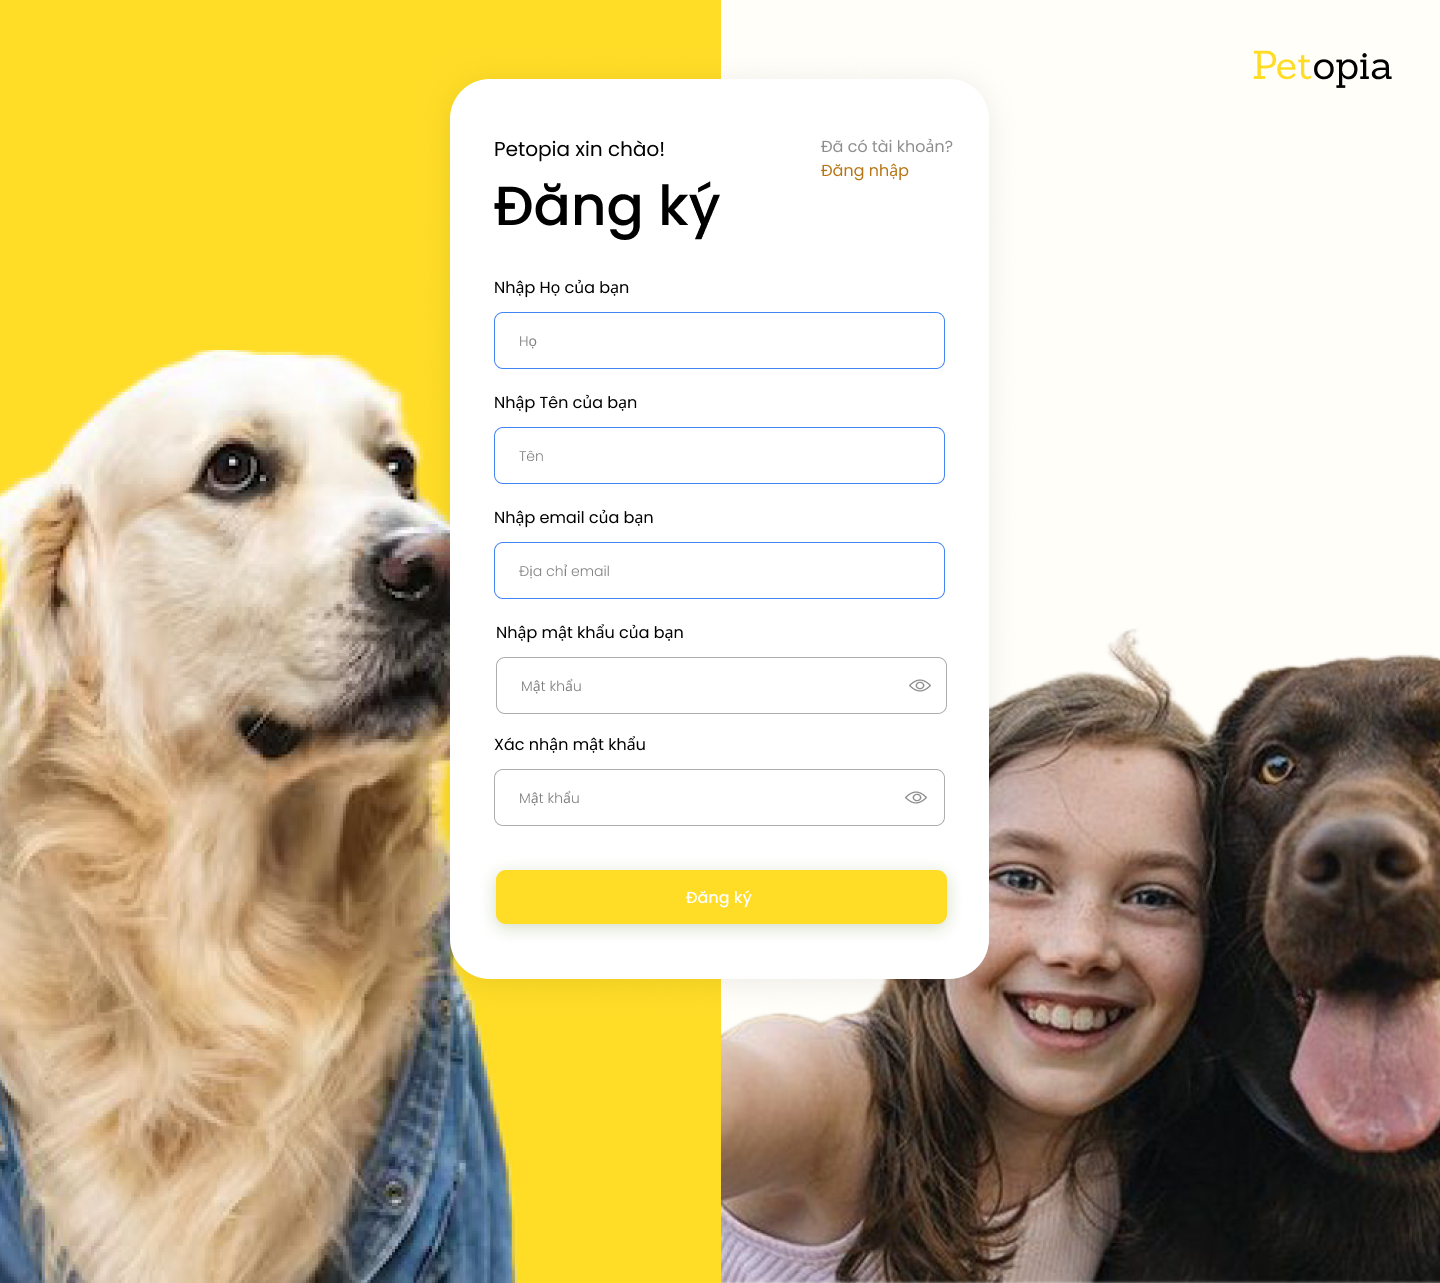
\includegraphics[width=0.5\textwidth]{Figures/UI/register_ui.png}
    \caption{Register form}
\end{figure}

\subsubsection{Search page}

The pet search page is designed for precision and ease. Users can tailor their search 
with checkboxes for sex, breed, color, size, and vaccination status. A sorting feature 
arranges results for flexibility. A prominent search bar, and supporting text and image
 queries, ensure a personalized and efficient experience. Robust filtering, sorting, and 
 versatile search methods aim to provide a user-friendly pet discovery journey on our platform.

\begin{figure}[H]
    \centering
    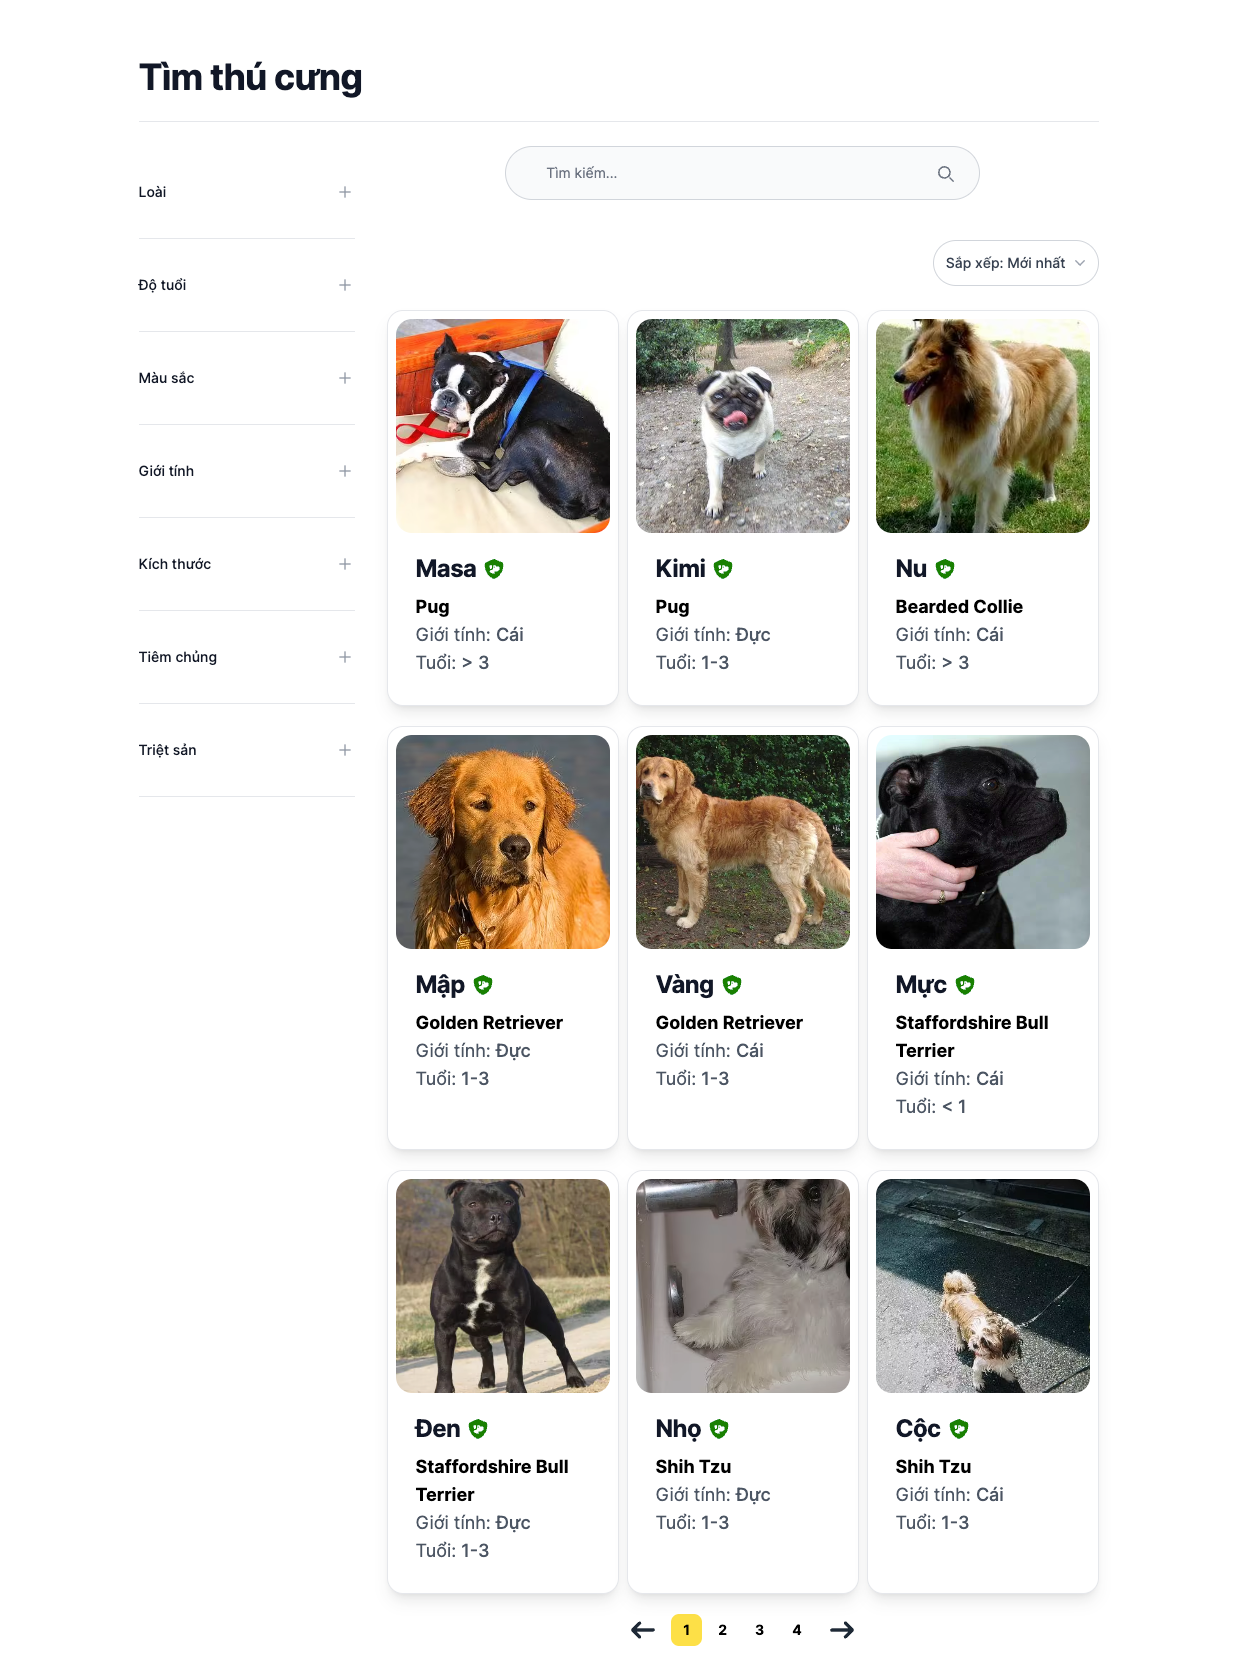
\includegraphics[width=0.8\textwidth]{Figures/UI/search_ui.png}
    \caption{Search page for searching desired pet}
\end{figure}


\subsubsection{Pet profile}

The pet page is a comprehensive showcase, providing detailed insights into each pet. Clicking on a pet card redirects users to the dedicated pet profile page, displaying key information such as name, breed, age, and vaccination status. Striking images and a personal description offer a deeper understanding of the pet's personality. A prominent "Adopt" button facilitates the adoption process, dynamically revealing an efficient adoption form upon click. This ensures transparent communication between potential adopters and pet owners.

\begin{figure}[H]
    \centering
    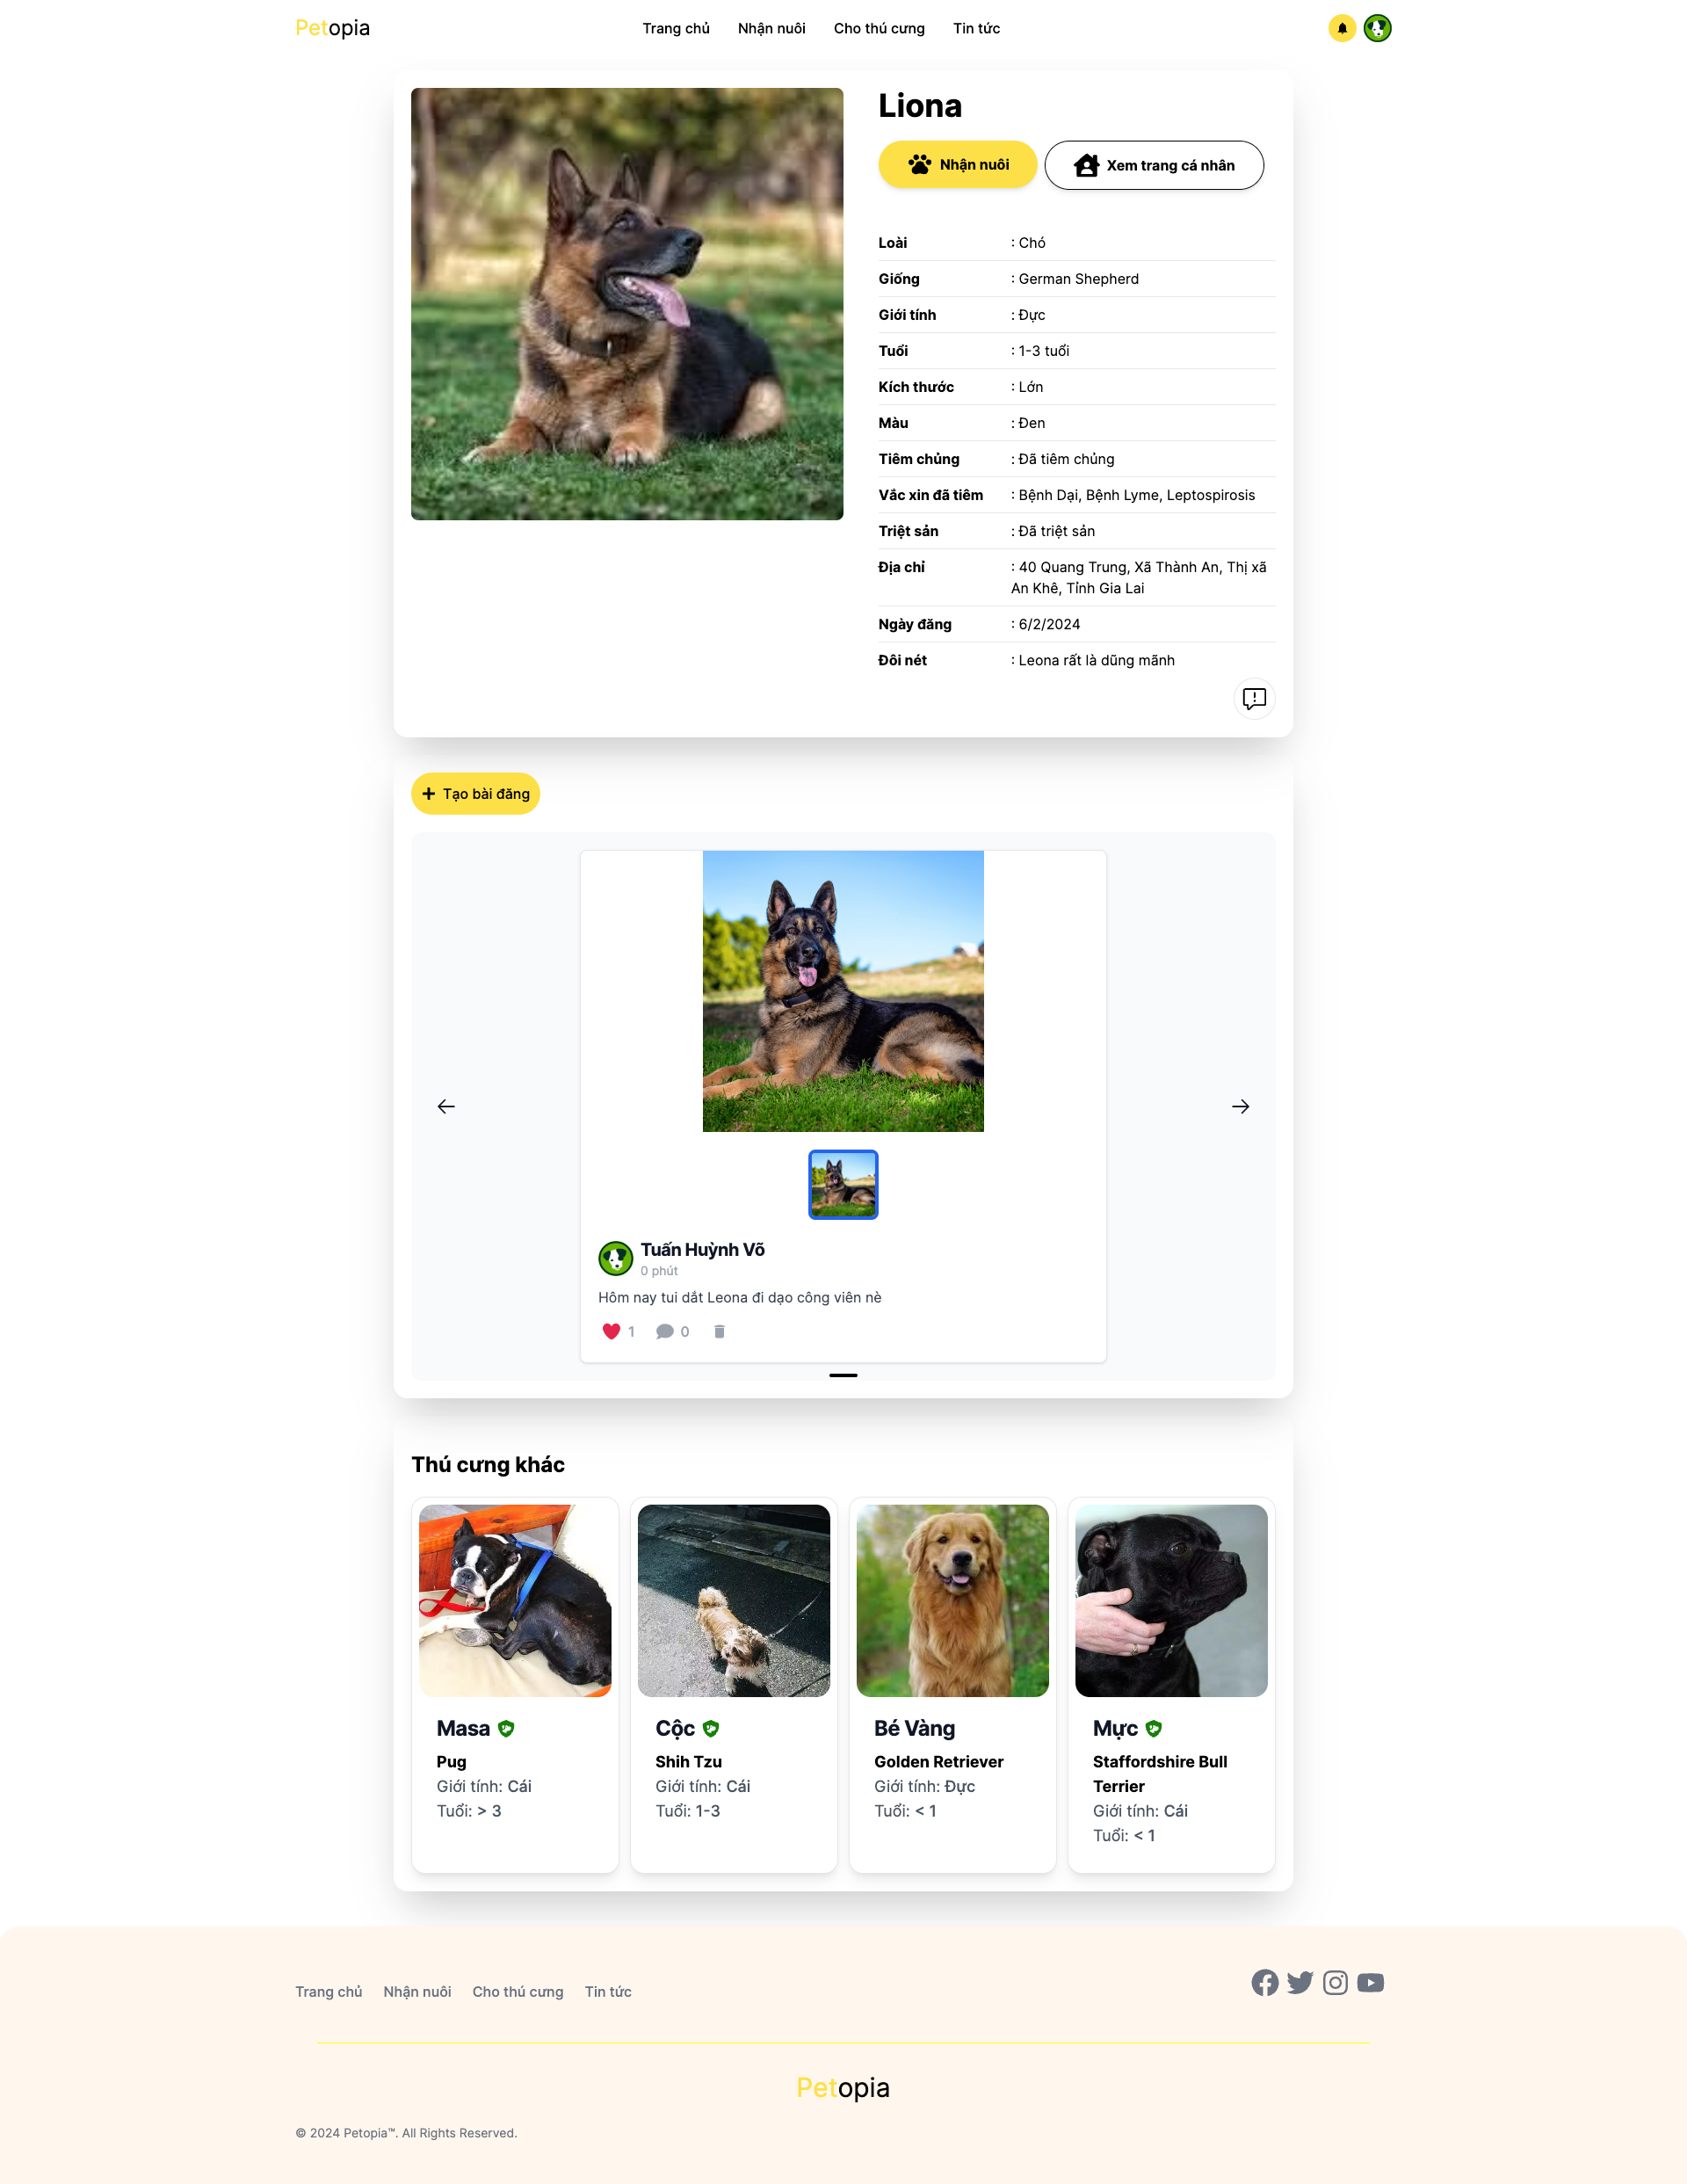
\includegraphics[width=0.6\textwidth]{Figures/UI/pet_detail_ui.png}
    \caption{Pet profile page}
\end{figure}

\subsubsection{Create pet profile}

\begin{figure}[H]
    \centering
    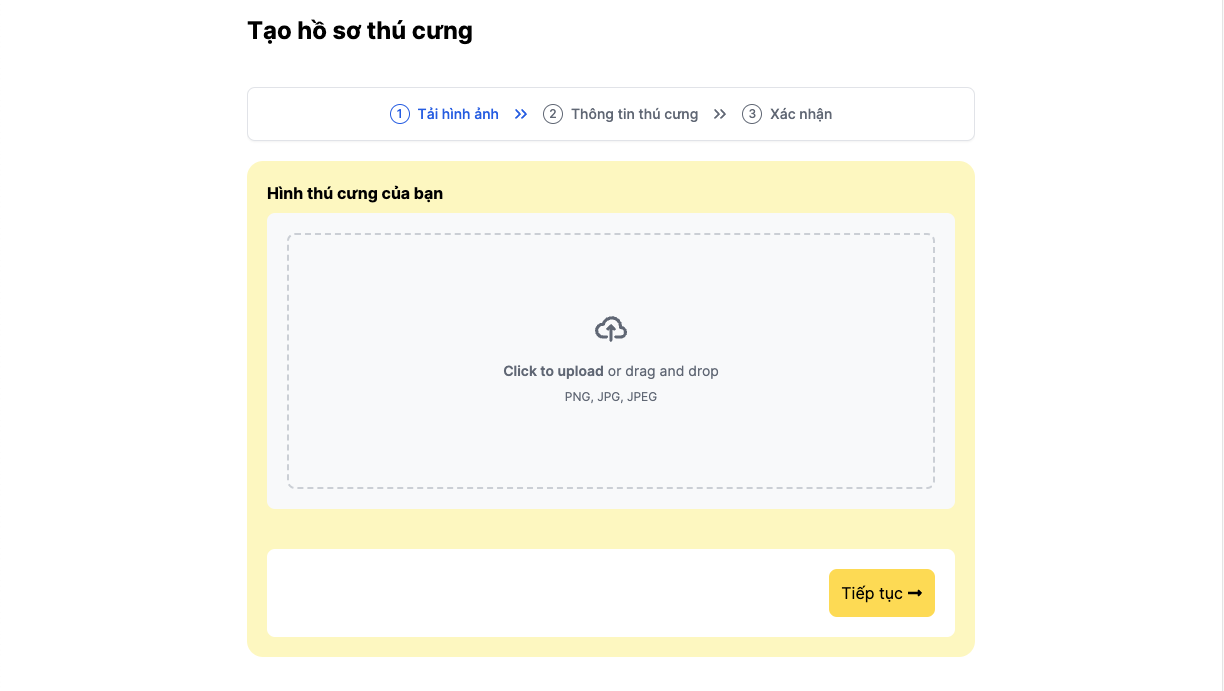
\includegraphics[width=0.6\textwidth]{Figures/UI/image_upload_ui.png}
    \caption{Image upload form}
\end{figure}

\begin{figure}[H]
    \centering
    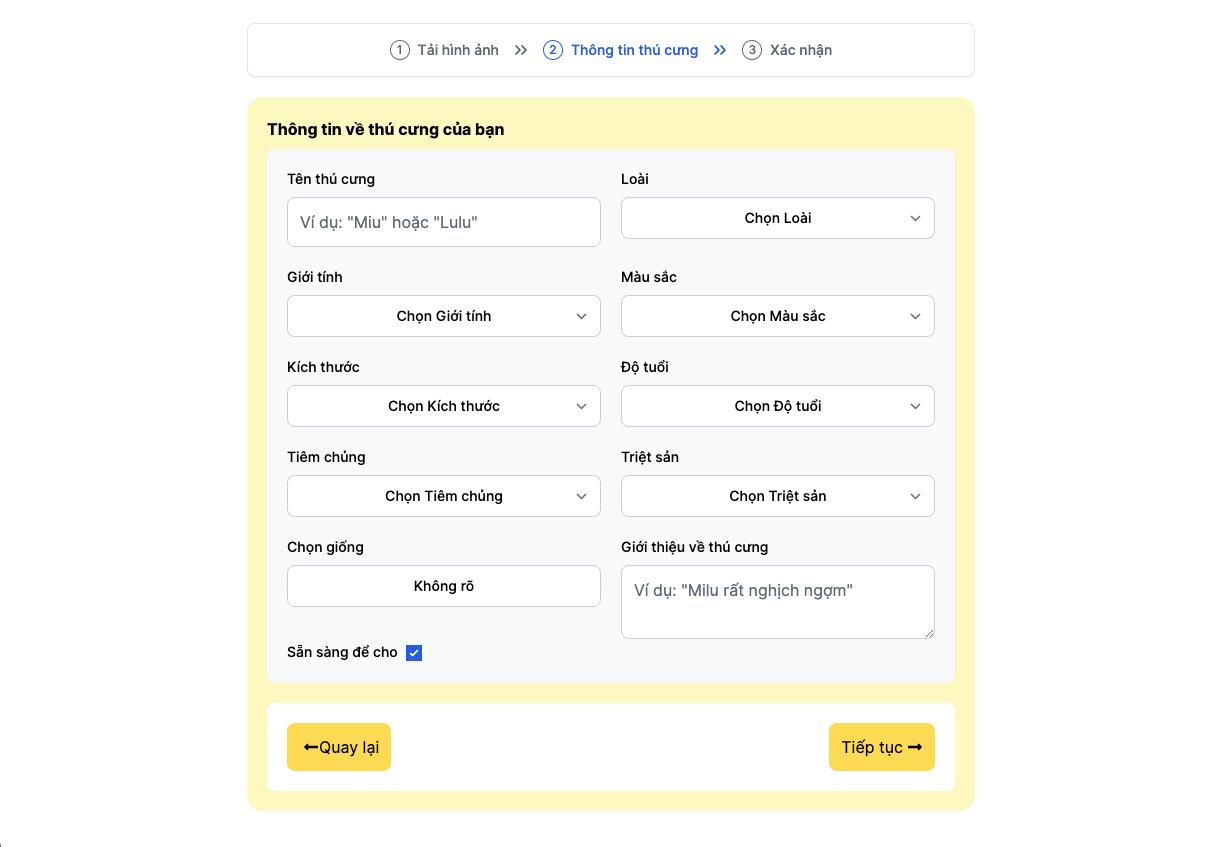
\includegraphics[width=0.6\textwidth]{Figures/UI/pet_input_ui.png}
    \caption{Form for taking user's pet detail}
\end{figure}

\begin {figure}[H]
\centering
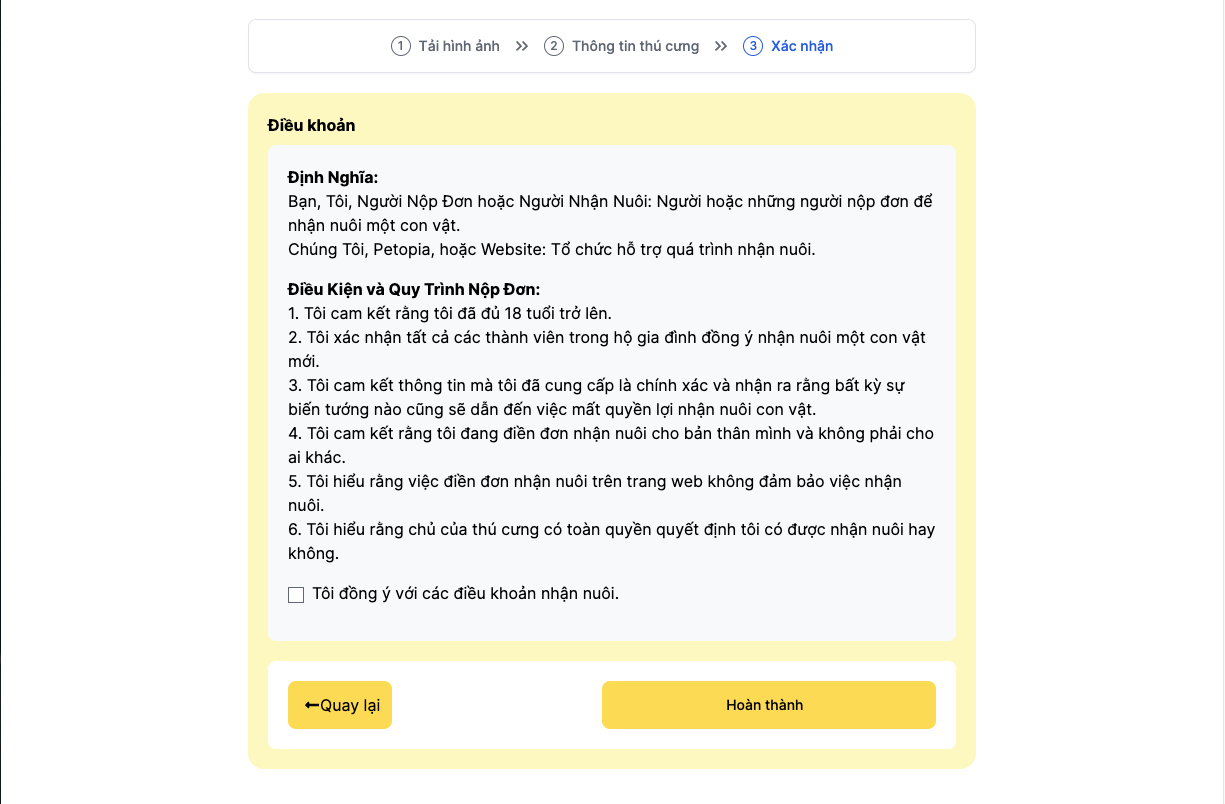
\includegraphics[width=0.6\textwidth]{Figures/UI/term_ui.png}
\caption{Pet profile page}
\end{figure}

Creating a pet profile on our platform is user-friendly and efficient. Users begin by uploading a pet image (Figure 3.8), which our AI processes to autofill the breed. Clicking "Continue" leads to a detailed pet form (Figure 3.9) for additional information. Users then review the Terms and Services (Figure 3.10) before clicking "Finish" to complete the profile. This structured process, with AI assistance in the initial steps, ensures accuracy and a seamless user experience.

\subsubsection{User profile}

\begin{figure}[H]
    \centering
    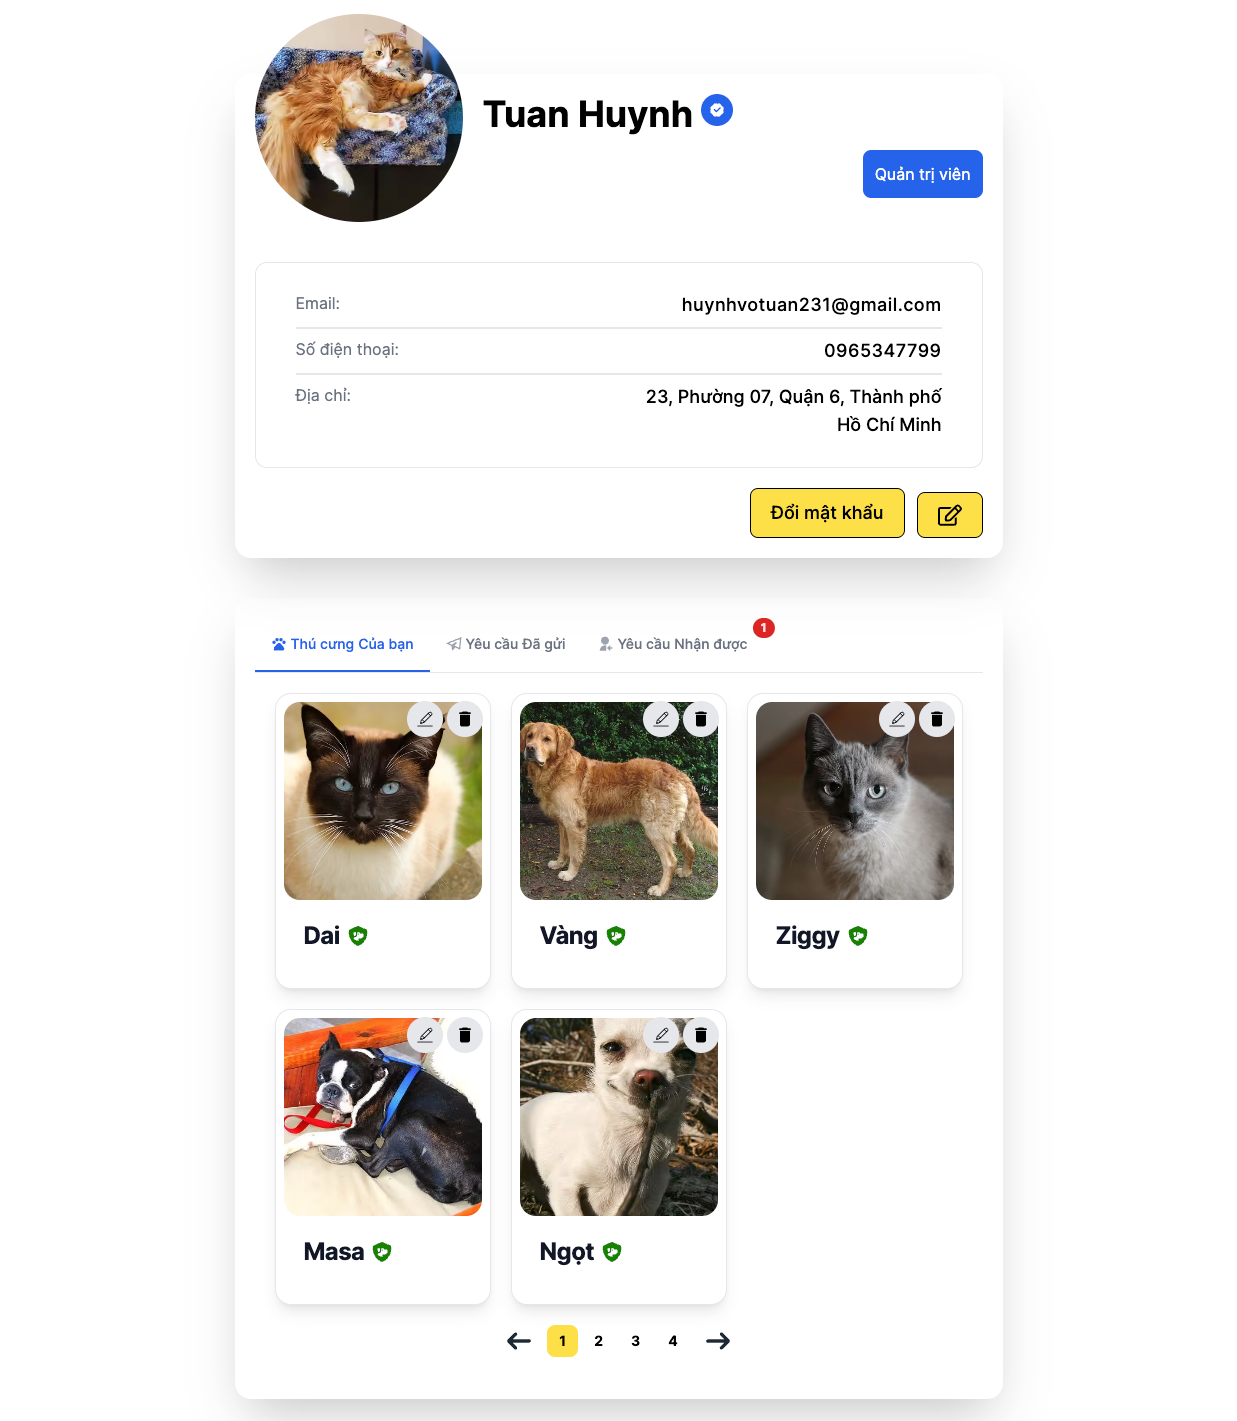
\includegraphics[width=0.7\textwidth]{Figures/UI/user_profile_ui.png}
    \caption{User profile page}
\end{figure}
The user profile page serves as a centralized hub for managing and personalizing 
information, offering a seamless and enjoyable experience. At the top, users will 
find their avatar, name, address, Gmail, and phone number, all of which can be easily 
edited to keep details up-to-date. User can also change their password or update information in this page. The page also features pet profiles, allowing 
users to manage information about their pets effortlessly. Additionally, a management
 table includes tabs for Sent and Incoming messages, notifying users about adoption
  requests and the status of their adoption forms. This intuitive design ensures 
  users can efficiently handle personal information and engage with our platform's
   pet adoption features.

\subsubsection{Organization profile}
\begin{figure}[H]
    \centering
    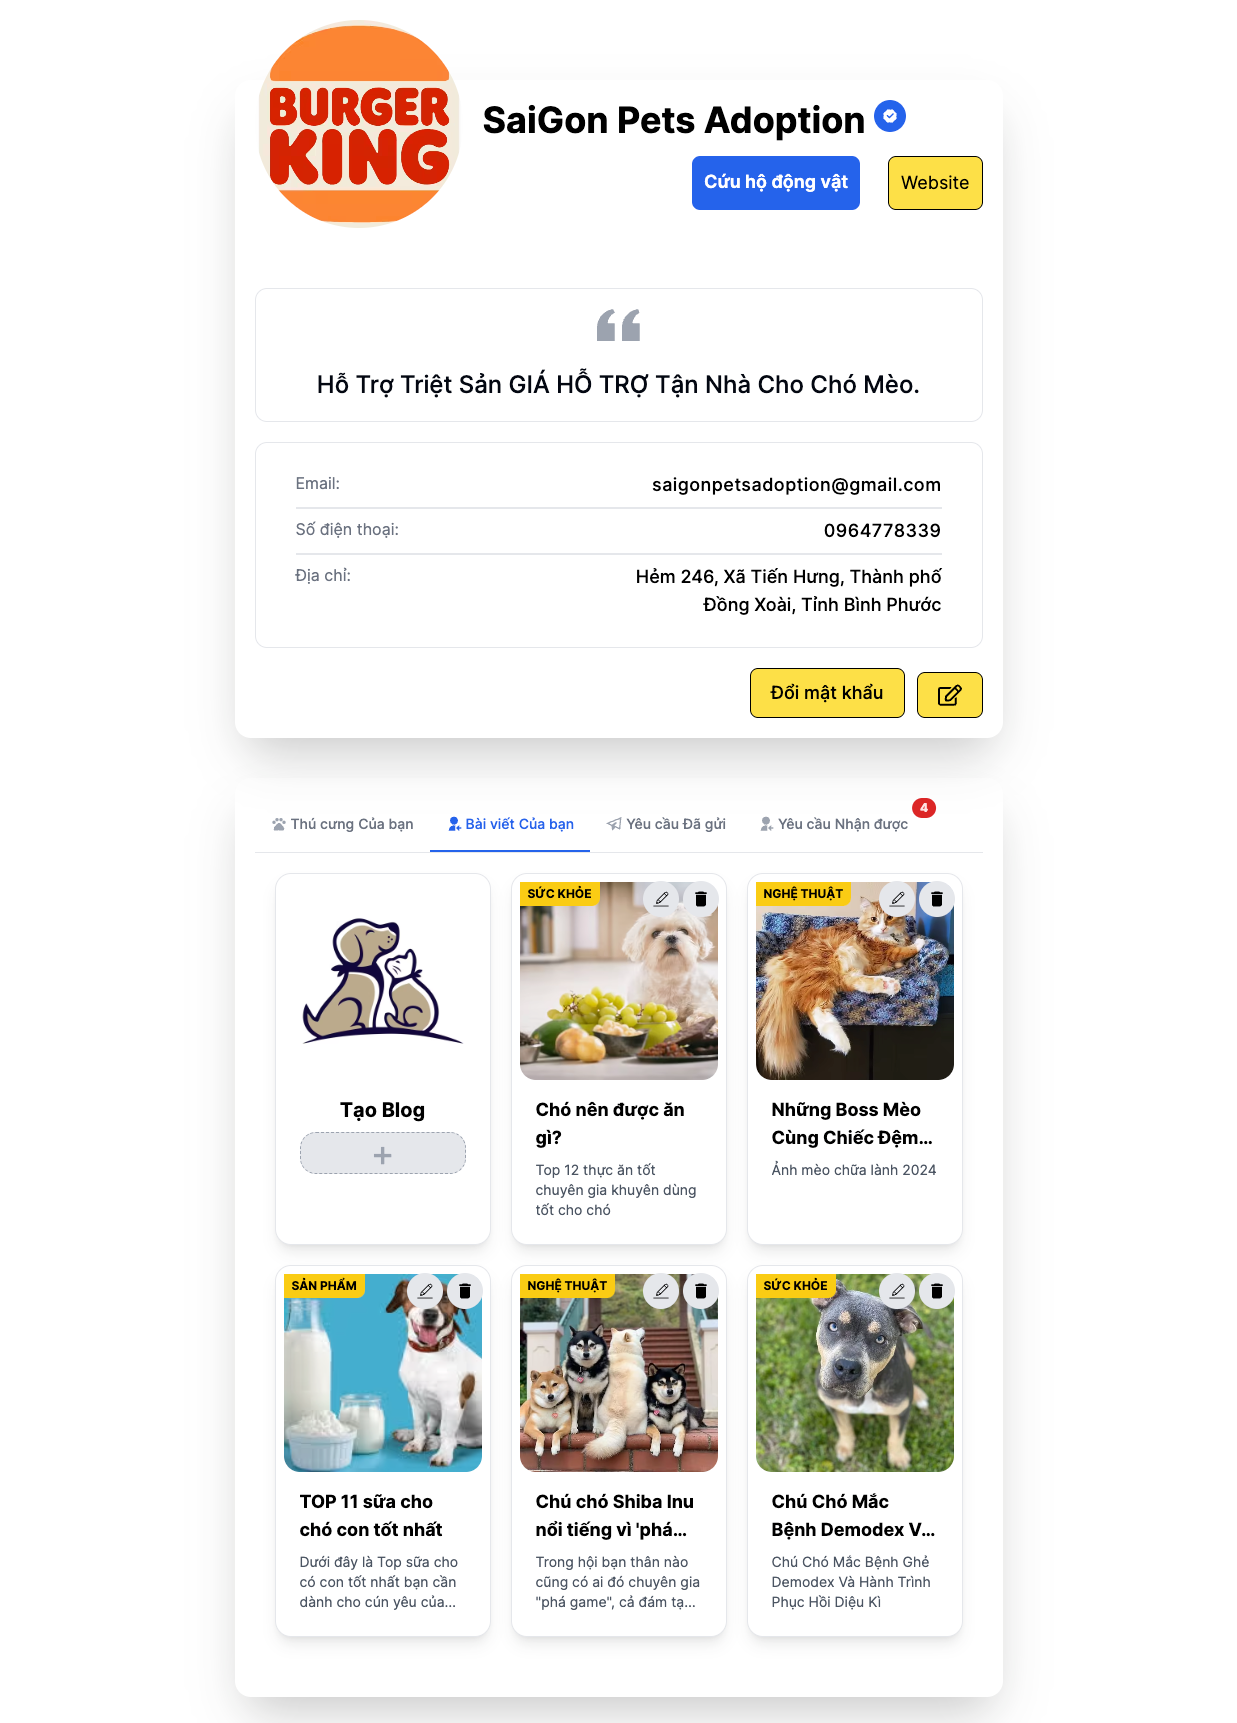
\includegraphics[width=0.7\textwidth]{Figures/UI/org_profile_ui.png}
    \caption{Organization profile page}
\end{figure}

The organization profile mirrors the user profile but includes a verification badge to confirm the account's authenticity. Beneath the organization name, a badge indicates the type of organization. This page also offers functions for changing passwords and updating information. In addition to basic details, the page includes the organization's slogan and web link. The management table features an extra blog tab, allowing users to create, update, or delete blog posts.

\subsubsection{Blog homepage}
\begin{figure}[H]
    \centering
    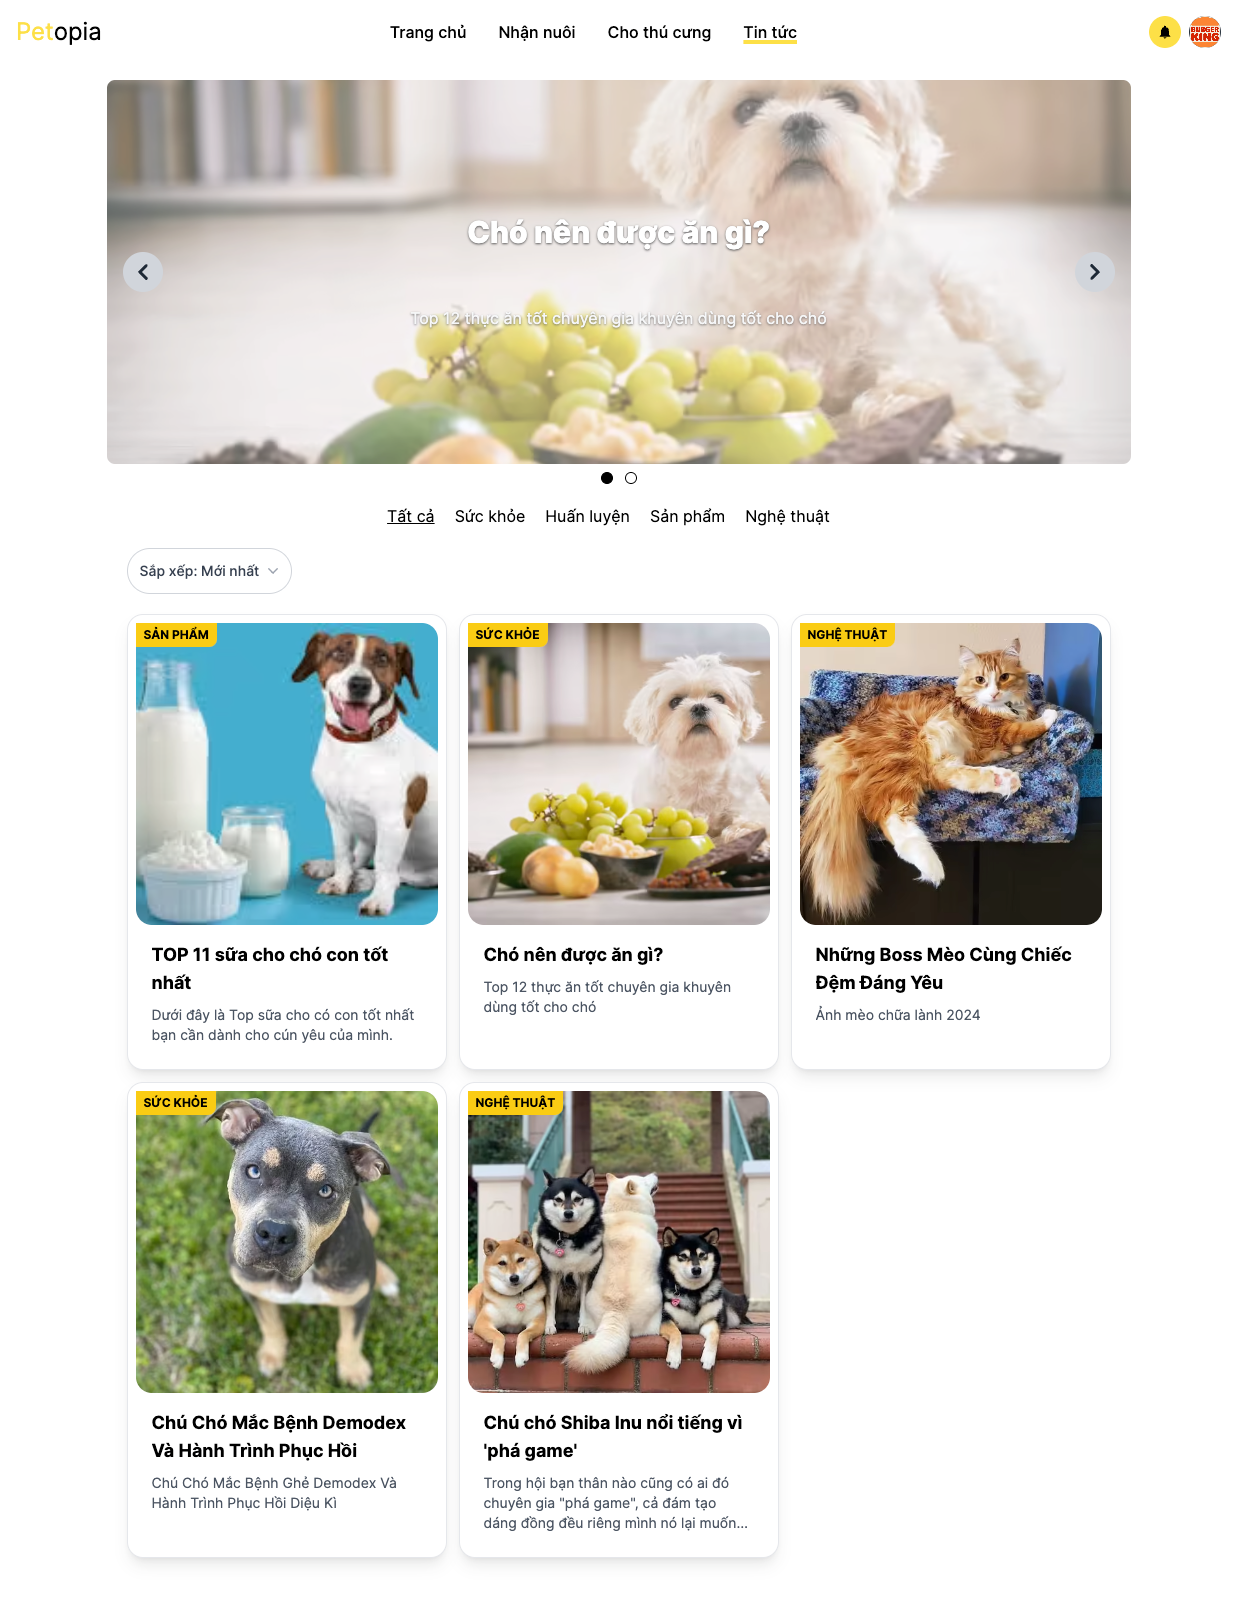
\includegraphics[width=0.8\textwidth]{Figures/UI/blog_ui.png}
    \caption{Blog homepage}
\end{figure}

The blog homepage offers a curated space with various categories for users to explore diverse content.
 Clicking a category dynamically displays relevant blogs, ensuring a targeted reading experience. 
 Selecting a specific blog seamlessly redirects users to the dedicated blog page for detailed 
 exploration. Integrated ads support the platform without disrupting the user experience, 
 contributing to the sustainability of our blog platform.

\subsubsection{Blog page}

\begin{figure}[H]
    \centering
    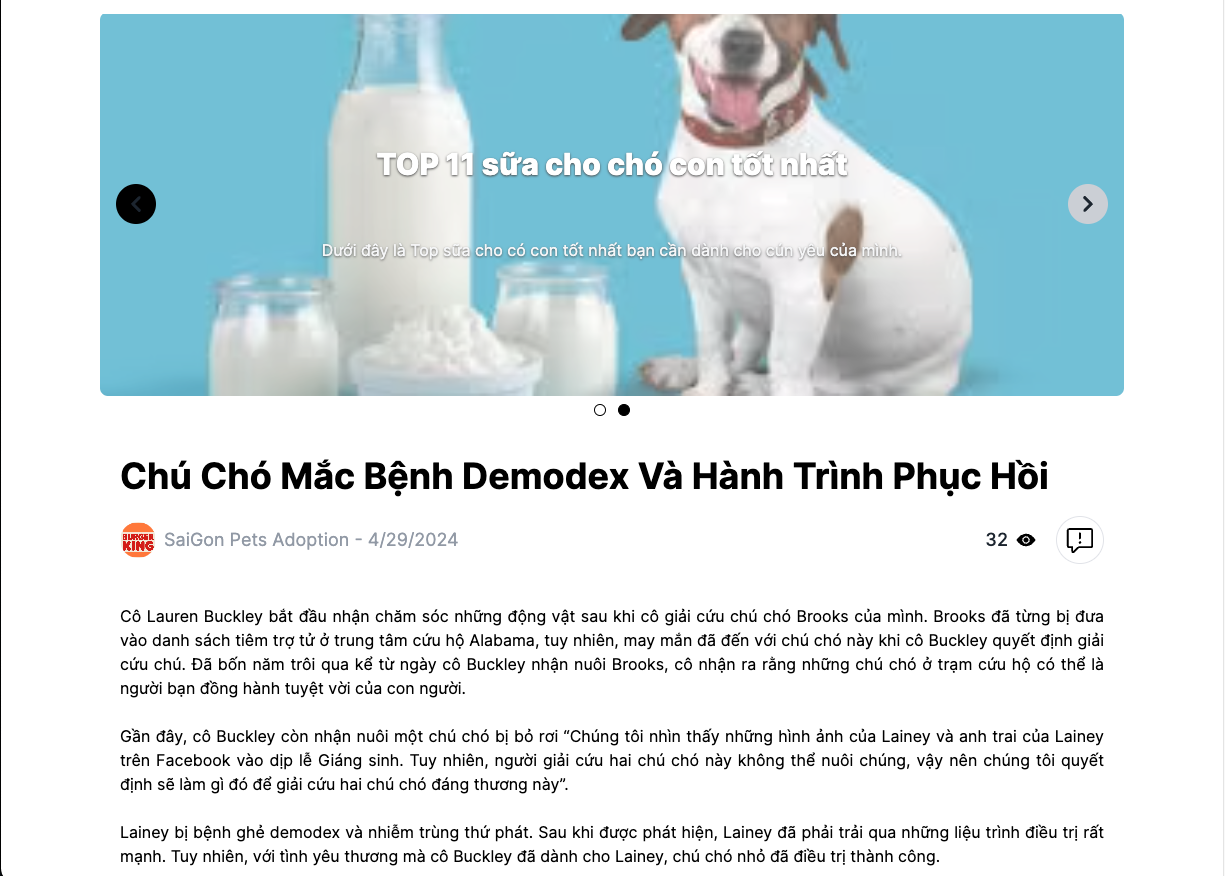
\includegraphics[width=0.8\textwidth]{Figures/UI/blog_page_ui.png}
    \caption{Blog page}
\end{figure}

The blog page ensures a rich and interactive reading experience, allowing users to delve into 
detailed blog posts. Metrics like view count indicate popularity. A relevant section suggests 
related blogs, encouraging users to explore aligned topics for an enhanced and curated experience.

\subsubsection{Payment page}
\begin{figure}[H]
    \centering
    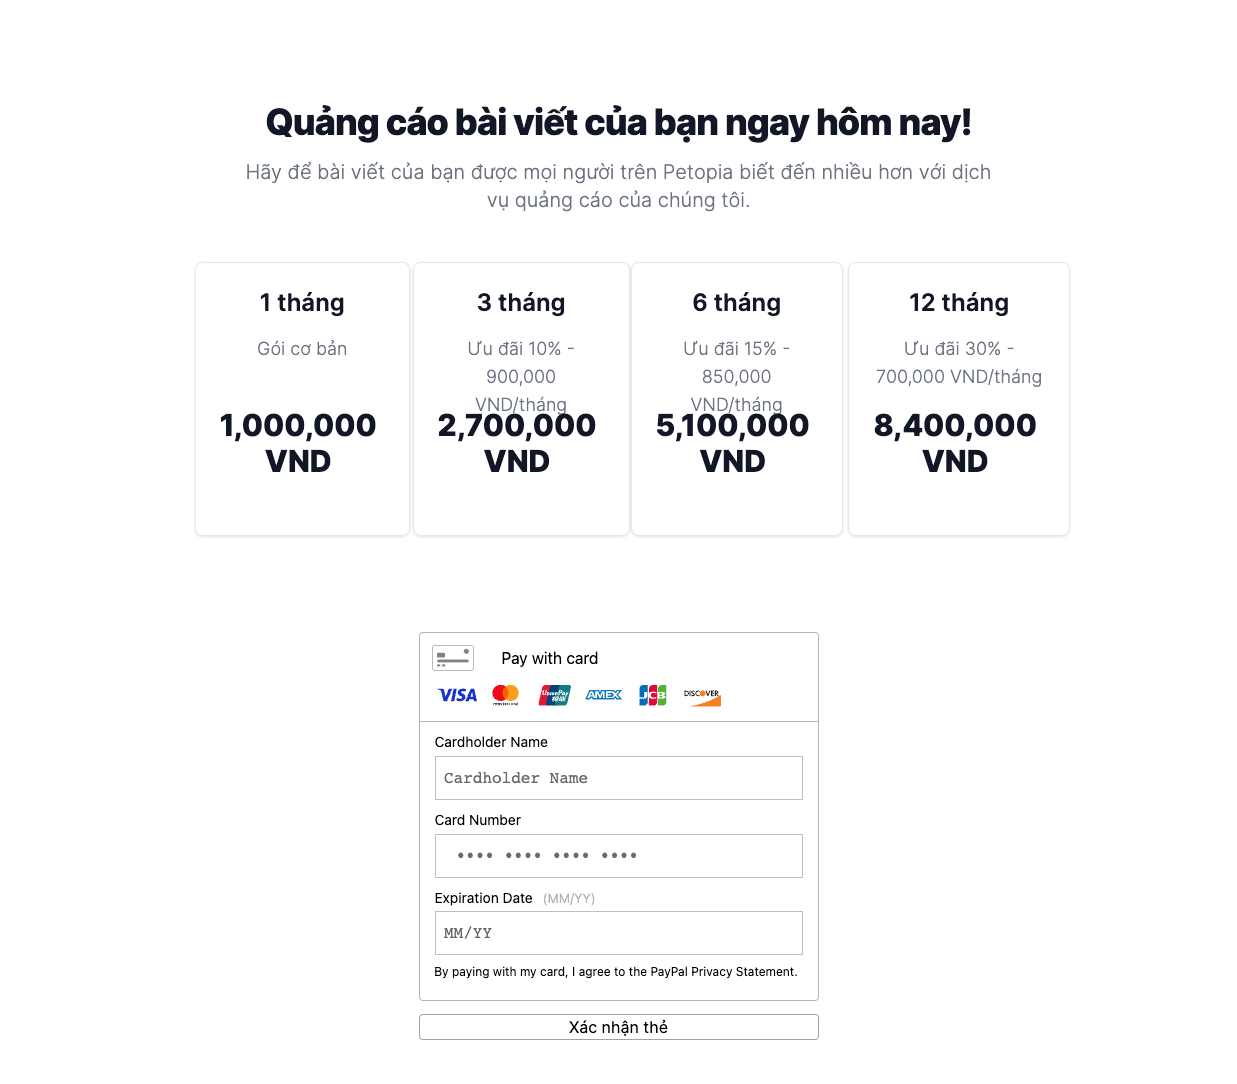
\includegraphics[width=0.8\textwidth]{Figures/UI/payment_ui.png}
    \caption{Payment page}
\end{figure}
On the payment page, users have the option to advertise their blog by selecting from one of four subscription plans: 1 month, 3 months, 6 months, or 12 months. Each plan offers varying levels of exposure and cost, allowing users to choose the duration that best fits their needs and budget. Once a plan is selected, users can proceed by entering their card information in the provided fields. The system ensures secure processing of the payment, after which the advertising plan will be activated. This streamlined process makes it easy for users to promote their blogs effectively.

\newpage
\subsection{Back office}

\subsubsection{Dashboard}

\begin{figure}[H]
    \centering
    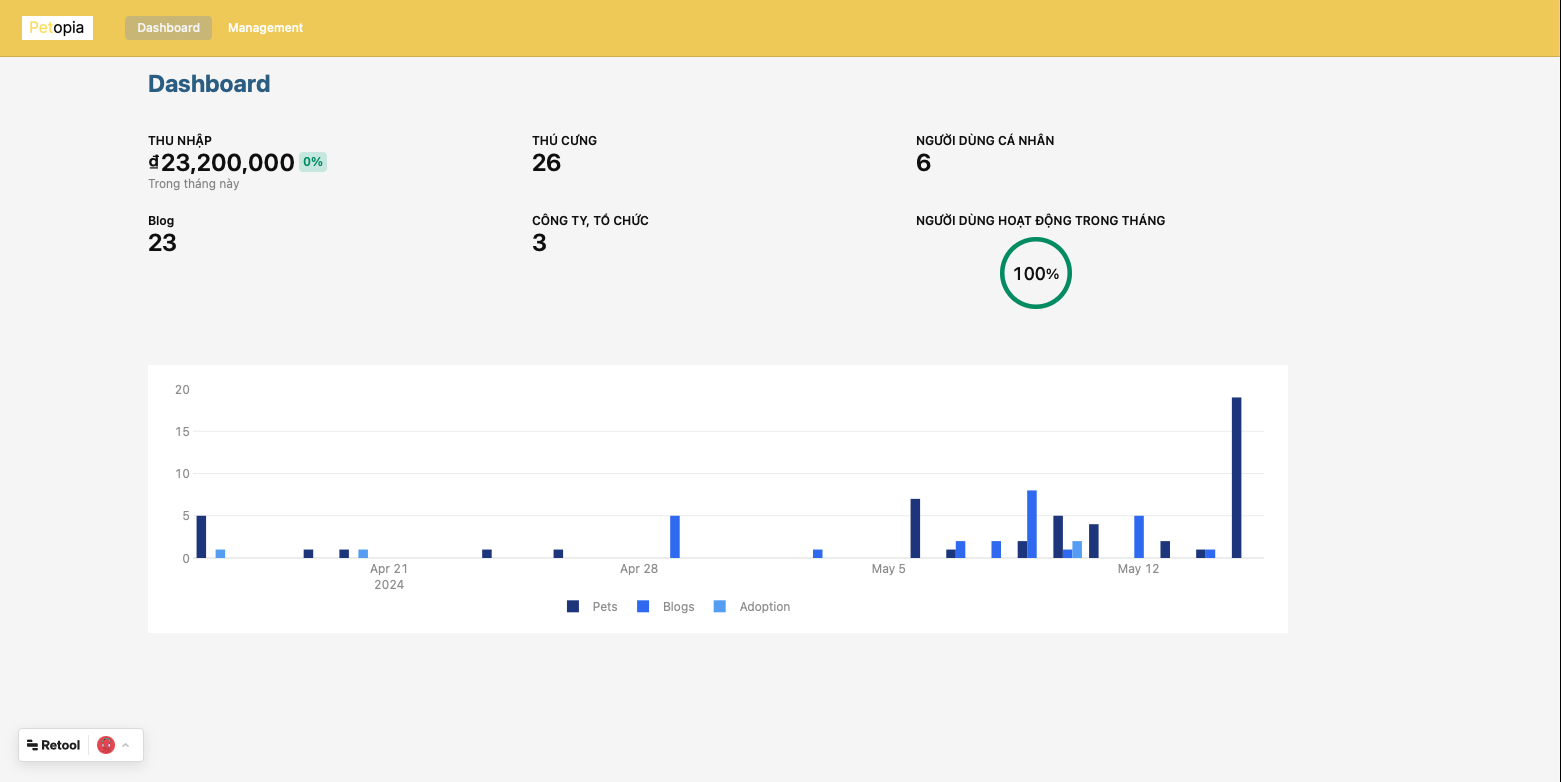
\includegraphics[width=0.7\textwidth]{Figures/UI/dashboard_bo_ui.png}
    \caption{Dashboard to show reports and statistics}
\end{figure}

The dashboard page provides administrators with comprehensive insights into the Petopia website. It displays key metrics such as the number of visitors, pets, blogs, and users. To enhance visualization, graphical representations accompany these statistics, offering a clear and dynamic overview of the platform's performance. This feature allows administrators to efficiently monitor and analyze the website's vital statistics at a glance.

\subsubsection{Control page}

The control page empowers administrators to manage specific data types, including users, blogs, and pets. Administrators can access records, apply filters for efficient navigation, edit fields, enable or disable records, and delete them as needed. This functionality provides administrators with a versatile and centralized tool for comprehensive control and customization of various data records on the platform.

\begin {figure}[H]
\centering
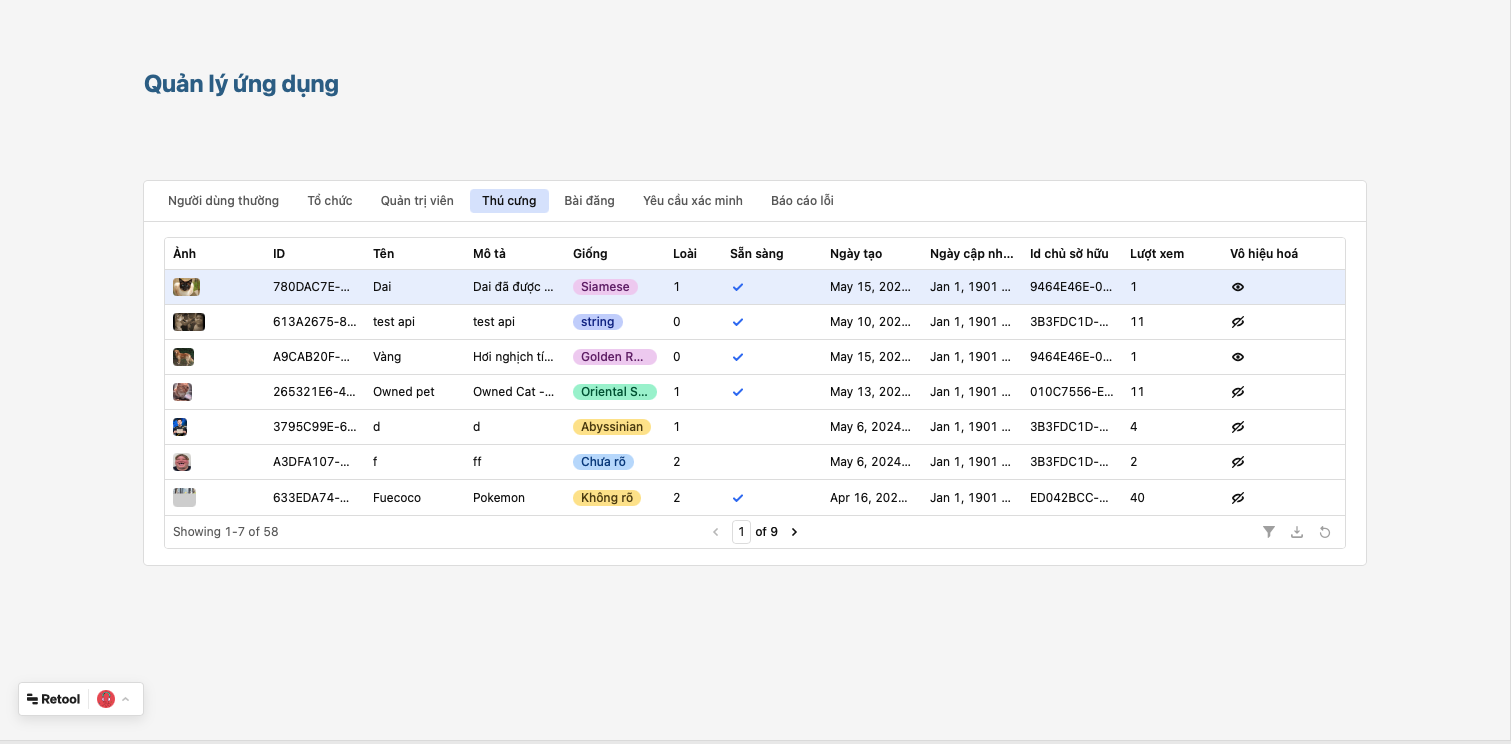
\includegraphics[width=0.7\textwidth]{Figures/UI/control_bo_ui.png}
\caption{Control page for managing data records}
\end{figure}

\newpage
\section{Database design}

\subsection{Conceptual design}

The conceptual design phase of the project is a pivotal stage in the development lifecycle, focused on establishing a comprehensive understanding of the system's structure and relationships.
\\
In \textit{Figure 3.18}, all entities and relationships are presented. Note that all attributes are excluded to enhance visualization and maintain a clear focus on the primary components shaping the system. These attributes will be shown in the physical design section.

\begin{figure}[H]
    \centering
    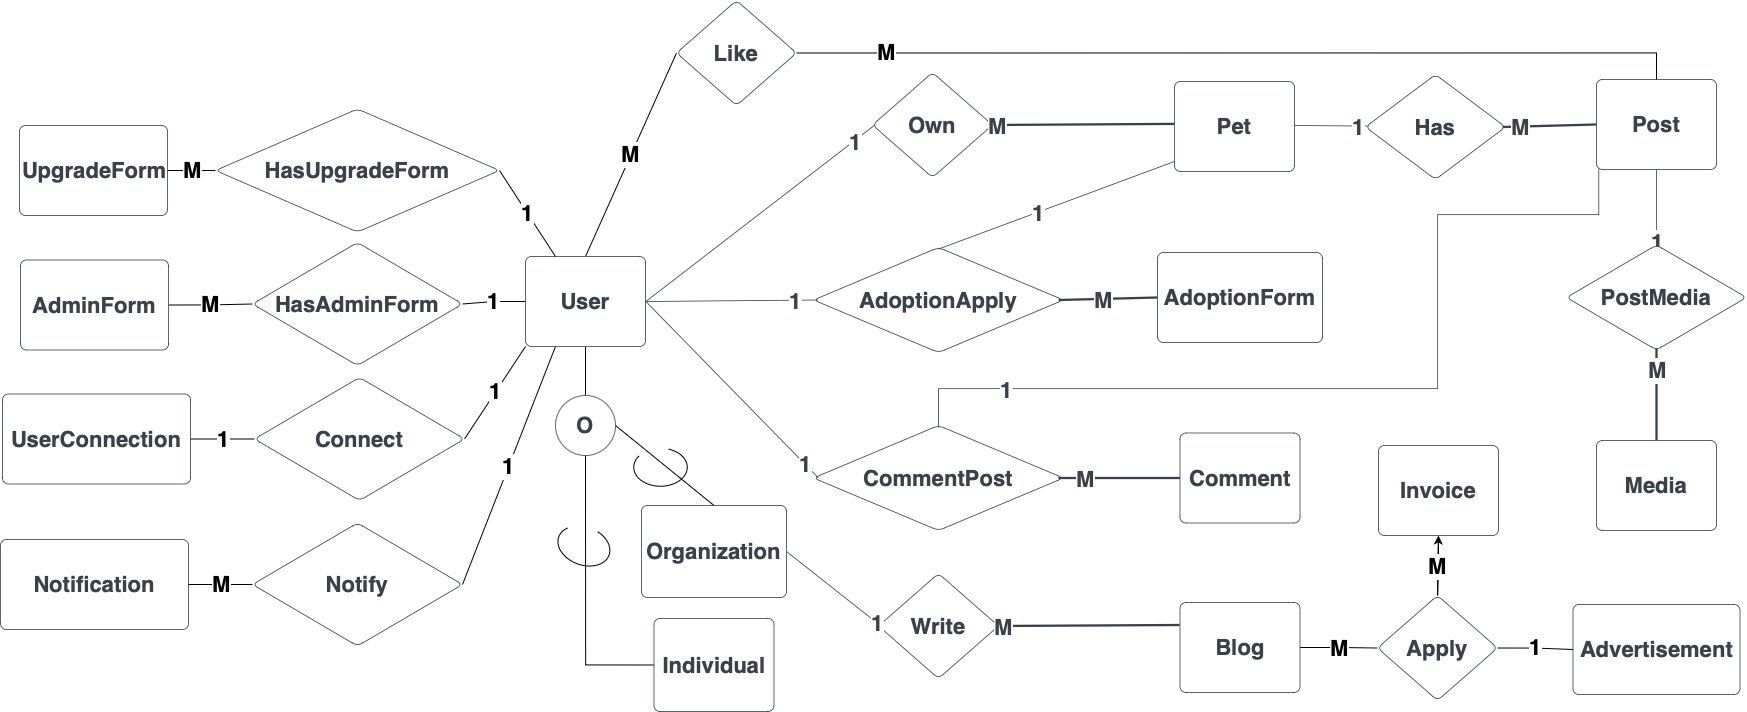
\includegraphics[angle=-90,width=0.4\textwidth]{Figures/DatabaseDesign/Entities-ERD.png}
    \caption{Entity-Relationship diagram}
\end{figure}
\clearpage

\subsection{Relational Design}

In the relational design phase, we use the relational mapping approach
to translate the abstract concepts from the Entity-Relationship Diagram
(ERD) into a concrete relational schema. Through the mapping process,
each entity, along with its attributes and relationships, is
systematically transformed into tables with defined fields and
corresponding constraints in \emph{Figure 3.19}.

\begin {figure}[H]
\centering
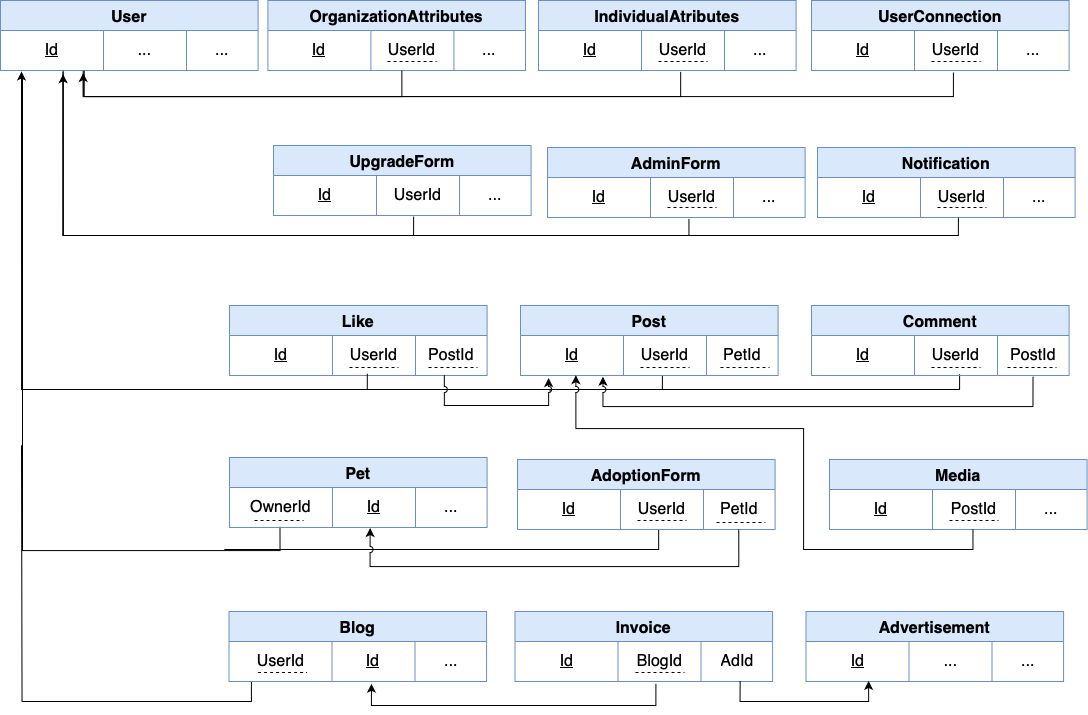
\includegraphics[width=0.9\textwidth]{Figures/DatabaseDesign/Entities-Mapping.png}
\caption{Relational schema}
\end{figure}

\emph{Figure 3.19}, the attributes are not presented fully to ensure a clear visualization of the diagram. In the relational mapping process, we implement a simplified technique for the 3-way relationship where the mandatory entity will take the primary key of the two optional entities as its foreign key, avoiding creating another table causes the schema to become unnecessarily complicated.

\subsection{Physical Design}

In this phase, the conceptual transforms into the tangible, as we build the actual blueprint that mirrors the intricacies of the adoption process in real life. The Relational Schema serves as our guidepost, detailing the tables, and relationships that will form the foundation of the physical database. \textit{Figure 3.20 and 3.21} below translates abstract entities and relationships into concrete data types and optimizes storage structures.

\begin {figure}[H]
\centering
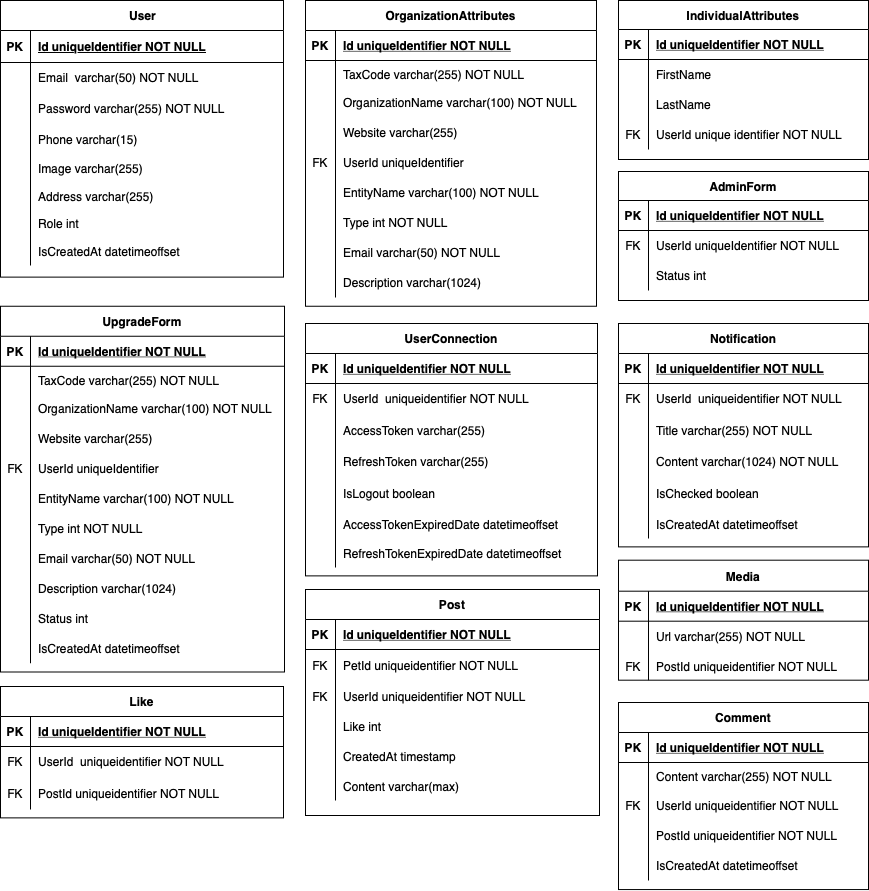
\includegraphics[width=0.8\textwidth]{Figures/DatabaseDesign/Entities-Physical_1.png}
\caption{Physical design}
\end{figure}

\begin {figure}[H]
\centering
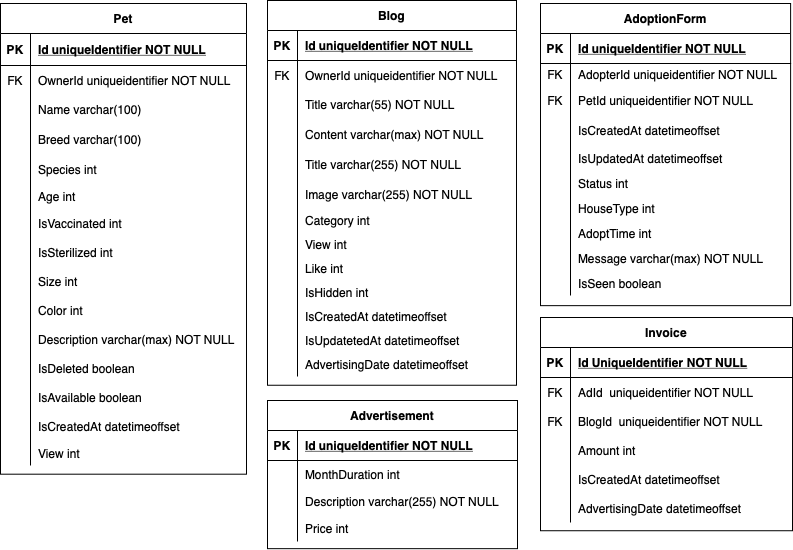
\includegraphics[width=0.8\textwidth]{Figures/DatabaseDesign/Entities-Physical_2.png}
\caption{Physical design (cont)}
\end{figure}





\chapter{DEVELOPMENT TECHNOLOGIES}

\section{Front-end}


In this section, we will dive into Next.js and Tailwind CSS. Next.js is
a React framework with features like server-side rendering, while
Tailwind CSS is a utility-first framework for streamlined styling
through pre-designed classes. These tools play a key role in creating
efficient and scalable front-end experiences.


\subsection{NextJS}

Next.js, a robust React framework, tackles challenges in traditional
client-side rendering. It utilizes server-side rendering and static site
generation to address accessibility, security, page loading times, and
Search engine optimization (SEO) concerns. Popular in the React
ecosystem, Next.js optimizes the user experience by pre-rendering pages
on the server. Advantages include enhanced performance with server-side
rendering, seamless React integration for dynamic interfaces, static
site generation for optimal website performance, intuitive file
system-based routing, automatic code splitting, flexible styling
approaches, and compatibility with TypeScript for improved code quality.


\subsection{Tailwind CSS}

Tailwind CSS, a utility-first framework, transforms web styling by
providing an extensive set of classes directly within HTML. This
accelerates development by offering granular control over layout, color,
spacing, and more. Unlike traditional CSS, Tailwind\textquotesingle s
unique approach eliminates the need for external files, enabling
seamless customization and efficient creation of visually appealing and
responsive interfaces. Its utility-first approach minimizes unused CSS,
optimizing performance, and its low learning curve, active community,
and integration flexibility make it an efficient choice for building
well-styled and maintainable web applications.


\section{Back-end}

\subsection{ASP.NET core platform}

ASP.NET Core, an open-source framework, excels in developing modern,
cloud-enabled, and Internet-connected applications with cross-platform
compatibility. It supports various applications, including web apps,
IoT, and mobile backends, allowing developers to use preferred tools
across Windows, macOS, and Linux. Offering seamless deployment to both
cloud and on-premises environments, ASP.NET Core operates on the .NET
Core runtime, empowering developers to create robust, scalable
applications. It represents a leaner and more modular evolution from
ASP.NET 4.0, unifying web UI and APIs, emphasizing testability, and
introducing innovations like Blazor for C\# usage in the browser.
ASP.NET Core is versatile, open-source, supports gRPC, and offers
flexible hosting options, showcasing its adaptability and
community-driven focus.

\subsection{Entity Framework}

Entity Framework is an open-source Object-Relational Mapping (ORM)
framework by Microsoft for .NET applications, abstracting database
complexities through domain-specific classes. Operating at a higher
level of abstraction, it simplifies data-oriented application creation,
resulting in concise and productive code. Features include Entity Data
Model, LINQ queries, raw SQL execution, change tracking, transaction
management, built-in caching, concurrency control, and asynchronous
saving. It adheres to conventions-over-configuration programming and
provides migration commands for seamless database schema management,
making Entity Framework a robust tool for efficient database development
in .NET applications.


\subsection{MS SQL Server}

Microsoft SQL Server stands as a formidable relational database
management system (RDBMS) catering to a diverse range of applications in
corporate IT environments, including transaction processing, business
intelligence, and analytics. It holds a prominent position among the top
three database technologies, alongside Oracle Database and
IBM\textquotesingle s DB2. Operating on the standardized SQL programming
language, SQL Server empowers database administrators and IT
professionals to efficiently manage databases and query their data. The
system is intricately connected to Transact-SQL (T-SQL), a Microsoft
implementation of SQL that introduces proprietary programming
extensions, enhancing the functionality of the standard language. This
combination of robust features and integration with the widely-used SQL
language makes Microsoft SQL Server a key player in the database
technology landscape.


\subsection{Redis Cache}

Redis, an open-source in-memory data structure store, serves multiple
roles as a database, cache, message broker, and streaming engine. Its
versatility lies in supporting various data structures like strings,
hashes, lists, sets, sorted sets with range queries, bitmaps, hyperlogs,
geospatial indexes, and streams. Redis boasts built-in features such as
replication, Lua scripting, LRU (Least Recently Used) eviction,
transactions, and diverse levels of on-disk persistence. Additionally,
it ensures high availability through Redis Sentinel and automatic
partitioning with Redis Cluster. This makes Redis a robust and flexible
solution for handling real-time data storage, retrieval, and processing
in a wide range of applications.


\subsection{Elastic-search}

Elasticsearch is a key component in the Elastic Stack ecosystem, serving
as a distributed search and analytics engine. Alongside Logstash and
Beats, it collects, aggregates, and enriches data, while Kibana enables
interactive exploration and visualization. Elasticsearch excels in near
real-time search and analytics for diverse data types, offering
scalability and flexibility. Its applications range from adding search
functionality to apps and storing logs to employing machine learning and
processing genetic data for various research purposes.

\subsection{ImgBB}

ImgBB is a user-friendly image hosting and sharing service that allows users to upload and share images easily. It supports various image formats such as JPEG, PNG, and GIF, making it versatile for different types of visual content. ImgBB provides features like direct image links, BBCode, and HTML thumbnails, which are particularly useful for embedding images in forums, websites, and social media. The service also includes functionalities like image resizing and expiration settings, giving users control over how and for how long their images are displayed.


\subsection{Retool}

Retool is a rapid development platform for building internal software quickly and efficiently. It features a drag-and-drop interface for creating custom applications, supports integration with a wide range of databases and APIs, and allows for the incorporation of custom JavaScript. With Retool, users can easily combine data from multiple sources and implement complex functionalities without extensive coding. Its built-in permissions and access controls ensure data security, making Retool a valuable tool for enhancing internal workflows and productivity.


\chapter{SYSTEM IMPLEMENTATION}

With all the system design and system analysis completed in the previous semester, we now embark on the implementation phase of our project. This chapter details the process of bringing our design to life, outlining the key features of our system and the methodologies employed to implement them. Through careful planning and execution, we aim to translate our theoretical framework into a functional and efficient system. Below are some of the critical features of our system and the approaches we used to implement them.

\section{Caching Mechanism}

To reduce the amount of time it takes to access frequently accessed data
and increase the general system performance, we will apply caching data
in our system. The applied caching strategy is called \emph{aside
    caching} \emph{(Figure 5.1).} The detailed caching process is as follows:

- Step 1: The application will check whether the cache has the data it
needs or not.

- Step 2: If the cache has the data the application needs, the process
will end. If the cache has no data, we will go to the next step.

- Step 3: When the cache does not contain the data that the application
needs, the application will go to the database to get the data

- Step 4: The application will save the data retrieved from the database
to the cache, then it will continue its work.

\begin{figure}[H]
    \centering
    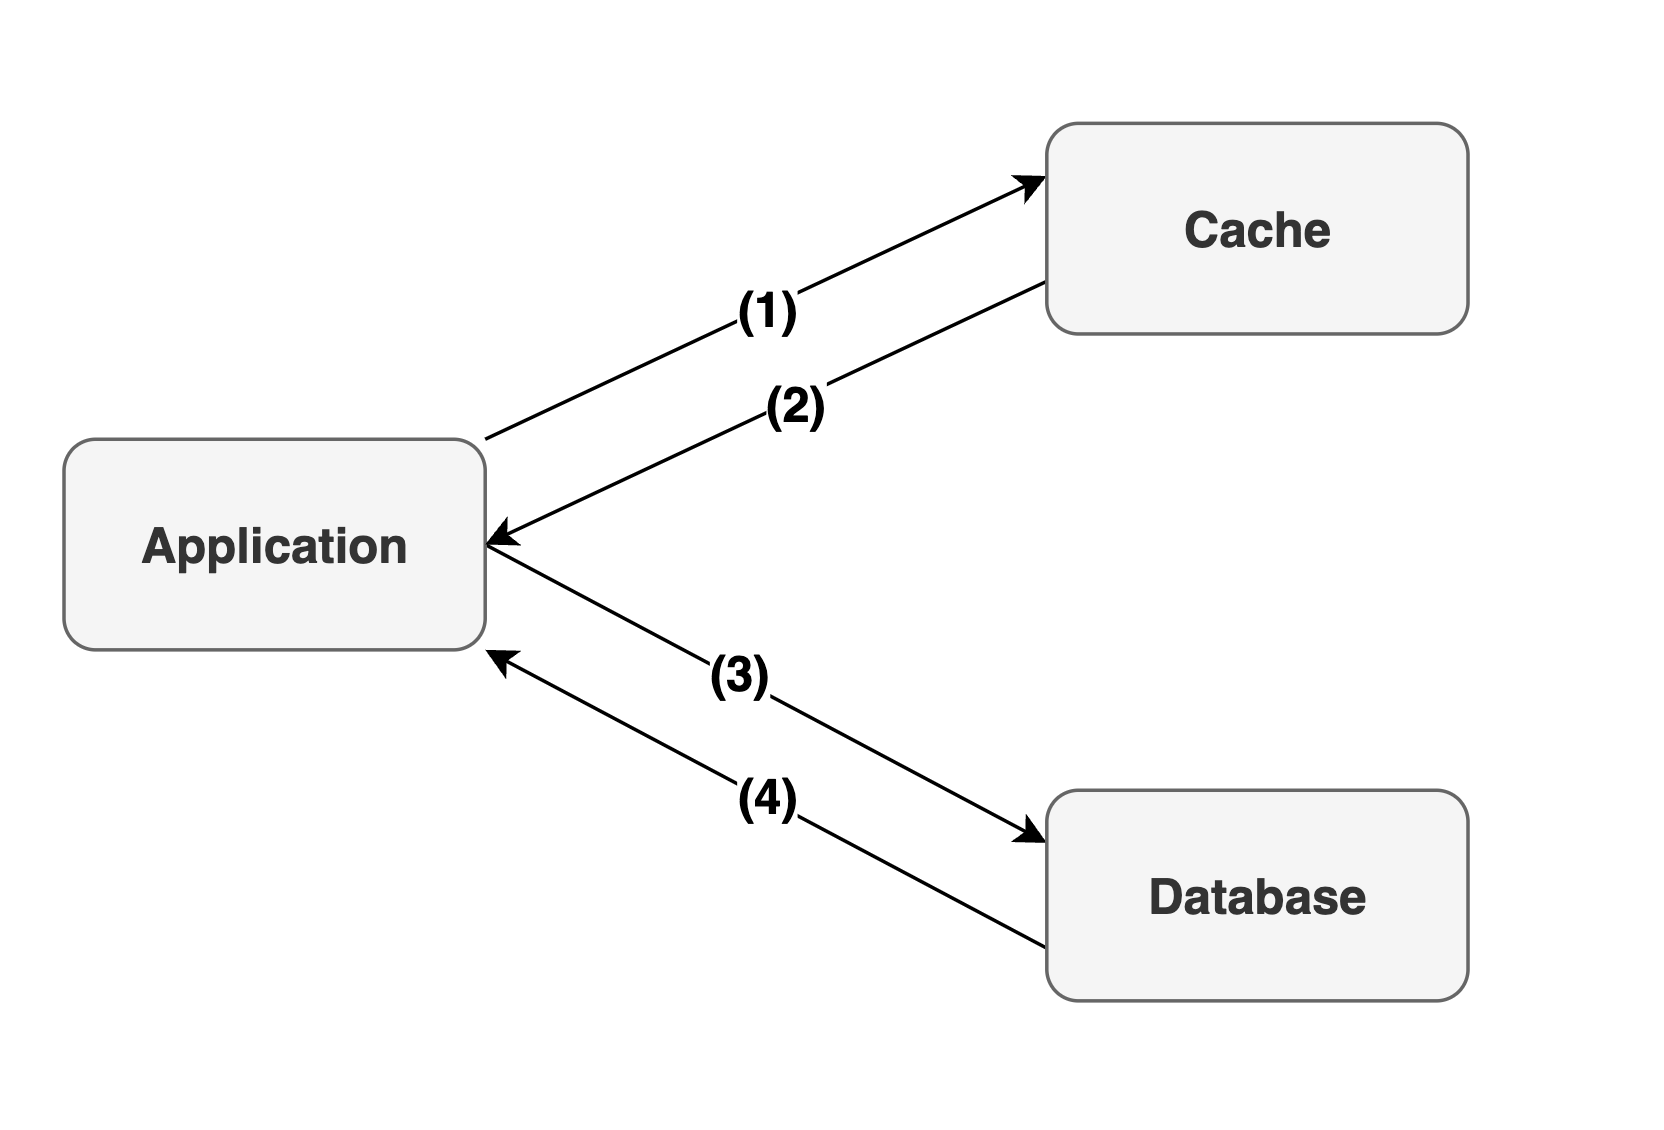
\includegraphics[width=0.8\textwidth]{Figures/caching_strat.png}
    \caption{Caching Mechanism}
\end{figure}

\section{Advanced search strategy}

Querying data that requires applying many filters (pet profiles, etc)
from the SQL database is extremely time-consuming. Note that only data
that is used repeatedly and is not too large in size can be stored
temporarily in the cache server. Therefore, applying a search strategy
to optimize querying the above type of data is necessary.

\emph{Figure 5.2} shows the steps of syncing data from the SQL database
to the Elastic-search database.

\begin{itemize}
    \item
          Whenever the application does an action on a record of the SQL
          database (create, update, delete), a new record (which includes the ID
          of the record taken the action, and the action), from now we call the
          async record, is created.
    \item
          At the end of the application process, a background job is triggered
          to query all the async records and send all the records that they
          point to onto the Elastic-search database. Therefore the data of the
          Elastic-search database is always synchronized with the SQL database.
    \item
          Note that the application only queries data from the Elastic-search
          database for tables that were defined before.
\end{itemize}

\begin{figure}[H]
    \centering
    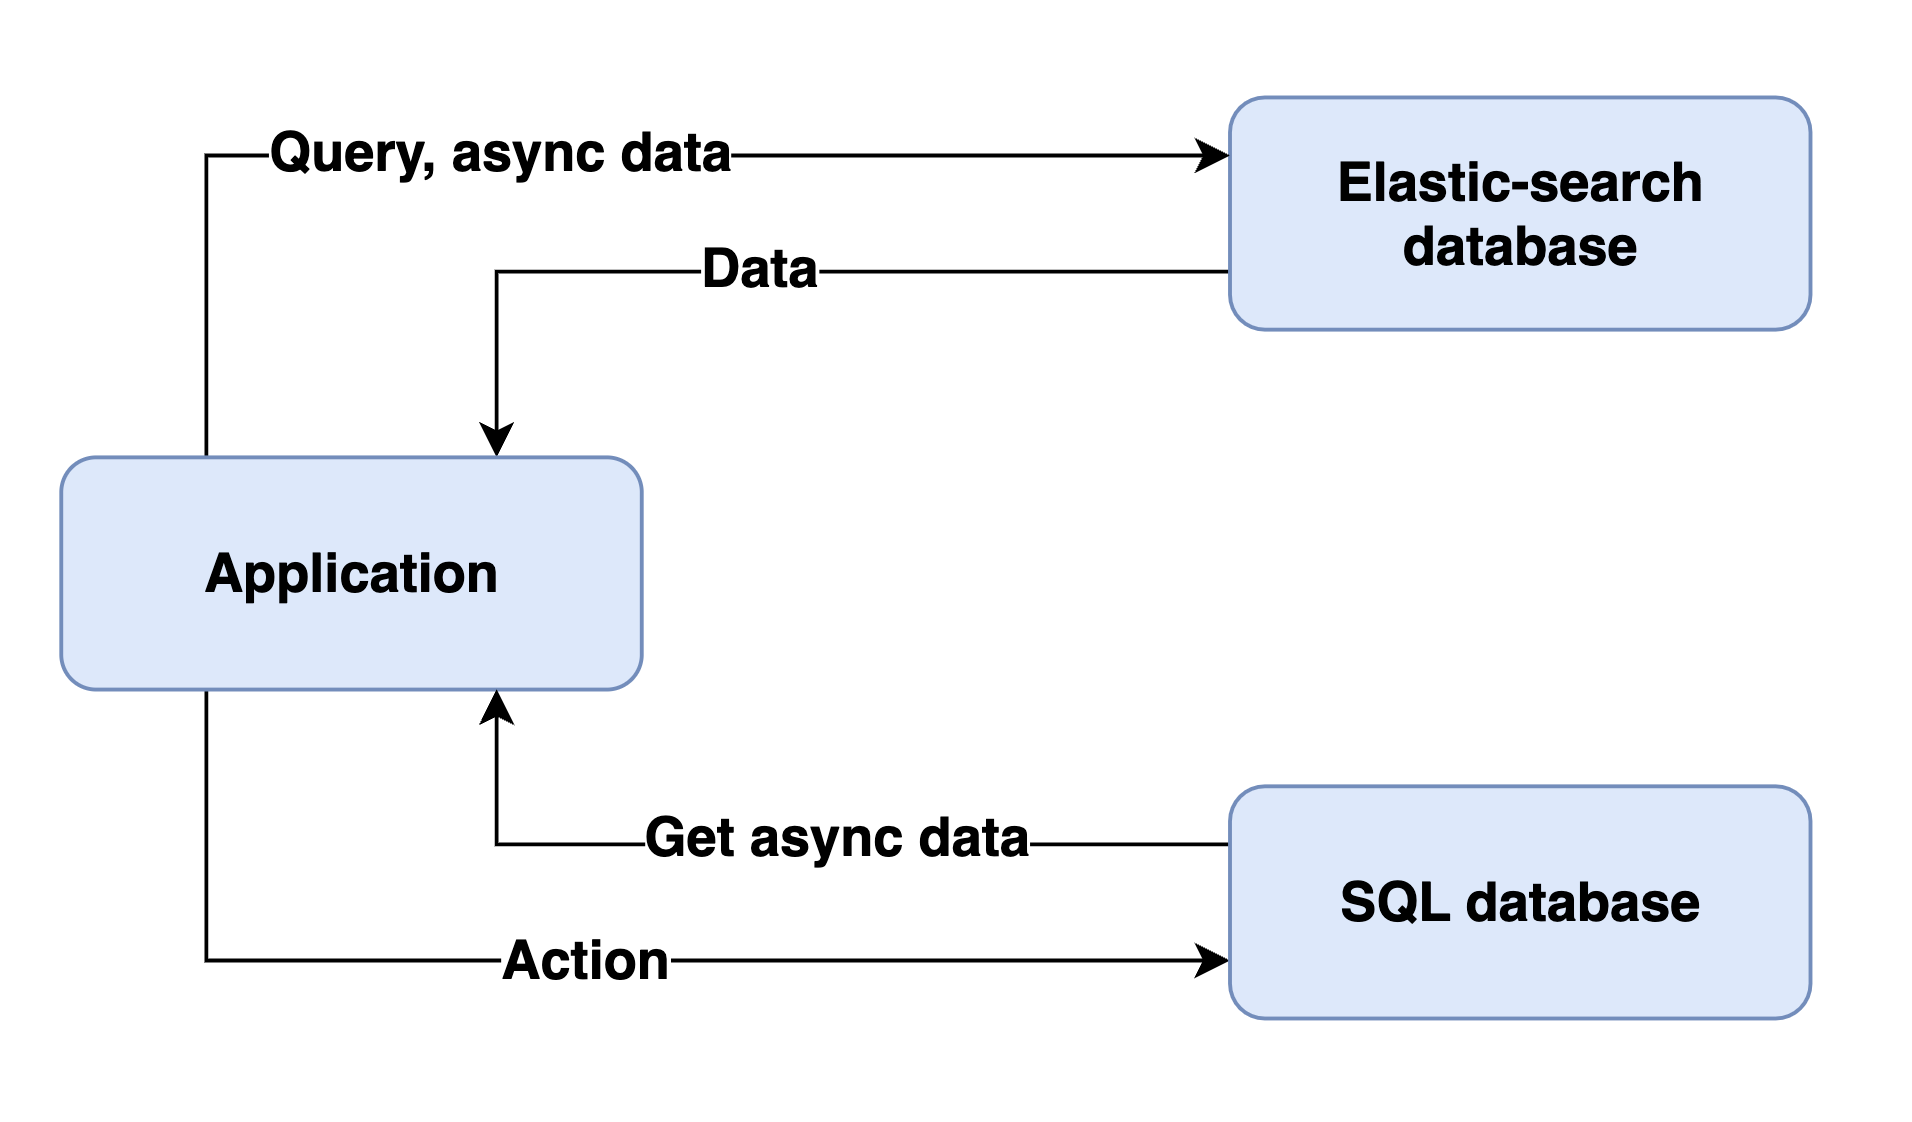
\includegraphics[width=0.8\textwidth]{Figures/search_strat.png}
    \caption{Search strategy}
\end{figure}

\section{Online payment}

In our system, we have integrated the PayPal Braintree Gateway to handle online payments securely and efficiently. Braintree is a full-stack payment platform that offers a seamless payment experience, supporting various payment methods, including credit cards, PayPal, and other digital wallets. Its robust infrastructure and comprehensive SDKs for both client and server sides make it an ideal choice for our system's payment processing needs.

\begin{figure}[H]
    \centering
    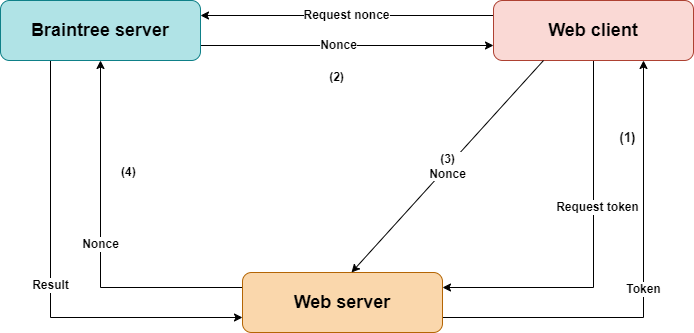
\includegraphics[width=0.7\textwidth]{Figures/payment-strat.png}
    \caption{Payment process}
\end{figure}

\emph{Figure 5.3} breaks down how the payment process is implemented:

- Step 1:
The front-end requests a client token from our server and initializes the Braintree client. This token is essential for securely communicating between the client and the Braintree server.\\
Our server generates a client token using Braintree's tools and sends it back to the client. This token allows the front-end to securely handle customer payment information.

- Step 2:
The customer enters their payment information on the front-end. The Braintree client communicates this information to Braintree and returns a payment method nonce, a secure reference representing the payment details.

- Step 3:
The front-end sends the payment method nonce to our server. This nonce is a secure way to pass payment information without exposing sensitive data.

- Step 4:
The server receives the payment method nonce and uses Braintree's tools to process the payment. The server then communicates with Braintree to complete the transaction securely.

By utilizing PayPal Braintree Gateway, we ensure a secure and streamlined payment process, enhancing the user experience and maintaining high security standards in handling sensitive payment information.

\section{Google Login}
Our website provides users with the option to log in using their Google account, 
offering a convenient and secure authentication method. By integrating Google Sign-In, 
we simplify the login process for users and enhance the overall user experience. 

The Google Login process is illustrated in \emph{Figure 5.4}:
\begin{figure}[H]
    \centering
    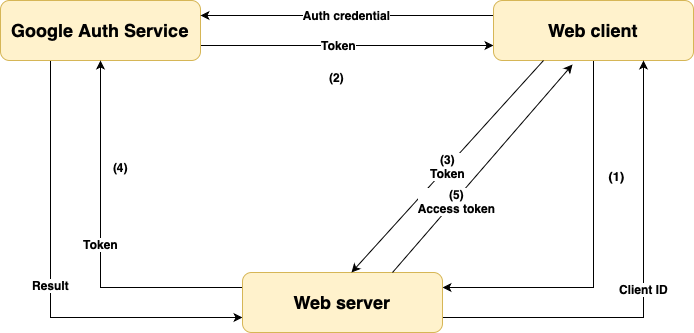
\includegraphics[width=0.7\textwidth]{Figures/Implementation/GoogleLogin.png}
    \caption{Google Login Process}
\end{figure}

The implementation steps are as follows:
\begin{itemize}
    \item Step 1: The web client obtains the client ID from the web server.
    \item Step 2: When the user clicks the Google login button, the web client displays the Google Login form. The user logs in using their Google account, and Google generates a token, which is sent back to the web client.
    \item Step 3: The web client sends the token to the web server.
    \item Step 4: The web server verifies the token with Google. If the token is valid, Google confirms this to the web server.
    \item Step 5: The web server creates an access token and sends it back to the web client. The user can now access the website using this access token.
\end{itemize}

\section{Breeds Recognition}
Breed recognition is a valuable feature for our users, who often don't know their pet's breed. To address this, we utilized ML.NET 
to train an image classification model. This advanced technology enables our platform to accurately identify a pet's breed from a photo, 
simplifying the process for users and enhancing their experience.

The first step is preparing the dataset. We have chosen the Stanford Dogs dataset\footnote{Stanford Dogs dataset: \url{https://www.kaggle.com/datasets/jessicali9530/stanford-dogs-dataset}}, which contains images of 120 dog breeds from around 
the world. This dataset, built using images and annotations from ImageNet, is ideal for the task of fine-grained image categorization. 
The challenging nature of this problem stems from the fact that certain dog breeds have nearly identical features or differ only in color and age.

For cat breed classification, we use the Cat Breeds Dataset (Cleared)\footnote{Cat Breeds Dataset (Cleared): \url{https://www.kaggle.com/datasets/denispotapov/cat-breeds-dataset-cleared}}, which contains images of 67 different cat breeds, labeled by advertisers for 
adoption. This dataset is a refined version of the original Cat Breeds Dataset from Kaggle \footnote{Stanford Dogs dataset: \url{https://www.kaggle.com/ma7555/cat-breeds-dataset}}. 
The cleared version has been meticulously cleaned to remove non-cat images, indistinguishable cat photos, duplicates, and very small images 
(height or width less than 150 pixels). This ensures that the dataset is of high quality, facilitating accurate training and performance of our 
machine learning model.

The images in the dataset are organized into separate folders for each dog breed, simplifying the model training process. This organization 
makes it more convenient to manage and feed the data into our machine learning model. Using this well-structured dataset, we can effectively 
train our image classification model with ML.NET to recognize and categorize various dog breeds accurately.

The next step involves using ML.NET Model Builder to transform our image set into an image classification model. Here's how we proceed:
\begin{enumerate}
    \item Load the Data: Import the cleaned datasets for dog and cat breeds into the ML.NET Model Builder. These datasets include images 
    categorized into folders based on their respective breeds.
    \item Set Up the Environment: Configure the Model Builder environment on our local machine, ensuring that all necessary tools and dependencies are installed.
    \item Select the Scenario: Choose the 'Image Classification' scenario in ML.NET Model Builder, which is specifically designed for tasks like breed recognition.
    \item Train the Model:
    \begin{itemize}
        \item Data Preprocessing: The Model Builder automatically preprocesses the images, resizing and normalizing them as required.
        \item Model Selection and Training: The tool selects a suitable pre-trained model and fine-tunes it using our dataset. This involves 
        splitting the data into training and validation sets to ensure the model learns effectively and generalizes well.
        \item Local Training: The model is trained on our local machine, leveraging available computational resources to iterate through 
        the dataset and optimize the classification accuracy.
    \end{itemize}
    \item Evaluate the Model: Once training is complete, the Model Builder evaluates the model's performance, 
    providing metrics such as accuracy, precision, recall, and F1 score. This helps in understanding how well 
    the model distinguishes between different breeds.

    After training the model for dog breed recognition, we evaluated its performance using various algorithms. 
    The micro-accuracy algorithm identified the best model, achieving a micro-accuracy score of 0.8345. This 
    high accuracy indicates that the model can reliably recognize and classify different dog breeds, providing 
    users with accurate breed identification based on their pet's images.

    \begin{figure}[H]
        \centering
        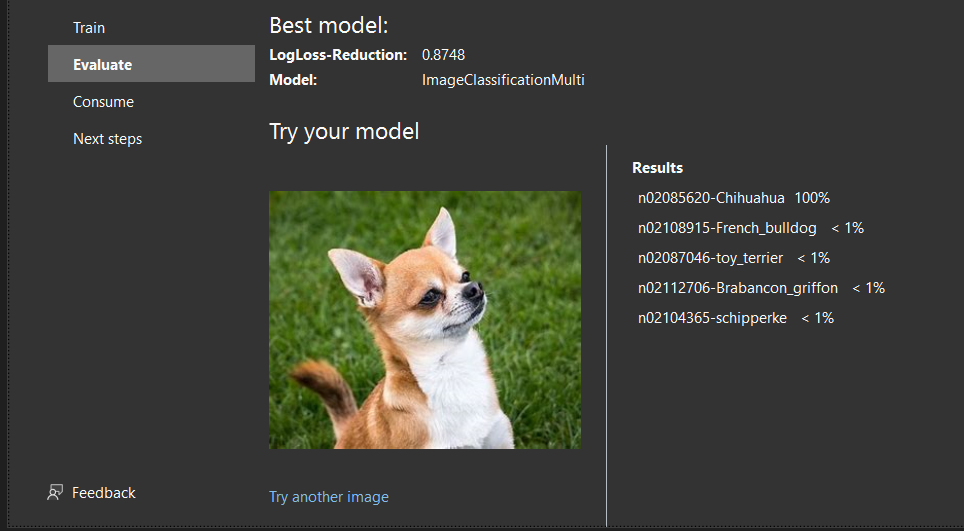
\includegraphics[width=0.7\textwidth]{Figures/AI/ai_result.png}
        \caption{Results of Dog Breed Recognition}
    \end{figure}

    For cat breed recognition, we followed a similar process, training the model on the Cat Breeds Dataset (Cleared)
    and evaluating its performance. The micro-accuracy algorithm identified the best model, achieving a micro-accuracy
    score of 0.4321. This indicates that the dataset is more challenging for cat breed recognition, as the model's accuracy
    is lower compared to dog breed recognition. Despite this, the model can still classify cat breeds with reasonable accuracy,
    providing users with valuable insights into their pet's breed based on images. 

    \item Export the Model: Finally, the trained model is exported for integration into our application. 
    The Model Builder generates the necessary code and files, making it straightforward to deploy the model.
    In our case, we export the model as an API, allowing seamless integration with our platform for real-time breed recognition.
\end{enumerate}

\section{Protect System APIs with Access/Refresh Tokens}
To authenticate users and authorize requests without keeping session data on the server, we use \textit{tokens}, which are data confirming a user’s identity and are analogous to digital signatures.

A careful balance between security and user experience is essential for authentication and authorization. A user may become irritated if protocols are overly strict. On the other hand, a security breach is imminent if permission systems are too loose. Access and refresh tokens provide a solution that meets both requirements.

\textbf{An access token} allows temporary access to restricted resources such as APIs or websites. The chance of the access token being compromised or stolen increases the longer it’s valid. Therefore, access tokens are valid for only \textit{a few minutes or hours}.

\textbf{An refresh token} allow developers to manage users’ sessions across the application. Additionally, they allow users to log in and stay connected without providing their passwords for long periods. Therefore, refresh tokens can last \textit{from a few days to a few months}.

Let’s now discuss how to set up the tokens in \textit{Figure 5.6}:

\begin{figure}[H]
  \centering
  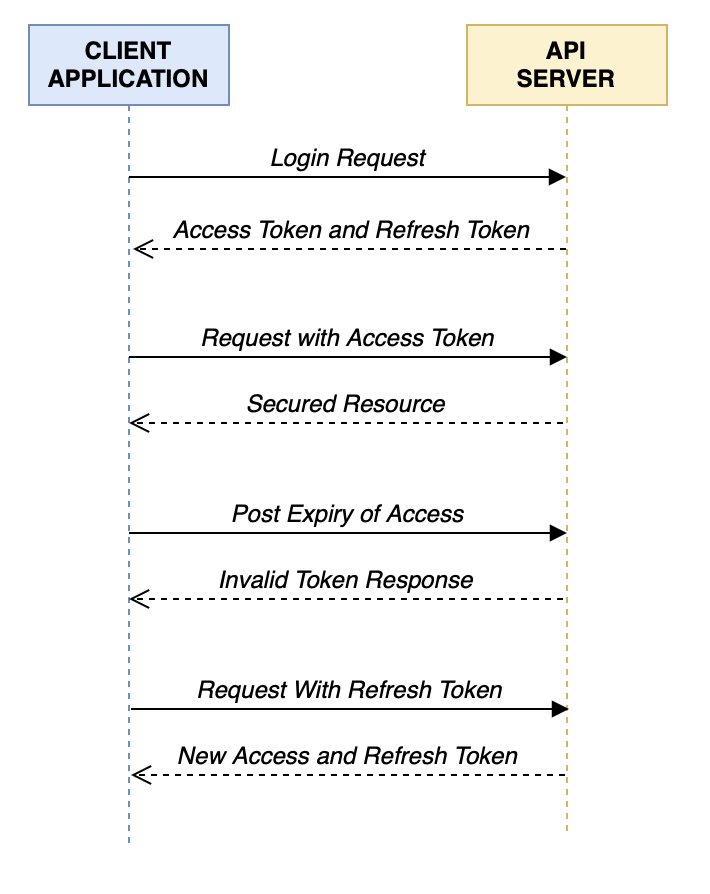
\includegraphics[width=0.6\textwidth]{Figures/Implementation/Tokens.png}
  \caption{Set up the tokens.}
\end{figure}

Let’s say a client requests an access token by authenticating with the authorization server and delivering a credential that proves the resource owner is authorized to use the resource.

The API server verifies the authorization and confirms the identity of the authorized client. An access token and a refresh token are issued if it’s legitimate. The client must securely store this refresh token.

The client can now request the API server for secured resource access, and the resource server validates the access token. If it’s valid, it returns the desired resource.
\chapter{SYSTEM TESTING}

With the completion of system implementation, our focus now shifts towards ensuring the robustness and functionality of the system through testing. This section presents the systematic approach taken for system testing, including end-to-end testing, API testing, load testing, and performance testing to validate the functionality and performance of the implemented system

\section{API testing}
This section delves into testing the website's API for functionality using 
Postman. Postman's versatile features were utilized to conduct thorough 
assessments of the API endpoints, ensuring data integrity and performance 
across diverse scenarios. Through rigorous experimentation and analysis, 
Postman facilitated the establishment of a robust validation framework, 
affirming the reliability of the website's API under different conditions.

\subsection{API endpoints}
The website's API endpoints were meticulously tested to ensure their
functionality and performance across various scenarios. The API endpoints
were designed to handle different types of requests, including GET, POST,
PUT, and DELETE, to interact with the database and retrieve or modify
data. By testing these endpoints, we could verify the accuracy and
reliability of the API, ensuring that it could handle different types of
requests and return the expected results.

\subsection{Automation API Testing with Postman}
Postman was used to test the website's API endpoints, leveraging its
versatile features to conduct comprehensive assessments. Postman's
user-friendly interface and powerful testing capabilities enabled us to
create test-cases, execute requests, and analyze responses efficiently.
By defining test scripts and assertions, we could validate the API
endpoints' functionality and performance, ensuring that they met the
specified requirements.
In this section, we focus on the response data, status code, and response
time of the API endpoints, evaluating their accuracy and reliability.
For status, we have this code on Postman
\begin{lstlisting}[caption=Code to test status code, label={lst:status-code}]
    pm.test("Status code is 200", function () {
        pm.response.to.have.status(200);
    });
\end{lstlisting}
To test the status code, we used the following code in Postman:
\begin{lstlisting}[caption=Code to test response time, label={lst:response-time}]
    pm.test("Response time is less than 200ms", function () {
        pm.expect(pm.response.responseTime).to.be.below(200);
    });
\end{lstlisting}
To test the response data, we used this code in Postman:
\begin{lstlisting}[caption=Code to test response data, label={lst:response-data}]
    pm.test("Response contains errorCode: 10006 and errorMessage: Wrong login type", function () {
    var responseData = pm.response.json();
    pm.expect(responseData).to.eql({ errorCode: 10006, errorMessage: "Wrong login type" });
});
\end{lstlisting}

\subsection{API Testing Test-cases}
Various testing scenarios were explored to evaluate the website's API
endpoints thoroughly. These scenarios included testing different types of
requests, handling error conditions, and assessing the API's performance
under load. By simulating real-world usage scenarios and edge cases, we
could identify potential issues and validate the API's behavior in
different situations. This comprehensive testing approach helped ensure
the reliability and robustness of the website's API, enhancing its overall
quality and performance. 

Here is all the test-cases for the API endpoints. All the API endpoints
here have average response time of 734ms. The test-cases are divided into:


\begin{longtblr}[
    caption = {API Testing for Adoption Form},
    label = {tblr:api_adoption_form},
  ]{
    hlines, vlines,
    colspec = {X[0.5,l] X[3,l] X[4,l] X[5,l] X[1.5,l] X[2,l]},
    row{1} = {font=\bfseries},
  }
  Id                & Api                                          & Testcase               & Expected result                                                             & Result & \SetCell[c=1]{c}Response time \\
  \SetCell[r=3]{c}1 & \SetCell[r=3]{c}POST - /AdoptionForm         & 1. Unauthorized        & Error code 400 with message "Unauthorized".                                 & Pass   & \SetCell[r=3]{c}872ms         \\
                    &                                              & 2. Empty body          & Error code 401 with corresponding empty fields.                             & Pass   &                               \\
                    &                                              & 3. Correct body        & Status 200.                                                                 & Pass                                   \\
  \SetCell[r=3]{c}2 & \SetCell[r=3]{c}GET - /AdoptionForm/ Precheck & 1. Is adopted          & Error code 12003 with message "You have sent request for this pet already". & Pass   & \SetCell[r=3]{c}812ms         \\
                    &                                              & 2. Not adopted         & Success with status 200                                                     & Pass   &                               \\
                    &                                              & 3. Adopt from yourself & Error code 12002 with message "Can not adopt your own pet"                  & Pass   &                               \\
  \SetCell[r=2]{c}3 & \SetCell[r=2]{c}GET - /AdoptionForm/Incoming & 1. Unauthorized        & Error code 400 with message "Unauthorized".                                 & Pass   & \SetCell[r=2]{c}527ms         \\
                    &                                              & 2. Authorized          & Success with status 200                                                     & Pass   &                               \\
  \SetCell[r=2]{c}4 & \SetCell[r=2]{c}GET - /AdoptionForm/Sent     & 1. Unauthorized        & Error code 400 with message "Unauthorized".                                 & Pass   & \SetCell[r=2]{c}644ms         \\
                    &                                              & 2. Authorized          & Success with status 200                                                     & Pass   &                               \\
  \SetCell[r=2]{c}5 & \SetCell[r=2]{c}GET - /CountUnreadIncoming   & 1. Unauthorized        & Error code 400 with message "Unauthorized".                                 & Pass   & \SetCell[r=2]{c}613ms         \\
                    &                                              & 2. Authorized          & Success with status 200                                                     & Pass   &                               \\
\end{longtblr}

\begin{longtblr}[
        caption = {API Testing for Authentication Function},
        label = {tblr:api_Authentication},
    ]{
        hlines, vlines,
        colspec = {X[0.5,l] X[3,l] X[4,l] X[5,l] X[1.5,l] X[2,l]},
        row{1} = {font=\bfseries},
    }
    Id                & Api                                             & Testcase             & Expected result                                       & Result & \SetCell[c=1]{c}Response time \\
    \SetCell[r=3]{c}1 & \SetCell[r=3]{c}POST - /Authentication/Register & 1. Empty body        &                                                       & Pass   & \SetCell[r=3]{c}637ms         \\*
                      &                                                 & 2. Email is used     &                                                       & Pass   &                               \\
                      &                                                 & 3. Email is not used &                                                       & Pass   &                               \\
    \SetCell[r=5]{c}2 & \SetCell[r=5]{c}POST - /Authentication/Login    & 1. Wrong email       & Error code 10001 with message "Invalid credential".   & Pass   & \SetCell[r=5]{c}669ms         \\*
                      &                                                 & 2. Wrong password    & Error code 10001 with message "Invalid credential".   & Pass   &                               \\
                      &                                                 & 3. Correct account   & Status 200.                                           & Pass   &                               \\
                      &                                                 & 4. Wrong login type  & Error code 10006 with message "Wrong login type".     & Pass   &                               \\
                      &                                                 & 5. Empty body        & Error code 400 with corresponding empty fields        & Pass   &                               \\
    \SetCell[r=2]{c}3 & GET - /Authentication/-Logout                   & 1. Unauthorized      & Error code 401 with message "Unauthorized".           & Pass   & \SetCell[r=2]{c}838ms         \\*
                      &                                                 & 2. Authorized        & Status 200.                                           & Pass   &                               \\
    \SetCell[r=2]{c}4 & \SetCell[r=2]{c}GET - /Authentication/Refresh   & 1. Unauthorized      & Error code 401 with message "Invalid security token". & Pass   & \SetCell[r=2]{c}750ms         \\*
                      &                                                 & 2. Authorized        & Status 200.                                           & Pass   &                               \\
\end{longtblr}

\begin{longtblr}[
    caption = {API Testing for Blog Function},
    label = {tblr:api_Blog},
  ]{
    hlines, vlines,
    colspec = {X[0.5,l] X[3,l] X[4,l] X[5,l] X[1.5,l] X[2,l]},
    row{1} = {font=\bfseries},
  }
  Id                & Api                                         & Testcase                   & Expected result                                 & Result & Response time         \\
  \SetCell[r=4]{c}1 & \SetCell[r=4]{c}POST - /Blog                & 1. Unauthorized            & Error code 401 with message "Unauthorized".     & Pass   & \SetCell[r=4]{c}693ms \\*
                    &                                             & 2. Wrong role              & Error code 400 with message "Forbidden".        & Pass   &                       \\
                    &                                             & 3. Correct body            & Status 200.                                     & Pass   &                       \\
                    &                                             & 4. Empty body              & Error code 400 with corresponding empty fields. & Pass   &                       \\
  \SetCell[r=4]{c}2 & \SetCell[r=4]{c}PUT - /Blog                 & 1. Unauthorized            & Error code 401 with message "Unauthorized".     & Pass   & \SetCell[r=4]{c}700ms \\*
                    &                                             & 2. Wrong role              & Error code 400 with message "Forbidden".        & Pass   &                       \\
                    &                                             & 3. Correct body            & Status 200.                                     & Pass   &                       \\
                    &                                             & 4. Empty body              & Error code 400 with corresponding empty fields. & Pass   &                       \\
  \SetCell[r=2]{c}3 & \SetCell[r=2]{c}POST - /Blog/Get            & 1. Empty body              & Response with status 500.                       & Pass   & \SetCell[r=2]{c}681ms \\*
                    &                                             & 2. Correct body            & Status 200.                                     & Pass   &                       \\
  \SetCell[r=4]{c}4 & \SetCell[r=4]{c}DELETE - /Blog/\{blog\_id\} & 1. Unauthorized            & Error code 401 with message "Unauthorized".     & Pass   & \SetCell[r=4]{c}677ms \\*
                    &                                             & 2. Delete existed blog     & Success with status 200.                        & Pass   &                       \\
                    &                                             & 3. Delete non-existed blog & Error code 400 with message "Forbidden".        & Pass   &                       \\
                    &                                             & 4. Delete empty blog\_id   & Error with status 405.                          & Pass   &                       \\
  \SetCell[r=3]{c}5 & \SetCell[r=3]{c}POST - /Blog/User           & 1. Unauthorized            & Error code 401 with message "Unauthorized".     & Pass   & \SetCell[r=3]{c}667ms \\*
                    &                                             & 2. Empty body              & Response with status 500.                       & Pass   &                       \\
                    &                                             & 3. Correct body            & Status 200.                                     & Pass   &                       \\
\end{longtblr}


\begin{longtblr}[
    caption = {API Testing for Comment Function},
    label = {tblr:api_comment},
  ]{
    hlines, vlines,
    colspec = {X[0.5,l] X[3,l] X[4,l] X[5,l] X[1.5,l] X[2,l]},
    row{1} = {font=\bfseries},
  }
  Id                & Api                                              & Testcase                 & Expected result                                               & Result & \SetCell[c=1]{c}Response time \\
  \SetCell[r=3]{c}1 & \SetCell[r=3]{c}GET - /Comment/blog/\{blog\_id\} & 1. Correct id            & Status 200                                                    & Pass   & \SetCell[r=3]{c}708ms         \\
                    &                                                  & 2. Wrong blog id         & Status 400 with message "The value \{blog\_id\} id not valid" & Pass   &                               \\
                    &                                                  & 3. Empty blog id         & Status 405                                                    & Pass   &                               \\
  \SetCell[r=3]{c}2 & \SetCell[r=3]{c}GET - /Comment/post/\{blog\_id\} & 1. Correct id            & Status 200                                                    & Pass   & \SetCell[r=3]{c}629ms         \\
                    &                                                  & 2. Wrong blog id         & Status 400 with message "The value \{blog\_id\} id not valid" & Pass   &                               \\
                    &                                                  & 3. Empty blog id         & Status 405                                                    & Pass   &                               \\
  \SetCell[r=3]{c}3 & \SetCell[r=3]{c}POST - /Comment                  & 1. Unauthorized          & Error code 401 with message "Unauthorized".                   & Pass   & \SetCell[r=3]{c}779ms         \\
                    &                                                  & 2. Comment with text     & Status 200.                                                   & Pass   &                               \\
                    &                                                  & 3. Empty comment         & Error code 401 with message "Can not be empty".               & Pass   &                               \\
  \SetCell[r=3]{c}4 & \SetCell[r=3]{c}DEL - /Comment/ \{comment\_id\}   & 1. Unauthorized          & Error code 401 with message "Unauthorized".                   & Pass   & \SetCell[r=3]{c}697ms         \\
                    &                                                  & 2. Delete self comment   & Status 200.                                                   & Pass   &                               \\
                    &                                                  & 3. Delete others comment & Error code 401 with message "Unauthorized".                   & Pass   &                               \\
\end{longtblr}

\begin{longtblr}[
    caption = {API Testing for Location Function},
    label = {tblr:api_location},
  ]{
    hlines, vlines,
    colspec = {X[0.5,l] X[3,l] X[4,l] X[5,l] X[1.5,l] X[2,l]},
    row{1} = {font=\bfseries},
  }
    Id & Api & Testcase & Expected result & Result & \SetCell[c=1]{c}Response time \\
    \SetCell[r=8]{c}1 & \SetCell[r=8]{c}GET - /Location & 1. Unauthorized & Error code 401 with message "Unauthorized". & Pass & \SetCell[r=8]{c}707ms \\
    & & 2. Empty level and code & Status 200 with empty data & Pass & \\
    & & 3. Level = 1 & Return all provinces & Pass & \\
    & & 4. Level = 2 & Status 200 with empty data & Pass & \\
    & & 5. Code = 1 & Status 200 with empty data & Pass & \\
    & & 6. Level = 2, Code = 79 & Return all districts corresponding to level & Pass & \\
    & & 7. Level = 3, Code = 775 & Return all wards corresponding to level & Pass & \\
    & & 8. Level = wrong, Code = wrong & Status 400 with message "The value 'wrong' is not valid for level" & Pass & \\
  \end{longtblr}

\begin{longtblr}[
    caption = {API Testing for Notification Function},
    label = {tblr:api_notification},
  ]{
    hlines, vlines,
    colspec = {X[0.6,l] X[2.3,l] X[3.3,l] X[4.5,l] X[0.8,l] X[1.7,l]},
    row{1} = {font=\bfseries},
  }
    Id & Api & Testcase & Expected result & Result & \SetCell[c=1]{c}Response time \\
    1 & GET - /Notification & 1. Unauthorized & Error code 401 with message "Unauthorized". & Pass & 651ms \\
    & & 2. Authorize & Status 200 with message "true" & Pass & \\
    \SetCell[r=2]{c}2 & \SetCell[r=2]{c}DEL - /Notification & 1. Unauthorized & Error code 401 with message "Unauthorized". & Pass & \SetCell[r=2]{c}678ms \\
    & & 2. Authorize & Status 200 with message "true" & Pass & \\
    \SetCell[r=3]{c}3 & \SetCell[r=3]{c}PUT - /Notification/\{notification\_id\} & 1. Unauthorized & Error code 401 with message "Unauthorized". & Pass & \SetCell[r=3]{c}685ms \\
    & & 2. Update others comment & Status 200 with message "false" & Pass & \\
    & & 3. Update self comment & Status 200 with message "true" & Pass & \\
  \end{longtblr}

\begin{longtblr}[
    caption = {API Testing for Payment Function},
    label = {tblr:api_payment},
  ]{
    hlines, vlines,
    colspec = {X[0.5,l] X[3,l] X[4,l] X[5,l] X[1.5,l] X[2,l]},
    row{1} = {font=\bfseries},
  }
    Id & Api & Test-case & Expected result & Result & \SetCell[c=1]{c}Response time \\
    \SetCell[r=3]{c}1 & \SetCell[r=3]{c}GET - /Payment/Token & 1. Unauthorized & Error code 401 with message "Unauthorized". & passed & \SetCell[r=3]{c}617ms \\*
    & & 2. Wrong role & Status 400 with message "Forbidden" & passed & \\
    & & 3. Correct role & Status 200 & passed & \\
    \SetCell[r=2]{c}2 & \SetCell[r=2]{c}POST - /Payment & 1. Unauthorized & Error code 401 with message "Unauthorized". & passed & \SetCell[r=2]{c}648ms \\*
    & & 2. Wrong role & Status 400 with message "Forbidden" & passed & \\
    \SetCell[r=3]{c}3 & \SetCell[r=3]{c}GET - /Payment/AdvertisementType & 1. Unauthorized & Error code 401 with message "Unauthorized". & passed & \SetCell[r=3]{c}666ms \\*
    & & 2. Wrong role & Status 400 with message "Forbidden" & passed & \\
    & & 3. Correct role & Status 200 & passed & \\
  \end{longtblr} 

\begin{longtblr}[
    caption = {API Testing for Pet Function},
    label = {tblr:api_pet},
  ]{
    hlines, vlines,
    colspec = {X[0.5,l] X[3,l] X[4,l] X[5,l] X[1.5,l] X[2,l]},
    row{1} = {font=\bfseries},
  }
    Id & Api & Test-case & Expected result & Result & \SetCell[c=1]{c}Response time \\
    \SetCell[r=3]{c}1 & \SetCell[r=3]{c}POST - /Pet & 1. Unauthorized & Error code 401 with message "Unauthorized". & passed & \SetCell[r=3]{c}620ms \\*
    & & 3. Correct body & Status 200. & passed & \\
    & & 4. Empty body & Error code 400 with corresponding empty fields & passed & \\
    \SetCell[r=4]{c}2 & \SetCell[r=4]{c}PUT - /Pet & 1. Unauthorized & Error code 401 with message "Unauthorized". & passed & \SetCell[r=4]{c}723ms \\*
    & & 2. Wrong field value & Error status 400 & passed & \\
    & & 3. Correct body & Status 200. & passed & \\
    & & 4. Empty body & Error code 400 with corresponding empty fields & passed & \\
    \SetCell[r=9]{c}3 & \SetCell[r=9]{c}POST - /Pet/Get & 1. Unauthorized & Error code 401 with message "Unauthorized". & passed & \SetCell[r=9]{c}757ms \\*
    & & 2. Empty body & Error code 400 with corresponding empty fields & passed & \\
    & & 3. Test filter species & Response contains pet with correct species & passed & \\
    & & 4. Test filter sex & Response contains pet with correct sex & passed & \\
    & & 5. Test filter age & Response contains pet with correct age & passed & \\
    & & 6. Test filter color & Response contains pet with correct color & passed & \\
    & & 7. Test filter size & Response contains pet with correct size & passed & \\
    & & 8. Test filter isSterilized & Response contains pet with correct isSterilized & passed & \\
    & & 9. Test filter Vaccinated & Response contains pet with correct Vaccinated & passed & \\
    \SetCell[r=3]{c}4 & \SetCell[r=3]{c}DELETE - /Pet/\{pet\_id\} & 1. Unauthorized & Error code 401 with message "Unauthorized". & passed & \SetCell[r=3]{c}719ms \\*
    & & 2. Delete existing pet & Success with status 200 & passed & \\
    & & 3. Delete non-existing pet & Error code 11001 with message "The pet is not found". & passed & \\
  \end{longtblr}


\begin{longtblr}[
    caption = {API Testing for Report Function},
    label = {tblr:api_report},
  ]{
    hlines, vlines,
    colspec = {X[0.5,l] X[3,l] X[4,l] X[5,l] X[1.5,l] X[2,l]},
    row{1} = {font=\bfseries},
  }
    Id & Api & Testcase & Expected result & Result & \SetCell[c=1]{c}Response time \\
    \SetCell[r=8]{c}1 & \SetCell[r=8]{c}{POST - /Report/PreReport} & 1. Unauthorized & Error code 401 with message "Unauthorized". & Pass & \SetCell[r=8]{c}679ms \\*
    & & 2. Report yourself & Status 200 with message "false" & Pass & \\
    & & 3. Report other user & Status 200 with message "true" & Pass & \\
    & & 4. Report other user with wrong entity & Status 200 with message "false" & Pass & \\
    & & 5. Report your blog & Status 200 with message "false" & Pass & \\
    & & 6. Report others' blog & Status 200 with message "true" & Pass & \\
    & & 7. Report your pet & Status 200 with message "false" & Pass & \\
    & & 8. Report others' pet & Status 200 with message "true" & Pass & \\
    \SetCell[r=8]{c}2 & \SetCell[r=8]{c}{POST - /Report/Report} & 1. Unauthorized & Error code 401 with message "Unauthorized". & Pass & \SetCell[r=8]{c}733ms \\*
    & & 2. Report yourself & Status 200 with message "false" & Pass & \\
    & & 3. Report other user & Status 200 with message "true" & Pass & \\
    & & 4. Report other user with wrong entity & Status 200 with message "false" & Pass & \\
    & & 5. Report your blog & Status 200 with message "true" & Pass & \\
    & & 6. Report others' blog & Status 200 with message "true" & Pass & \\
    & & 7. Report your pet & Status 200 with message "false" & Pass & \\
    & & 8. Report others' pet & Status 200 with message "true" & Pass & \\
  \end{longtblr}

\begin{longtblr}[
    caption = {API Testing for User Function},
    label = {tblr:api_user},
  ]{
    hlines, vlines,
    colspec = {X[0.5,l] X[3,l] X[4,l] X[5,l] X[1.5,l] X[2,l]},
    row{1} = {font=\bfseries},
  }
  Id                & Api                                         & Testcase            & Expected result                                               & Result & \SetCell[c=1]{c}Response time \\
  \SetCell[r=2]{c}1 & \SetCell[r=2]{c}GET - /User/CurrentUser     & 1. Unauthorized     & Error code 401 with message "Unauthorized".                   & Pass   & \SetCell[r=2]{c}694ms         \\*
                    &                                             & 2. Authorized       & Status 200.                                                   & Pass   &                               \\
  \SetCell[r=2]{c}2 & \SetCell[r=2]{c}GET - /User/CurrentUserCore & 1. Unauthorized     & Error code 401 with message "Unauthorized".                   & Pass   & \SetCell[r=2]{c}884ms         \\*
                    &                                             & 2. Authorized       & Status 200.                                                   & Pass   &                               \\
  \SetCell[r=2]{c}3 & \SetCell[r=2]{c}GET - /User/ OtherUser       & 1. Unauthorized     & Status 200.                                                   & Pass   & \SetCell[r=2]{c}664ms         \\*
                    &                                             & 2. Authorized       & Status 200.                                                   & Pass   &                               \\
  \SetCell[r=3]{c}4 & \SetCell[r=3]{c}POST - /User/ForgotPassword & 1. Wrong login type & Error code 10006 with message "Wrong login type".             & Pass   & \SetCell[r=3]{c}              \\*
                    &                                             & 2. Wrong email      & Error code 10000 with message "Provided email is not correct" & Pass   &                               \\
                    &                                             & 3. Correct email    & Status 200.                                                   & Pass   &                               \\
  \SetCell[r=3]{c}5 & \SetCell[r=3]{c}PUT - /User                 & 1. Unauthorized     & Error code 401 with message "Unauthorized".                   & Pass   & \SetCell[r=3]{c}654ms         \\*
                    &                                             & 2. Empty body       & Error code 400 with corresponding empty fields                & Pass   &                               \\
                    &                                             & 3. Correct body     & Status 200                                                    & Pass   &                               \\
  \SetCell[r=3]{c}6 & \SetCell[r=3]{c}PUT - /User/UpdateAvatar    & 1. Unauthorized     & Error code 401 with message "Unauthorized".                   & Pass   & \SetCell[r=3]{c}670ms         \\*
                    &                                             & 2. Correct body     & Status 200                                                    & Pass   &                               \\
                    &                                             & 3. Empty image      & Error code 400 with message "Image cannot be empty"           & Pass   &                               \\
  \SetCell[r=3]{c}7 & \SetCell[r=3]{c}POST - /User/UpgradeAccount & 1. Unauthorized     & Error code 401 with message "Unauthorized".                   & Pass   & \SetCell[r=3]{c}593ms         \\*
                    &                                             & 2. Has not applied  & Status 200                                                    & Pass   &                               \\
                    &                                             & 3. Has applied      & Status 200 with message False                                 & Pass   &                               \\
\end{longtblr}

\section{End-to-End Testing}

End-to-end testing is a software testing method that validates the system as a whole, ensuring that all components work together as expected. This type of testing is essential to ensure that the system meets the requirements and performs as intended. In this section, we present the end-to-end testing process for the implemented system.

\subsection{Automation End-to-End Testing with Cypress}

To automate the end-to-end testing process, we choose Cypress, which is a modern JavaScript-based end-to-end testing framework designed for web applications. It provides a fast, reliable, and easy-to-use testing solution for developers and QA engineers. Cypress comes with a rich set of features such as real-time reloading, automatic waiting, and built-in assertions,  allowing for efficient and effective testing of web applications.

\begin{figure}[H]
    \centering
    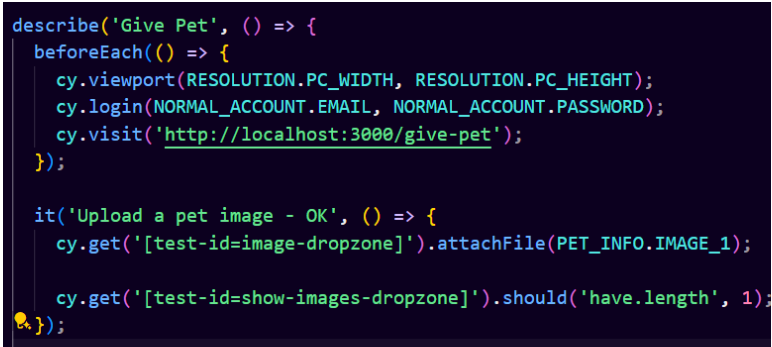
\includegraphics[width=0.7\textwidth]{Figures/cypress_script.png}
    \caption{Automation Script}
    \label{fig:cypress-script}
\end{figure}

\begin{figure}[H]
    \centering
    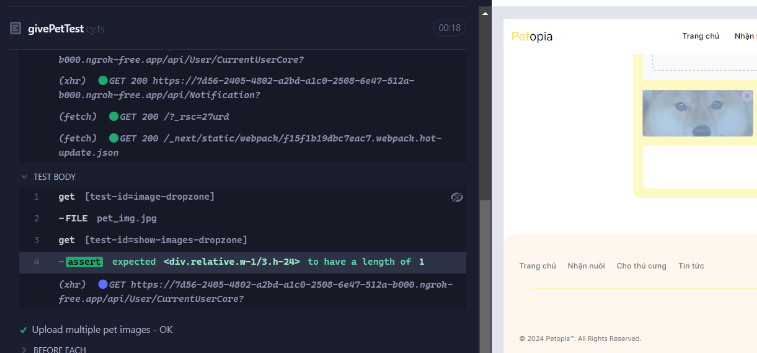
\includegraphics[width=0.7\textwidth]{Figures/cypress_auto.png}
    \caption{Automation tests done by Cypress}
    \label{fig:cypress-test}
\end{figure}

\subsection{Test Cases}
With Cypress, we tested our system features to make sure the system ran as expected and satisfied requirements. Below are some test-cases of the key features and test data for them, these test-cases were tested on multiple browser and environments.

\subsubsection*{Test data}

Normal User account:

\quad Email: vejox62251@facais.com - Password: 123456789

Organization User account:

\quad Email:  jayoki3306@facais.com - Password: 123456789

Owned-pet-id: baf3745f-d0d7-40c7-8084-5b55cb2f2ce3

\subsubsection*{Authentication}

\begin{longtblr}[
    caption = {Non-restricted Page Accessibility Test},
    label = {tblr:non_restricted_page_accessibility},
  ]{
    vline{1-3} = {-}{},
    hline{-} = {1-2}{},
    colspec={X[2,l] X[5, l]},
  }
  \textbf{Description} & \textbf{Non-restricted page accessibility} \\
  \textbf{Purpose} & {
    Test whether the guest user can access the pages that do not require authentication.
  } \\
  \textbf{Precondition} & {

  } \\
  \textbf{Steps} & {
    1. Click the “Nhận nuôi” button on the Nav bar.
    \\2. System shows the page content.
    \\3. Click the first pet card on the pet list.
    \\4. System shows the page content.
    \\5. Click the “Tin tức” button on the Nav bar.
    \\6. System shows the page content.
    \\7. Click the first blog card on the blog list.
    \\8. System shows the page content.
  } \\
  \textbf{Expected result} & {
    System does not direct the user to the login page.
  } \\
  \textbf{Execution results} & {
    PASSED
  } \\
\end{longtblr}




\begin{longtblr}[
    caption = {Restricted Page Accessibility Test},
    label = {tblr:restricted_page_accessibility},
  ]{
    vline{1-3} = {-}{},
    hline{-} = {1-2}{},
    colspec={X[2,l] X[5,l]},
  }
  \textbf{Description} & \textbf{Restricted page accessibility} \\
  \textbf{Purpose} & {
    Test whether the guest user can access the pages that do require authentication.
  } \\
  \textbf{Pre-condition} & {

  } \\
  \textbf{Steps} & {
    1. Click the “Cho thú cưng” button on the Nav bar.
  } \\
  \textbf{Expected result} & {
    System directs the user to the login page.
  } \\
  \textbf{Execution results} & {
    PASSED
  } \\
\end{longtblr}


\begin{longtblr}[
    caption = {Normal Account Accessibility Test},
    label = {tblr:normal_account_accessibility},
  ]{
    vline{1-3} = {-}{},
    hline{-} = {1-2}{},
    colspec={X[2,l] X[5,l]},
  }
  \textbf{Description} & \textbf{Normal account accessibility} \\
  \textbf{Purpose} & {
    Test whether the authenticated user with a normal account can access the pages that require authentication at the normal account level.
  } \\
  \textbf{Precondition} & {
    User logged in using a normal account.
  } \\
  \textbf{Steps} & {
    1. Click the “Cho thú cưng” button on the Nav bar.
  } \\
  \textbf{Expected result} & {
    System shows the restricted page content to the authenticated user.
  } \\
  \textbf{Execution results} & {
    PASSED
  } \\
\end{longtblr}


\begin{longtblr}[
    caption = {Organization Account Accessibility Test},
    label = {tblr:organization_account_accessibility},
  ]{
    vline{1-3} = {-}{},
    hline{-} = {1-2}{},
    colspec={X[2,l] X[5,l]},
  }
  \textbf{Description} & \textbf{Organization account accessibility} \\
  \textbf{Purpose} & {
    Test whether the authenticated user with an organization account can access the pages that require authentication at the organization account level.
  } \\
  \textbf{Precondition} & {
    User logged in using an organization account.
  } \\
  \textbf{Steps} & {
    1. Click the User avatar at top right.
    \\2. Click the User profile option.
    \\3. System directs to User profile page.
  } \\
  \textbf{Expected result} & {
    System shows the profile of the organization with the create blog option.
  } \\
  \textbf{Execution results} & {
    PASSED
  } \\
\end{longtblr}



\subsubsection*{Filter pet}

\begin{longtblr}[
    caption = {Filter Pets by Species Test},
    label = {tblr:filter_pets_by_species},
  ]{
    vline{1-3} = {-}{},
    hline{-} = {1-2}{},
    colspec={X[2,l] X[5,l]},
  }
  \textbf{Description} & \textbf{Filter pets by species} \\
  \textbf{Purpose} & {
    Test whether the pet list will be filtered by species.
  } \\
  \textbf{Precondition} & {
    User at search pet page.
  } \\
  \textbf{Steps} & {
    1. Click “Loài” button at the filter bar.
    \\2. Click option “Chó”.
  } \\
  \textbf{Expected result} & {
    System shows the list of dogs.
  } \\
  \textbf{Execution results} & {
    PASSED
  } \\
\end{longtblr}


The same test was done with other options: breed, age, color, sex, size, vaccinated, and spayed; which also yielded the same results. But there is a special case where breeds should be displayed according to the chosen species, so it is a separate case.

\begin{longtblr}[
    caption = {Breed Options Display According to Species Test},
    label = {tblr:breed_options_display},
  ]{
    vline{1-3} = {-}{},
    hline{-} = {1-2}{},
    colspec={X[2,l] X[5,l]},
  }
  \textbf{Description} & \textbf{Breed options display according to species} \\
  \textbf{Purpose} & {
    Test whether the breed options are displayed according to the chosen species.
  } \\
  \textbf{Precondition} & {
    User at search pet page.
  } \\
  \textbf{Steps} & {
    1. Click “Loài” button at the filter bar.
    \\2. Click option “Chó”.
    \\3. Click “Giống” button at the filter bar.
  } \\
  \textbf{Expected result} & {
    System shows a list of breeds of dogs available on the website.
  } \\
  \textbf{Execution results} & {
    PASSED
  } \\
\end{longtblr}


\subsubsection*{Account Configuration}

\begin{longtblr}[
    caption = {Update User Information Test},
    label = {tblr:update_user_information},
  ]{
    vline{1-3} = {-}{},
    hline{-} = {1-2}{},
    colspec={X[2,l] X[5,l]},
  }
  \textbf{Description} & \textbf{Update user information} \\
  \textbf{Purpose} & {
    Test whether the user can update information successfully.
  } \\
  \textbf{Precondition} & {
    User at the user profile page.
  } \\
  \textbf{Steps} & {
    1. Click the “Cập nhật thông tin” button.
    \\2. System shows the update information form.
    \\3. Fill in all the fields: First Name, Last Name, Email, Phone Number, Address.
    \\4. Click the submit button.
  } \\
  \textbf{Expected result} & {
    Account information is changed and displayed on the user profile page.
  } \\
  \textbf{Execution results} & {
    PASSED
  } \\
\end{longtblr}


\begin{longtblr}[
    caption = {Update User Information with Missing Last Name Test},
    label = {tblr:update_user_information_missing_last_name},
  ]{
    vline{1-3} = {-}{},
    hline{-} = {1-2}{},
    colspec={X[2,l] X[5,l]},
  }
  \textbf{Description} & \textbf{Update user information with missing field Last Name} \\
  \textbf{Purpose} & {
    Test whether the user can update information with a missing field.
  } \\
  \textbf{Precondition} & {
    User at the user profile page.
  } \\
  \textbf{Steps} & {
    1. Click the “Cập nhật thông tin” button.
    \\2. System shows the update information form.
    \\3. Fill in the fields: Last Name, Email, Phone Number, Address. Leave the field First Name empty.
    \\4. Click the submit button.
  } \\
  \textbf{Expected result} & {
    Submit form failed, system alerted user.
  } \\
  \textbf{Execution results} & {
    PASSED
  } \\
\end{longtblr}


The same test was done with other fields: last name, email, phone number, address; which also yielded the same results.

\subsubsection*{Give away pet}

\begin{longtblr}[
    caption = {Give Away Pet Test},
    label = {tblr:give_away_pet},
  ]{
    vline{1-3} = {-}{},
    hline{-} = {1-2}{},
    colspec={X[2,l] X[5,l]},
  }
  \textbf{Description} & \textbf{Give away pet} \\
  \textbf{Purpose} & {
    Test whether the user can give away a pet successfully.
  } \\
  \textbf{Precondition} & {
    User at the give pet page.
    \\ User is authenticated.
  } \\
  \textbf{Steps} & {
    1. System shows the give pet form. The first page is the pet image upload.
    \\2. Click the image upload zone. The system shows the upload window.
    \\3. Choose a .jpg image and click OK. The system shows the uploaded picture in the preview row.
    \\4. Click the “Tiếp tục” button. The system shows the pet information page.
    \\5. Fill in the pet information fields.
    \\6. Click the “Tiếp tục” button. The system shows pet giveaway terms.
    \\7. Tick the accept checkbox.
    \\8. Click the submit form button.
  } \\
  \textbf{Expected result} & {
    Submit pet giveaway form successfully.
  } \\
  \textbf{Execution results} & {
    PASSED
  } \\
\end{longtblr}


\begin{longtblr}[
    caption = {Submit Give Away Pet Form Without Uploading Pet Picture Test},
    label = {tblr:submit_give_away_pet_without_picture},
  ]{
    vline{1-3} = {-}{},
    hline{-} = {1-2}{},
    colspec={X[2,l] X[5,l]},
  }
  \textbf{Description} & \textbf{Submit give away pet form without uploading pet picture} \\
  \textbf{Purpose} & {
    Test whether the user can submit the give away pet form without uploading a picture of the pet.
  } \\
  \textbf{Precondition} & {
    User at the give pet page.
    \\ User is authenticated.
  } \\
  \textbf{Steps} & {
    1. System shows the give pet form. The first page is the pet image upload.
    \\2. Click the “Tiếp tục” button. System shows the pet information page.
    \\3. Fill in the pet information fields.
    \\4. Click the “Tiếp tục” button. System shows pet giveaway terms.
    \\5. Tick the accept checkbox.
    \\6. Click the submit form button.
  } \\
  \textbf{Expected result} & {
    Submit pet giveaway form fails. System alerts the user.
  } \\
  \textbf{Execution results} & {
    PASSED
  } \\
\end{longtblr}


\begin{longtblr}[
    caption = {Submit Give Away Pet Form Without Pet Information Test},
    label = {tblr:submit_give_away_pet_without_info},
  ]{
    vline{1-3} = {-}{},
    hline{-} = {1-2}{},
    colspec={X[2,l] X[5,l]},
  }
  \textbf{Description} & \textbf{Submit give away pet form without pet information} \\
  \textbf{Purpose} & {
    Test whether the user can submit the give away pet form without giving the information of the pet.
  } \\
  \textbf{Precondition} & {
    User at the give pet page.
    \\ User is authenticated.
  } \\
  \textbf{Steps} & {
    1. System shows the give pet form. The first page is the pet image upload.
    \\2. Click the image upload zone. System shows the upload window.
    \\3. Choose a .jpg image and click OK. The system shows the uploaded picture in the preview row.
    \\4. Click the “Tiếp tục” button. System shows the pet information page.
    \\5. Click the “Tiếp tục” button. System shows pet giveaway terms.
    \\6. Tick the accept checkbox.
    \\7. Click the submit form button.
  } \\
  \textbf{Expected result} & {
    Submit pet giveaway form fails. System alerts the user.
  } \\
  \textbf{Execution results} & {
    PASSED
  } \\
\end{longtblr}


\begin{longtblr}[
    caption = {Submit Give Away Pet Form Without Reading Give Away Terms Test},
    label = {tblr:submit_give_away_pet_without_terms},
  ]{
    vline{1-3} = {-}{},
    hline{-} = {1-2}{},
    colspec={X[2,l] X[5,l]},
  }
  \textbf{Description} & \textbf{Submit give away pet form without reading give away terms} \\
  \textbf{Purpose} & {
    Test whether the user can submit the give away pet form without reading the terms.
  } \\
  \textbf{Precondition} & {
    User at the give pet page.
    \\ User is authenticated.
  } \\
  \textbf{Steps} & {
    1. System shows the give pet form. The first page is the pet image upload.
    \\2. Click the “Tiếp tục” button. System shows the pet information page.
    \\3. Click the “Tiếp tục” button. System shows pet giveaway terms.
    \\4. Try to tick the accept checkbox.
  } \\
  \textbf{Expected result} & {
    Cannot tick the accept checkbox. System alerts the user.
  } \\
  \textbf{Execution results} & {
    PASSED
  } \\
\end{longtblr}


\subsubsection*{Adopt Pet}

\begin{longtblr}[
    caption = {Adopt Pet Test},
    label = {tblr:adopt_pet},
  ]{
    vline{1-3} = {-}{},
    hline{-} = {1-2}{},
    colspec={X[2,l] X[5,l]},
  }
  \textbf{Description} & \textbf{Adopt pet} \\
  \textbf{Purpose} & {
    Test whether the user can submit an adopt application successfully.
  } \\
  \textbf{Precondition} & {
    User at the search pet page.
    \\ User is authenticated.
  } \\
  \textbf{Steps} & {
    1. Click the first pet card on the pet list.
    \\2. System directs to the pet detail page.
    \\3. Click the “Nhận nuôi” button.
    \\4. System shows the adopt application form.
    \\5. Fill in all required information: name, email, phone number, address, home type, adopt time, note, pets owned.
    \\6. Click the submit button.
  } \\
  \textbf{Expected result} & {
    User submits adopt application successfully.
  } \\
  \textbf{Execution results} & {
    PASSED
  } \\
\end{longtblr}


\begin{longtblr}[
    caption = {Submit Adopt Pet on Already Submitted Pet Test},
    label = {tblr:submit_adopt_pet_again},
  ]{
    vline{1-3} = {-}{},
    hline{-} = {1-2}{},
    colspec={X[2,l] X[5,l]},
  }
  \textbf{Description} & \textbf{Submit adopt pet on already submitted pet} \\
  \textbf{Purpose} & {
    Test whether the user can submit an adopt application again on the same pet.
  } \\
  \textbf{Precondition} & {
    User at the search pet page.
    \\ User is authenticated.
    \\ Already done the Adopt pet test case.
  } \\
  \textbf{Steps} & {
    1. Click the first pet card on the pet list.
    \\2. System directs to the pet detail page.
    \\3. Click the “Nhận nuôi” button.
  } \\
  \textbf{Expected result} & {
    System alerts the user that they already sent the adopt application for this pet.
  } \\
  \textbf{Execution results} & {
    PASSED
  } \\
\end{longtblr}


\begin{longtblr}[
    caption = {Adopt Owned Pet Test},
    label = {tblr:adopt_owned_pet},
  ]{
    vline{1-3} = {-}{},
    hline{-} = {1-2}{},
    colspec={X[2,l] X[5,l]},
  }
  \textbf{Description} & \textbf{Adopt owned pet} \\
  \textbf{Purpose} & {
    Test whether the user can submit an adopt application for a pet that has already been adopted.
  } \\
  \textbf{Precondition} & {
    User is authenticated.
    \\ System has owned pet.
  } \\
  \textbf{Steps} & {
    1. Use the owned pet ID in the test data to visit the pet detail page by adding “/pet/[pet-id]” to the website URL.
    \\2. System directs to the pet detail page.
  } \\
  \textbf{Expected result} & {
    The “Nhận nuôi” button is not available.
  } \\
  \textbf{Execution results} & {
    PASSED
  } \\
\end{longtblr}


\subsubsection*{Blog}

\begin{longtblr}[
    caption = {Blog Browsing - Blog Card Linking Test},
    label = {tblr:blog_card_linking},
  ]{
    vline{1-3} = {-}{},
    hline{-} = {1-2}{},
    colspec={X[2,l] X[5,l]},
  }
  \textbf{Description} & \textbf{Blog browsing - Blog card linking} \\
  \textbf{Purpose} & {
    Test whether the blog card directs to the correct blog.
  } \\
  \textbf{Precondition} & {
    User at the blog page.
  } \\
  \textbf{Steps} & {
    1. Click the first blog card.
    \\2. System directs to the blog detail page.
  } \\
  \textbf{Expected result} & {
    System displays the blog detail page related to the chosen blog card.
  } \\
  \textbf{Execution results} & {
    PASSED
  } \\
\end{longtblr}


\begin{longtblr}[
    caption = {Blog Browsing - Filter Blog by Health Category Test},
    label = {tblr:filter_blog_by_health_category},
  ]{
    vline{1-3} = {-}{},
    hline{-} = {1-2}{},
    colspec={X[2,l] X[5,l]},
  }
  \textbf{Description} & \textbf{Blog browsing - Filter blog by health category} \\
  \textbf{Purpose} & {
    Test whether the blog cards will be filtered by the category bar.
  } \\
  \textbf{Precondition} & {
    User at the blog page.
  } \\
  \textbf{Steps} & {
    1. Click the “Sức khỏe” option in the category bar.
    \\2. System displays new filtered blog cards.
  } \\
  \textbf{Expected result} & {
    System only displays the blogs about health.
  } \\
  \textbf{Execution results} & {
    PASSED
  } \\
\end{longtblr}


The same test was done with other categories: art, training, and product; which also yielded the same results.

\begin{longtblr}[
    caption = {Blog Create Test},
    label = {tblr:blog_create},
  ]{
    vline{1-3} = {-}{},
    hline{-} = {1-2}{},
    colspec={X[2,l] X[5,l]},
  }
  \textbf{Description} & \textbf{Blog create} \\
  \textbf{Purpose} & {
    Test whether the user can create a blog.
  } \\
  \textbf{Precondition} & {
    User is logged in using an organization account.
    \\ User is at the user profile page.
  } \\
  \textbf{Steps} & {
    1. Click the blog tab. System displays the blog tab content.
    \\2. Click the create blog card.
    \\3. System directs to the blog create page.
    \\4. Fill in the required fields: title, excerpt, blog image, blog content.
    \\5. Click the submit button.
  } \\
  \textbf{Expected result} & {
    User creates the blog successfully.
  } \\
  \textbf{Execution results} & {
    PASSED
  } \\
\end{longtblr}


\begin{longtblr}[
    caption = {Blog Update Test},
    label = {tblr:blog_update},
  ]{
    vline{1-3} = {-}{},
    hline{-} = {1-2}{},
    colspec={X[2,l] X[5,l]},
  }
  \textbf{Description} & \textbf{Blog Update} \\
  \textbf{Purpose} & {
    Test whether the user can update a created blog.
  } \\
  \textbf{Precondition} & {
    User is logged in using an organization account.
    \\ User is at the user profile page.
    \\ Have done the previous Blog Create Test-case.
  } \\
  \textbf{Steps} & {
    1. Click the blog tab. System displays the blog tab content.
    \\2. Click the edit button on the created blog.
    \\3. System opens the blog update form.
    \\4. Change the blog title, content, excerpt, image.
    \\5. Click the submit button.
  } \\
  \textbf{Expected result} & {
    User updates the blog successfully.
  } \\
  \textbf{Execution results} & {
    PASSED
  } \\
\end{longtblr}


\section{Responsive testing}
Responsive testing is a crucial aspect of web development, ensuring that
websites are accessible and user-friendly across different devices and
screen sizes. By testing the website's responsiveness, we could verify
that it displayed correctly on various devices, including desktops,
laptops, tablets, and smartphones. This testing process involved
evaluating the website's layout, design, and functionality on different
devices, ensuring a consistent and seamless user experience. By
identifying and addressing any responsiveness issues, we could enhance
the website's usability and accessibility, catering to a broader audience
and improving user satisfaction.

Here is the checklist for responsive testing:
\begin{longtblr}[
    caption = {Responsive Testing Checklist},
    label = {tblr:responsive_testing},
  ]{
    hlines, vlines,
    colspec = {X[2,l] X[4,l] X[4,l]},
    row{1} = {font=\bfseries},
  }
  Category                                & Checklist Item                                       & Notes                                        \\
  \SetCell[r=3]{t}Devices                 & Test on mobile phones                                & Common devices: iPhone, Android, etc.        \\
                                          & Test on tablets                                      & Common devices: iPad, Android tablets, etc.  \\
                                          & Test on laptops and desktops                         & Different screen resolutions                 \\
  \SetCell[r=4]{c}Screen Sizes            & Test on small screens (e.g., 320px width)            & Minimum screen width                         \\
                                          & Test on medium screens (e.g., 768px width)           & Common tablet screen width                   \\
                                          & Test on large screens (e.g., 1024px width and above) & Common laptop/desktop screen widths          \\
                                          & Test on extra-large screens (e.g., 1920px width)     & Large desktop/monitor screen widths          \\
  \SetCell[r=2]{c}Orientation             & Test in portrait mode                                & Vertical screen orientation                  \\
                                          & Test in landscape mode                               & Horizontal screen orientation                \\
  \SetCell[r=5]{c}Browsers                & Test on Chrome                                       & Most widely used browser                     \\
                                          & Test on Firefox                                      & Popular alternative browser                  \\
                                          & Test on Safari                                       & Default browser on iOS devices               \\
                                          & Test on Edge                                         & Default browser on Windows devices           \\
                                          & Test on Opera                                        & Another popular browser option               \\
  \SetCell[r=2]{c}Performance             & Check page load speed                                & Tools: Google PageSpeed Insights, GTmetrix   \\
                                          & Check image optimization                             & Ensure images are responsive and compressed  \\
                                          & Test navigation menus                                & Ensure menus work and are accessible         \\
  \SetCell[r=4]{c}Functionality           & Test forms (input fields, buttons, etc.)             & Ensure all forms are functional              \\
                                          & Test buttons and links                               & Ensure they are easily clickable             \\
                                          & Test media (videos, sliders, etc.)                   & Ensure media is responsive and playable      \\
                                          & Test interactive elements (e.g., accordions, modals) & Ensure they work as expected                 \\
  \SetCell[r=3]{c}Content                 & Check text readability                               & Ensure text is readable at all sizes         \\
                                          & Check image and video scaling                        & Ensure media scales properly                 \\
                                          & Check layout consistency                             & Ensure layout remains consistent             \\
  \SetCell[r=3]{c}Accessibility           & Test keyboard navigation                             & Ensure site can be navigated with a keyboard \\
                                          & Check for screen reader compatibility                & Ensure compatibility with screen readers     \\
                                          & Check color contrast and text size                   & Ensure sufficient contrast and readability   \\
  \SetCell[r=5]{c, valign=t}Miscellaneous & Test touch gestures                                  & Ensure touch gestures work (e.g., swiping)   \\
                                          & Check for any horizontal scrolling                   & Avoid horizontal scrolling                   \\
                                          & Test for viewport meta tag                           & Ensure correct viewport settings             \\
                                          & Check for broken links                               & Ensure no broken links                       \\
                                          & Test social media sharing buttons                    & Ensure they work and are properly positioned \\
\end{longtblr}


\section{Performance testing}
For performance testing, we use Google Lighthouse to help us evaluate general performance, accessibility, best practice and SEO parameters of our website:
\begin{itemize}
  \item Performance: Measures how quickly a page loads and becomes interactive.
  \item Accessibility: Assesses how well a page can be used by people with disabilities.
  \item Best Practices: Checks adherence to best practices for web development.
  \item SEO: Evaluates how well a page is optimized for search engines.
\end{itemize}
Google Lighthouse uses a 0 to 100 scale to evaluate web page performance and other metrics. Here’s a breakdown:
\begin{itemize}
  \item 90 - 100: Excellent performance.
  \item 50 - 89: Average performance.
  \item 0 - 49: Poor performance.
\end{itemize}

\begin{table}[H]
  \caption{Performance testing result}
  \label{Performance testing result}
  \centering
  {
    \renewcommand{\arraystretch}{1.5}
      \begin{tabular}{|c|c|c|c|c|}
      \hline
                          & \textbf{Performance}       & \textbf{Accessibility}     & \textbf{Best practices}    & \textbf{SEO}                                       \\ \hline
      Home page          & \cellcolor[HTML]{32CB00}96 & \cellcolor[HTML]{FFFC9E}83 & \cellcolor[HTML]{FFFC9E}78 & \cellcolor[HTML]{32CB00}90                         \\ \hline
      Search page        & \cellcolor[HTML]{FFFC9E}74 & \cellcolor[HTML]{FFFC9E}83 & \cellcolor[HTML]{FFFC9E}78 & \cellcolor[HTML]{32CB00}90                         \\ \hline
      Pet detail page    & \cellcolor[HTML]{FFFC9E}87 & \cellcolor[HTML]{FFFC9E}80 & \cellcolor[HTML]{FFFC9E}78 & \cellcolor[HTML]{FFFC9E}70                         \\ \hline
      Blogs page         & \cellcolor[HTML]{FFFC9E}82 & \cellcolor[HTML]{FFFC9E}85 & \cellcolor[HTML]{FFFC9E}78 & \cellcolor[HTML]{32CB00}90                         \\ \hline
      Blog detail page   & \cellcolor[HTML]{FFFC9E}87 & \cellcolor[HTML]{FFFC9E}80 & \cellcolor[HTML]{FFFC9E}78 & \cellcolor[HTML]{FFFC9E}70                         \\ \hline
      User profile page  & \cellcolor[HTML]{FFFC9E}71 & \cellcolor[HTML]{FFFC9E}82 & \cellcolor[HTML]{FFFC9E}78 & \cellcolor[HTML]{32CB00}90                         \\ \hline
      Give-pet page      & \cellcolor[HTML]{FFFC9E}79 & \cellcolor[HTML]{FFFC9E}85 & \cellcolor[HTML]{FFFC9E}78 & \cellcolor[HTML]{32CB00}90                         \\ \hline
      Register page      & \cellcolor[HTML]{32CB00}98 & \cellcolor[HTML]{32CB00}95 & \cellcolor[HTML]{FFFC9E}78 & \cellcolor[HTML]{32CB00}100                        \\ \hline
      Login page         & \cellcolor[HTML]{FFFC9E}84 & \cellcolor[HTML]{32CB00}95 & \cellcolor[HTML]{FFFC9E}78 & \cellcolor[HTML]{32CB00}100                        \\ \hline
      Advertisement page & \cellcolor[HTML]{FFFC9E}78 & \cellcolor[HTML]{FFFC9E}82 & \cellcolor[HTML]{FFFC9E}78 & \cellcolor[HTML]{FFFC9E}70                         \\ \hline
      \end{tabular}
  }
  \end{table}

From \textit{Table 6.31}, It can be said that the website passed the performance test with all measured parameters being greater than 50, especially SEO with most of the measured values being greater than 90.

\section{Load testing}
API load testing involves simulating real-world traffic and observing API’s resulting behavior. It is conducted to evaluate how well an API meets performance expectations for response time, throughput, and availability under the simulated load.

For this type of testing, we use Postman with the pre-conditions:
\begin{itemize}
  \item Set of APIs: \textit{ Create a pet -> Get pets -> Update a pet -> Get pets again}
  \item Duration: \textit{30 seconds}
  \item Number of vitual users: \textit{50}
  \item Ramp up: \textit{from 5 users at the begining to 50 users at the end of the duration}
\end{itemize}

Base on the non-functional requirements of the system, the expected outputs are:
\begin{itemize}
  \item Error rate: \textit{less than 5\% for at least 1000 requests}
  \item Average response time: \textit{less than 1000ms for 1000 requests}
\end{itemize}

After doing the test, the final result is shown in \textit{Figure 6.3}. All the expected outputs are passed with the the outputs are:
\begin{itemize}
  \item Error rate: \textit{0\% for 1704 requests}
  \item Average response time: \textit{17ms for 1704 requests}
\end{itemize}

\begin{figure}[H]
  \centering
  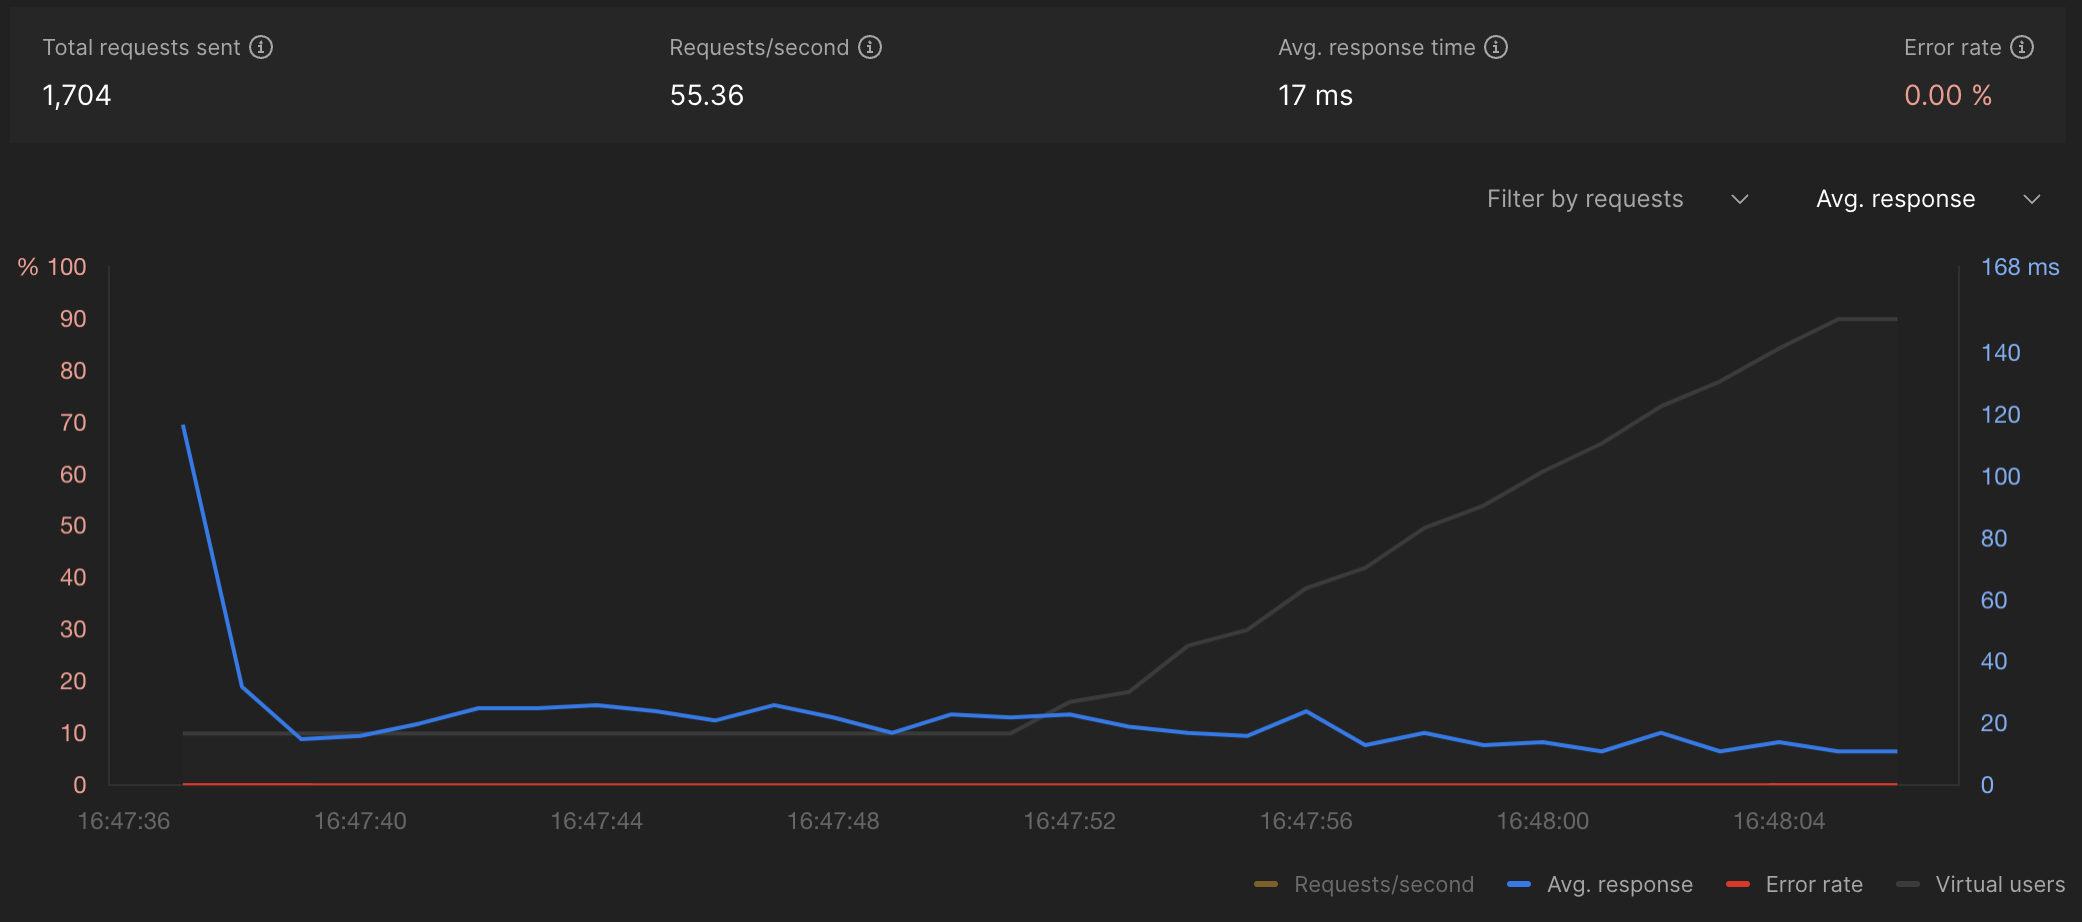
\includegraphics[width=0.9\textwidth]{Figures/load_test.png}
  \caption{Load test outputs}
\end{figure}

\chapter{DEPLOYMENT PLAN} 
With the completion of system testing and evaluation, we are now 
focusing on serving the system to the end users. This section will 
discuss the detailed deployment architecture and services. As we 
can see from Figure X, the proposed architecture contains the 
following components:
\begin{figure}[H]
    \centering
    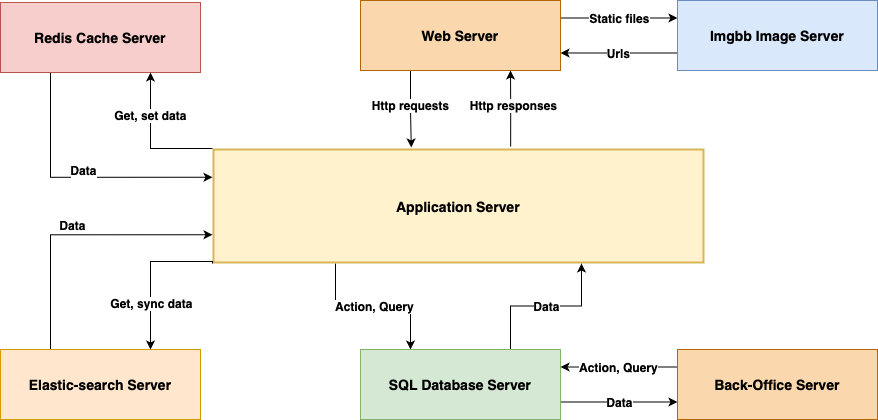
\includegraphics[width=0.7\textwidth]{Figures/Deployment/Pattern and Architecture-Deployment.drawio.png}
    \caption{Automation Script}
    \label{fig:cypress-script}
\end{figure}
The Web Server contains the Presentation layer of the system. It is the place that receives requests and sends 
back the web application or website to user browsers. It also 
handles user events and calls restful API from the Application 
Servers. A free Vercel cloud pipeline is used for this component.

The Application Servers contain the Business and Data Access layers 
of the system. This is the central part of the system, focusing on 
handling all business logic and flow, serving API for the web server, 
and interacting with other components of the system. We will use an Azure 
Virtual Machine to serve this component.

SQL Database Server is the place where the database of the system is served. 
This server interacts with the Application Server and Back-Office Server. 
This component will be deployed using an Azure SQL Database.

Imgbb Image Server stores all the static images of the system. Images will 
be uploaded directly from the Web Server to the Imgbb Image Server before 
storing the returned URLs in the SQL Database Server. This component will 
be served by a free Imgbb cloud service.

Finally, we will have two corresponding servers for caching data and optimizing 
data search speed using a free Elastic-search cloud and Azure Redis Cache Database.

\chapter*{Conclusion}


\input{manually.bbl}

\end{document}
